\documentclass[11pt,a4paper]{article}
\usepackage[utf8]{inputenc}
\usepackage[T1]{fontenc}
\usepackage[english]{babel}
\usepackage{amsmath,amssymb}
\usepackage{geometry}
\usepackage{hyperref}
\usepackage{xcolor}
\usepackage{booktabs}
\usepackage[most]{tcolorbox}
\usepackage{colortbl}

\geometry{margin=2.5cm}

\title{\Large \textbf{Research Internship Report}\\ \huge \textbf{Self-Improvement of LLM Agents in Multi-Turn Environments}\\ \large Criteo AI Lab}
\author{\textbf{Vadim Lagresle} \\ Supervisors: Alberto Lumbreras, Patrick Gallinari, Alain Rakotomamonjy, Sylvain Lamprier}
\date{\today}

\begin{document}

\maketitle

\vspace{2cm}



\begin{abstract}
\noindent This report presents an experimental study of the reinforcement learning post-training of agents built on language models, in interactive multi-turn environments. Scaling up training environments, through their diversity, their difficulty and their verifiers, has become the main driver of agentic capabilities. Our question is the one that arises once the environment is given: how to stabilize learning in it, and how to make it efficient. We study it on TextCraft, an environment from the AgentGym-RL ecosystem with a verifiable reward, with a view to adapting these methods to Criteo's shopping agents.

Our two main contributions address these two questions of efficiency and stabilization. Efficiency comes from LoRA, a low-rank adaptation that trains only a small fraction of the model's weights and makes experimentation possible on a single GPU; we show under which conditions it remains stable in the multi-turn setting. Stability comes from curricula, that is, training regimes that progressively increase the difficulty of the episodes presented to the agent, through the number of turns, the generation budget or the complexity of the tasks. With an identical recipe and controlled compute, training without a curriculum collapses where all three curricula hold. The best one brings a three-billion-parameter model to 82\,\% success, above the result published by the reference system on a multi-GPU infrastructure, and the whole training run is documented so that it can be reproduced.

This path thus provides a detailed account of the obstacles encountered, from observation masking to reward design, which may save time in the development of Criteo's shopping agents. Finally, we analyze these results beyond stabilization: what the curriculum changes in the order in which difficulties are acquired and in the elimination of errors, what it says about the hypothesis that reinforcement merely concentrates the capabilities of the base model, and how it opens onto broader questions of meta-learning and continual learning.
\end{abstract}



\newpage




\section*{Acknowledgements}
\addcontentsline{toc}{section}{Acknowledgements}

I would first like to thank Patrick Gallinari, Alberto Lumbreras and Alain Rakotomamonjy, who have followed my work every week since the beginning of this internship and whose advice has meant a great deal. My thanks also go to Maxime, my manager, and to the Agentic Commerce team and the Agentic Core Team at Criteo, for introducing me to their missions, their expertise and the agentic context of the company. Finally, I am grateful to Sylvain Lamprier for his reading suggestions on autotelic agents and the hierarchical organization of skills, to Flavian and Imad for introducing me to DeepShopper, an internal Criteo project, and to Otmane Sakhi for our discussions on self-normalized importance sampling.








\vspace{0.5cm}

\newpage
\setcounter{tocdepth}{2} % Limits the table of contents to sections and subsections (excludes subsubsections)
\tableofcontents

\newpage
\section*{Notations and Abbreviations}
\addcontentsline{toc}{section}{Notations and Abbreviations}

\subsection*{Notations}
\begin{tabular}{ll}
\toprule
Symbol & Meaning \\
\midrule
$\pi_\theta$ & trained policy, parameterized by the weights $\theta$ \\
$\pi_{\text{ref}}$ & reference policy of the KL penalty (anchor) \\
$\tau$ & trajectory (complete episode) \\
$s_t,\ a_t,\ o_t$ & state, action and observation at step $t$ \\
$T$ & episode horizon (maximum number of turns) \\
$R(\tau)$, $R_i$ & terminal reward of a trajectory; that of rollout $i$ \\
$\hat{A}$, $\hat{A}_i$ & advantage estimator; relative advantage of rollout $i$ within its group \\
$V_\phi$ & value function estimated by the critic network (PPO) \\
$r_t(\theta)$ & importance ratio $\pi_\theta(a_t \mid s_t)/\pi_{\theta_{\text{old}}}(a_t \mid s_t)$ \\
$G$ & GRPO group size (trajectories per task within a single group) \\
$k$ & number of independent samples per task (pass@$k$ budget) \\
$\beta$ & coefficient of the penalty $D_{\text{KL}}(\pi_\theta \parallel \pi_{\text{ref}})$ \\
$\epsilon$ & \emph{clipping} radius of the PPO/GRPO objective \\
$r,\ \alpha$ & rank and scaling factor of a LoRA adapter \\
$d$ & depth of a TextCraft task, $d \in \{1,\dots,4\}$ \\


\bottomrule
\end{tabular}

\medskip
\noindent\textbf{pass@$k$.} Fraction of the tasks in the evaluation set solved by
at least one of $k$ independent draws from the policy. The pass@$1$
measures the reliability of a single draw; the pass@$k$ for large $k$ approaches the
support of the policy. Every pass@$k$ value is reported together with its budget
$k$ and its sampling temperature.

\subsection*{Abbreviations}
\begin{tabular}{ll}
\toprule
Abbreviation & Meaning \\
\midrule
LLM & \emph{Large Language Model} \\
SFT & \emph{Supervised Fine-Tuning} \\
RL & reinforcement learning \\
RLHF & RL from human feedback \\
RLVR & RL with verifiable rewards \\
NLL & negative log-likelihood \\
TRPO & \emph{Trust Region Policy Optimization} \\
PPO & \emph{Proximal Policy Optimization} \\
GRPO & \emph{Group Relative Policy Optimization} \\
DPO & \emph{Direct Preference Optimization} \\
KL & Kullback-Leibler divergence \\
(PO)MDP & (partially observable) Markov decision process \\
LoRA & \emph{Low-Rank Adaptation} \\
CoT & \emph{Chain-of-Thought} \\
PRM & \emph{Process Reward Model} \\
MCP & \emph{Model Context Protocol} \\
SNIS & self-normalized importance sampling \\
\bottomrule
\end{tabular}



\newpage




\section{Introduction}

\subsection{Evolution of the Learning Signal}

\emph{Self-improving agents} are today among the most active topics in machine learning. This is visible in the university courses devoted to them, such as Stanford's recent CS329A~\cite{cs329a}, in the number of publications at the field's major conferences, and in the investments of model developers. To understand why this topic attracts so much attention, it is useful to trace the evolution of the learning signal of LLMs over the past decade. Beyond the opportunities opened up by agentic applications, this evolution extends the field's previous shifts: each time, it is the nature of the data, and of the signal extracted from it, that has changed.

The initial breakthrough introduced by the Transformer architecture \cite{vaswani2017attention} made it possible to scale up the autoregressive autocompletion task, predicting the next token on immense text corpora drawn from the web. This massive pre-training endows the model with a broad linguistic representation of the world. However, this learning signal remains implicit and passive: the model learns to imitate the distribution of web text with no guarantee of alignment with the requirements of accuracy, logic, or safety expected by a human user.

To overcome these limitations, the post-training phase has established itself as the central stage of behavioral alignment. First, \emph{Supervised Fine-Tuning} structured the form of responses to instructions~\cite{wei2022flan}. Subsequently, reinforcement learning from human preferences (RLHF) \cite{ouyang2022training} introduced a global evaluation signal, making it possible to penalize toxic or off-topic responses. More recently, efforts have focused on the emergence of complex reasoning capabilities, where the model is encouraged to produce a reasoning trace (\emph{Chain-of-Thought}) before its answer \cite{wei2022cot}. In this setting, the nature of the signal has once again evolved toward deterministically verifiable rewards ($0$ or $1$), notably in mathematics or programming, which make it possible to assess the correctness of a chain of thought without relying on subjective human annotations. This reinforcement learning with verifiable rewards (RLVR) has made it possible to scale LLMs on complex reasoning tasks, and it lies at the heart of the performance of current models \cite{openai_o1_2024, deepseekr1_2025}. Its practical appeal is twofold: it dispenses with both the training and the inference of a reward model, and it reconnects with the classical questions of reinforcement learning, framed in terms of objectives, tasks, and environments, which the LLM wave had temporarily eclipsed. Many applications remain out of reach of RLVR for now, such as summary evaluation or recommendation; we do not address them here, and aim to master the techniques that scale before tackling their specific applications.

Within the RLVR framework, training trajectories now run into a critical material and economic limit: the scarcity and high cost of high-quality human data in demanding domains. Annotated data has become the major bottleneck of the discipline, which forces a paradigm shift toward synthetic data generation and autonomous learning. Self-improvement approaches such as STaR \cite{zelikman2022star} or ReST \cite{singh2024beyond} have shown that a model can generate its own reasoning traces, filter the trajectories that lead to the correct answer, and then retrain on its own successes. This iterative process increases the model's autonomy while considerably reducing its dependence on direct human supervision.

An influential theoretical thesis interprets this dynamic with skepticism: self-improvement on synthetic data would create no fundamentally new information, and would amount to a \emph{sharpening} mechanism \cite{huang2024self}, in which retraining concentrates the policy's probability mass on high-reward trajectories, amortizing the cost of inference-time compute without extending capabilities. This report treats this thesis as a working hypothesis to be put to the test, not as an established fact: a substantial part of our study consists precisely in measuring whether an adequate structuring of learning makes it possible to go beyond the boundaries that this reading predicts. The emergence of agentic AI is a direct continuation of this evolution: it is no longer merely a matter of generating a reasoning trace in a single shot, but of deploying these capabilities within interactive digital environments, where the agent learns autonomously from the feedback of its actions.

Finally, the agentic setting recasts the data bottleneck in a new form: what must now scale is no longer a static corpus of texts or annotations, but the interaction environment itself, that is, the joint definition of an initial state, a tool surface, a task, and a verifier. Recent technical reports from model developers converge on this point. The Qwen team explicitly identifies the scaling of environments (\emph{environment scaling}) as the central obstacle of agentic RL \cite{qwen3coder2025}, and attributes most of the gains of its latest generations to the massive extension of the difficulty and diversity of its training tasks \cite{qwen35_2026}. Kimi K2 grounds its agentic capabilities in a large-scale pipeline synthesizing tools, tasks, and verified trajectories, coupled with joint RL training on real and simulated environments \cite{kimik2_2025}. Symmetrically, the field's reference benchmarks ($\tau^2$-bench \cite{tau2bench2025}, Toolathlon \cite{toolathlon2025}, MCP-Atlas \cite{mcpatlas2026}) are less datasets than problem-definition efforts: building a task there means specifying a world, its rules, and its success criterion. The definition of the environment thus becomes a scientific object in its own right, just as corpus curation was for pre-training. This observation structures the whole of this report.

\subsection{Background and Similarities of the Training Algorithms}

We assume that the reader is familiar with Transformer and natural language processing techniques, and refer to the Stanford courses on language modeling (\href{https://cs336.stanford.edu/}{CS336}) and on large language models (\href{https://stanford-cs324.github.io/winter2022/}{CS324}) for a complete presentation. Likewise, this subsection presents only the elements of reinforcement learning needed to read the report, in particular GRPO, our working algorithm. Appendix~A develops the full formalism, from the classical RL framework (POMDP) to actor-critic methods; for an in-depth treatment of deep RL, we refer to the Stanford (\href{https://cs224r.stanford.edu/}{CS224R}) and Berkeley (\href{https://rail.eecs.berkeley.edu/deeprlcourse/}{CS285}) courses.

The evolution of the nature of the data and of the learning signal has gone hand in hand with a diversity of optimization algorithms used at each phase. Pre-training relies on the Transformer architecture \cite{vaswani2017attention}, which supplanted recurrent and sequential architectures. The latter suffered from a computational bottleneck preventing parallelization and from a vanishing-gradient phenomenon over long contexts. The self-attention mechanism makes it possible to compute in parallel the dependencies between all tokens of a sequence, regardless of their relative distance. This capacity for massive parallelization on GPUs made it possible to process raw web corpora at very large scale.

In the same vein, the \emph{Supervised Fine-Tuning} phase keeps the same autoregressive architecture and the same token-prediction principle as pre-training, but differs from it by three technical adjustments, beyond the limited volume and high quality of the data. First, the injection of structuring control tokens (\emph{chat templates}) turns continuous text into a state machine alternating between user and assistant roles, which conditions generation toward conversational-agent behavior. Second, the optimization regime is adapted: a markedly lower learning rate over a reduced number of epochs concentrates the probability mass on the expected response structures, without destroying the acquired representations. Finally, whereas pre-training computes the gradient over the entire text, SFT applies \emph{loss masking} to the tokens of the instruction $x = (x_1, \dots, x_N)$, so as to backpropagate the signal only on the tokens of the target response $y = (y_1, \dots, y_M)$. The model minimizes the average negative log-likelihood computed exclusively over the $M$ tokens of the response:
\begin{equation}
\mathcal{L}_{\text{SFT}}(\theta) = -\frac{1}{M} \sum_{m=1}^{M} \log \pi_\theta(y_m \mid x, y_{<m})
\end{equation}

Unlike SFT, whose weight-update mechanics remain close to those of pre-training, reinforcement-based alignment introduces a fundamentally different signal and optimization framework. It is worth first establishing the fundamental difference between the two. In fine-tuning, the model learns to reproduce a target sequence token by token: the learning signal is the next token given the preceding sequence. In RL, the signal is the \emph{reward}, a scalar quantifying the overall quality of a response produced by the agent. The objective becomes to favor the trajectories leading to the highest rewards: in the case of a binary \emph{sparse} reward, typical of mathematical benchmarks for instance, the trajectories that reached the correct answer are reinforced and the others are penalized. One speaks of \emph{reinforcement} learning because the algorithm reinforces the model's output distribution toward a target distribution that it already contained, in embryonic form, at the end of pre-training.

To exploit a scalar reward signal $R(\tau)$ defined over an entire trajectory $\tau$, one must express a gradient, but the reward is rarely differentiable, unlike the loss functions used in supervised fine-tuning. Policy gradient methods rely on the REINFORCE trick (log-derivative), which rewrites the gradient of the expected reward in a form computable by Monte Carlo sampling:
\begin{equation}
\nabla_\theta \mathbb{E}_{\tau \sim \pi_\theta}[R(\tau)] = \mathbb{E}_{\tau \sim \pi_\theta} \left[ \sum_{t=1}^T \nabla_\theta \log \pi_\theta(a_t \mid s_t) R(\tau) \right]
\end{equation}
Without this rewriting, the gradient could not be estimated by sampling.

\textbf{Remark.} SFT and RL are not fundamentally far apart in their weight-update mechanics, although the underlying theories differ. Under a \emph{sparse} reward and a strictly \emph{on-policy} strategy, that is, when training is performed on generations produced by the current policy (Appendix~A), the policy gradient algorithm reduces exactly to an SFT applied only to the trajectories that reached the correct answer. This equivalence illustrates both the richness and the instability of RL: it identifies without human annotation the trajectories to favor, but the only available signal is final success, whereas erroneous strategies can occasionally lead to the correct answer. The low annotation cost is paid for by a greater difficulty in stabilization, as these algorithms can \emph{collapse} within a few iterations; Sections~2.3 and~4.2 return to this in detail.

Used alone, the reward $R(\tau)$ is a raw signal: it does not say whether a trajectory is good in itself, only what gain it yielded, with no point of comparison. The actor-critic framework introduces a critic network $V_\phi(s)$, trained to estimate the value function, that is, the expected return obtained from state $s_t$ when following the current policy. This quantity depends only on the state, not on the action taken: it provides a reference that recenters the signal in the form of an advantage, whose simplest estimator is $\hat{A}_t = R_t - V_\phi(s_t)$ (Appendix~A details the estimators used in practice). Substituting $\hat{A}_t$ for $R(\tau)$ amounts to reinforcing an action only insofar as it did better than the expected average, which considerably reduces variance. To this structure is added, for LLMs, a Kullback-Leibler divergence penalty anchoring the trained policy $\pi_\theta$ to a frozen reference policy $\pi_{\text{ref}}$, usually the model resulting from SFT, in order to avoid catastrophic drift and the forgetting of base capabilities:
\begin{equation}
\mathcal{L}_{\text{RL}}(\theta) = -\mathbb{E}_{(s_t, a_t)} \left[ \log \pi_\theta(a_t \mid s_t) \hat{A}_t \right] + \beta \, D_{\text{KL}}(\pi_\theta \parallel \pi_{\text{ref}})
\end{equation}

\emph{Proximal Policy Optimization} (PPO) \cite{schulman2017proximal} belongs to this actor-critic framework; designed for control and robotics well before modern LLMs, it was adopted from 2022 onward as the central algorithm of RLHF \cite{ouyang2022training}. Reusing the same batch of trajectories for several gradient steps considerably improves data efficiency, but requires correcting for the gap between the current policy and the one that generated the trajectories. An importance ratio $r_t(\theta) = \pi_\theta(a_t \mid s_t) / \pi_{\theta_{\text{old}}}(a_t \mid s_t)$ measures this gap, and a \emph{clipping} mechanism bounds it, removing any incentive for the policy to move far away from $\pi_{\theta_{\text{old}}}$:
\begin{equation}
\mathcal{L}_{\text{PPO}}(\theta) = -\mathbb{E}_{(s_t, a_t)} \left[ \min\left( r_t(\theta)\, \hat{A}_t, \ \text{clip}\big(r_t(\theta),\, 1-\epsilon,\, 1+\epsilon\big)\, \hat{A}_t \right) \right]
\end{equation}

Our working algorithm, \emph{Group Relative Policy Optimization} (GRPO) \cite{shao2024deepseekmath}, is its most widely used evolution in RLVR. It removes the critic network, which is very costly in GPU memory, by sampling a group of $G$ trajectories $\{\tau_1, \dots, \tau_G\}$ for the same task, and by replacing the advantage estimator with a relative advantage normalized within the group, while keeping PPO's clipped objective:
\begin{equation}
\hat{A}_i = \frac{R_i - \text{mean}(\mathbf{R})}{\text{std}(\mathbf{R}) + \delta}
\end{equation}
where $R_i$ is the reward of trajectory $i$ and $\mathbf{R}$ the vector of the group's rewards. This construction has a direct consequence that runs through the entire report: if all trajectories in a group fail, or if all succeed, the standard deviation is zero, so is the advantage, and the task produces no gradient. The amount of learning signal therefore depends on the match between task difficulty and the current level of the policy.

This is the framework in which the present work is situated. Among the levers for improving agents, harness engineering, inference-time compute, and weight optimization, we chose the last: improving the policy itself through reinforcement, in a multi-turn environment, where the trajectory space grows exponentially with the horizon $T$ and where the reward remains terminal. Scaling environments falls to model developers; our question is the one that arises once the environment is given. We study it on a controlled environment with verifiable reward, TextCraft, from the AgentGym-RL platform~\cite{xi_agentgym-rl_2025}, which makes it possible to isolate the variables of learning, with Criteo's shopping agents as the longer-term horizon.

Our two main lines of work concern the efficiency and stability of this learning. The first starts from the replication of the reference system on a single GPU, then replaces its \emph{full fine-tuning} with a low-rank adaptation, LoRA, which is far less costly. The published recipe for LoRA collapses in our regime; we analyze the cause and propose a fix, a moving KL anchor. This path is reported as a lessons-learned account, organized by stabilization findings. The second line of work concerns curricula. A curriculum, in the sense of Bengio et al.~\cite{bengio2009curriculum} and then of the reinforcement learning literature~\cite{narvekar2020curriculum}, is a training regime that progressively increases the difficulty of what is presented to the learner, either by ordering the tasks or by metering the means granted to solve them. We compare three of them, on the interaction horizon, the generation budget, and task depth, with an identical recipe and controlled compute, against baselines without a curriculum. A third part analyzes these results: what the curriculum changes in the order in which difficulties are acquired and errors eliminated, and what our measurements say about the pass@$k$ ceiling hypothesis. The avenues explored without conclusive results, including trajectory recombination by SNIS and the transfer between planning and interactive control, are summarized in the body of the report and developed in the appendices.

The remainder of this report is organized as follows. Section~2 surveys the state of the art in six parts: agentic systems and their harnesses; environments and benchmarks, as tools for defining the objectives of agentic AI; the stability and measurement of RL in interactive environments; curriculum, autocurriculum, and autotelic agents; the transfer between single-turn planning and multi-turn control; and the other avenues considered. Section~3 presents the technical framework, the AgentGym-RL platform, the TextCraft environment, and our positioning. Section~4 lays out the protocol and results: stabilization, curricula, comparison at controlled compute, then complementary experiments. Section~5 delimits the scope and opens perspectives, before the conclusion. Six appendices complete the document: the foundations of deep RL (A), the derivation of SNIS (B), a critical analysis of the path taken (C), the planning-control transfer (D), the MAGELLAN autocurriculum (E), and complementary figures (F). 





%-----------------------------------------------------------------------------

\newpage
\section{State of the Art}

\subsection{Defining Agentic Systems in the Continuity of LLMs}

The emergence of agentic AI cannot be reduced to adding tool-calling interfaces to existing models. It stems largely from the data bottleneck described in the introduction: static corpora are running out, and single-turn evaluation tasks no longer suffice to discriminate between models. Deploying models within interactive digital environments is then the logical continuation of the work on alignment and self-improvement. The technical reports of model developers document this shift: the Qwen team attributes the agentic gains of its latest generations to scaling up environment generation and reinforcement learning on those environments \cite{qwen3coder2025, qwen35_2026}, and Kimi K2 as well as Magistral describe analogous pipelines of task synthesis and RL training \cite{kimik2_2025, magistral2025}. Section 2.2 details this observation.

By agent, we mean a language model placed in an interaction loop with an environment. At each step, it receives an observation, selects an action within a space of tools exposed by that environment, then observes the result of that action before deciding on the next step, until the episode terminates. The \emph{ReAct} framework \cite{yao2023react} is its canonical instantiation: it explicitly alternates thoughts (\texttt{Thought}), actions (\texttt{Action}) and observations (\texttt{Observation}) within a single autoregressive sequence. This framework formally distinguishes the agentic setting from single-turn reasoning, which evaluates the model on a static, fully observed problem solved in a single autoregressive rollout. The agentic setting instead falls under the partially observable Markov decision process, the usual framework of reinforcement learning: the model never accesses the complete state of the system and only has the trace of observations accumulated in its context. The difficulty then lies in handling a long decision horizon, in which each action modifies the system state and conditions subsequent observations. Whether they are text games and embodied environments \cite{shridhar2020alfworld}, web interfaces \cite{zhou2023webarena} or real codebases, these environments are characterized by their interactive, evolving and tool-mediated nature.

This shift to the multi-turn setting changes not only the nature of the task but the very difficulty of the optimization. The trajectory $\tau$ is no longer generated entirely by the policy: it contains observations produced by the environment, through which no gradient must be backpropagated. A masking analogous to that of SFT is therefore required, this time applied at the scale of the trajectory. Above all, the horizon $T$ grows by several orders of magnitude while the reward generally remains terminal. Credit assignment, that is, identifying the actions responsible for the success or failure of an episode, becomes considerably harder than in the single-response case. The stabilization recipes validated in single-turn RL therefore do not transfer as they are to the interactive regime. They provide a reasonable starting point, but must be revalidated there; Section 2.3 specifies these instabilities and Section 4.2 documents several examples of them.

Interaction in turn brings an advantage of its own, and the literature offers complementary answers to the tension described above. On the one hand, the environment's feedback loop, through its error messages and state observations, partially compensates for the \emph{a priori} planning deficits of LLMs \cite{yao2023react, kambhampati2024llmmodulo}; Section 2.5 returns to this asymmetry between open loop and closed loop. On the other hand, part of the literature densifies the signal by estimating a reward at the step level (\emph{step-level credit}), by means of process reward models (\emph{Process Reward Models}, PRM) \cite{lightman2023verify}, at the cost of additional annotation or estimation. It is precisely this tension between horizon, signal sparsity and credit assignment that motivates the study of the algorithms of Section 1.2 in the agentic context.

Within this ecosystem, a language model never acts in isolation: it remains inseparable from its harness, the software superstructure that surrounds it, from context management to action parsers, through communication protocols such as MCP \cite{anthropic2024mcp} and verification mechanisms. One should distinguish rigid workflows, in which execution paths are hard-coded, from autonomous agents, in which the model itself drives its own decision loop \cite{anthropic2024agents}. The methodological notes of recent benchmarks show that measured performance depends as much on this execution environment and on the allocated token budget as on the model weights. This interdependence leads laboratories to ship jointly developed model-harness pairs, in the manner of hardware-software co-design, the model being explicitly post-trained on its own tools and system prompts \cite{anthropic2024agents, kimik2_2025}. Finally, the harness has become an optimization object in its own right: industrial systems rely on the dynamic orchestration of sub-agents to parallelize the decomposition of complex tasks \cite{kimik2_2025}, and research explores the automatic discovery of agentic architectures, in which the harness code itself, memory management, context filtering or sub-agent spawning, is learned or evolved.

\subsection{Building Agentic Environments and Benchmarks}

While the previous section defined the agent as a policy in an interaction loop, the definition of the problem it must solve is at least as decisive an issue. It is this definition that conditions both what is measured and what the model can learn. An agentic environment is formally specified as a quadruple: an initial state (the contents of the world at the start of the episode), a set of tools (the actions exposed to the agent, today increasingly mediated by the MCP protocol), a task expressed in natural language, and an executable verifier that decides on success. Each of these components is a design choice with heavy consequences. An execution-based verifier, by comparing final states or running test scripts, measures something other than a textual comparison against a reference. A poor initial state makes the task trivial regardless of how sophisticated the tools are.

Academic benchmarks each illustrate a distinct axis of difficulty, and reading them together sketches an operational decomposition of agentic competence. $\tau$-bench and its extension $\tau^2$-bench \cite{taubench2024, tau2bench2025} introduce the conversational and normative dimension: the agent must resolve the request of a simulated user, itself equipped with tools in the dual-control regime, while complying with a domain policy (airline, telecom). Performance collapses as soon as the user must be actively guided, with a pass@1 of around 34\,\% in telecom for frontier models. Toolathlon \cite{toolathlon2025} targets the diversity and realism of initial states: 32 real applications and 604 MCP tools, 108 tasks of roughly 20 turns requiring the coordination of several applications on authentic starting states, such as Canvas courses populated with dozens of students or real financial spreadsheets. The best evaluated model does not exceed 38.6\,\% success there. MCP-Atlas \cite{mcpatlas2026} and MCP-Universe \cite{mcpuniverse2025} isolate, for their part, tool discovery: the task statements mention neither server nor tool, which forces the agent to identify the right instruments among semantically plausible distractors, then to compose multi-server workflows. These scores, consistently below 55\,\% for frontier models, indicate that the limiting factor is no longer merely raw reasoning capacity. It is also the conjunction of long horizon, partial observability, ambiguity of the tool surface and strict verification, that is, precisely what the definition of the environment encodes.

On the training side, the technical reports of model developers reveal that these environments are no longer merely evaluation instruments, but the raw material of post-training. The Qwen team describes an eloquent trajectory: some twenty general-purpose RL tasks for Qwen3 \cite{qwen3_2025}, then 20\,000 parallel execution environments for the agentic RL of Qwen3-Coder, whose report designates \emph{environment scaling} as the central challenge \cite{qwen3coder2025}, up to Qwen3.5, whose gains are attributed to scaling up ``virtually every conceivable RL task and environment'', with a task distribution of progressive complexity \cite{qwen35_2026}. Kimi K2 systematizes this logic through a three-stage synthesis pipeline, from building a repertoire of real and synthetic tool specifications to producing verified multi-turn trajectories, feeding a joint RL stage on simulated and real environments \cite{kimik2_2025}. Mistral likewise reports the role of dedicated RL environments in the training of its agentic code models \cite{magistral2025}.

This insistence on diversity is not rhetorical. It answers a well-identified failure mode of agentic RL: a policy optimized against a fixed environment learns to exploit the particularities of its tool surface, its verifier or its task templates, so that the measured gains do not transfer outside the training distribution. The multiplicity of environments therefore does not play the role of a mere broadening of coverage, but that of a regularizer: it is the variety of verifiers and dynamics that prevents the policy from overfitting a particular simulator and forces the learning of transferable decision-making skills. This observation opens a rapidly growing research axis, which consists in generating components of the environment rather than building them by hand: an agent that proposes its own tasks and their verifiers~\cite{zhou2025sca}, or a learned model that replaces the environment dynamics and synthesizes training experiences~\cite{dreamgym2025}. It directly extends the synthetic data generation approaches mentioned in the introduction. Synthetic environment generation is, moreover, an established practice in robot learning: the agent there operates in a digital twin, and the algorithm adjusts or regenerates the environment according to the agent's current performance, up to the open-ended co-evolution of environments and policies \cite{wang2019poet}. This adaptation of the environment to the learner's capabilities links environment generation to meta-learning and curriculum, concepts detailed in Section 2.4.

For the present study, this overview sets two requirements and delimits a positioning. First requirement: to understand in detail the anatomy of the working environment, namely, for TextCraft, its compositional action space, its exact verifier and its gradation of difficulty by recipe depth. This is a prerequisite for any interpretation of learning dynamics, since a measured gain only makes sense relative to what the verifier actually measures. Second requirement: the value of a result obtained in a controlled environment is judged by what transfers outside its distribution, failing which one only measures the fit to a simulator. As for the positioning, our subject is not to generate environments, but to understand how to optimize an agent's learning within them, and to study the ideas of self-improvement and meta-learning there. Large-scale environment generation is above all a matter of software engineering that only model developers can sustain; the study of learning dynamics in these environments constitutes the research question, and it is this that corresponds to the subject of the internship. This twofold observation motivates the choice of a deliberately restricted but finely instrumented experimental framework (Section 3), and the attention paid to stabilization and transfer properties rather than to absolute scores alone (Section 4).

\subsection{Reinforcement Learning in Interactive Environments: Stability and Measurement}

The algorithms presented in Section 1.2 were designed and validated in single-turn regimes: continuous control for PPO, RLHF alignment and then RLVR reasoning for its variants applied to LLMs. Their transposition to interactive environments is recent, and two cross-cutting questions structure the literature as well as our work: how to maintain the stability of this learning, and how to measure what it actually learns. This subsection lays out these two points, which Sections 4.2 and 4.5 will develop experimentally.

Deep RL with sparse rewards is notoriously unstable, and the multi-turn regime aggravates each of its known pathologies. \emph{Reward hacking} designates the case in which the policy optimizes the measured reward while diverging from the designer's intent \cite{skalse2022defining}; intermediate rewards added to densify the signal are a classic vector for it. Policy drift designates the progressive departure of the trained policy from its original capabilities; the KL divergence penalty toward a reference policy, inherited from RLHF \cite{ouyang2022training}, is its standard safeguard, but the choice of the reference and of the coefficient becomes critical over long horizons. Finally, entropy collapse designates the early collapse of the diversity of the policy's outputs: Cui et al. \cite{cui2025entropy} show that entropy drops from the very beginning of RL training, that performance is paid for in entropy, and that the saturation of one accompanies the exhaustion of the other. Without intervention, the policy becomes almost deterministic and exploration dies out, which deprives group-based algorithms such as GRPO of any signal. These three pathologies are not theoretical curiosities: we encountered all of them, and Section 4.2 presents the stabilization practices that this study allowed us to identify, from observation masking to moving KL anchoring.

Measuring what RL learns then requires a finer instrument than the single-draw success rate. The pass@$k$, the fraction of tasks solved by at least one draw among $k$, approaches for large $k$ the support of the policy, that is, the set of problems the model can solve at least occasionally. This instrument grounds a strong thesis on the nature of RLVR: Yue et al. \cite{yue2025rlvr} observe that trained models dominate their base model at small $k$ but fall below it at large $k$, and conclude that RL concentrates probability mass on the already-rewarded paths without extending the competence frontier, echoing the \emph{sharpening} mechanism \cite{huang2024self} presented in the introduction. This thesis is debated: ProRL~\cite{liu2025prorl} observes, with far longer training, that trained models exceed their base model at all sampling budgets, and attributes the earlier conclusions to the brevity of the training runs studied.
 The question of attribution adds to this: what post-training contributes depends on what the base model already contains, the triggering of so-called emergent capabilities being conditioned on the prior presence of the corresponding structures \cite{liu2025drgrpo}, and recent generations of open models being massively exposed to agentic traces from mid-training onward \cite{qwen3coder2025, kimik2_2025}. In line with the positioning of this report, we treat the pass@$k$ ceiling thesis as a hypothesis to be put to the test and not as an established fact; Section 4.5 confronts it with our measurements, as well as with our cross-generation ablations (Qwen2.5, Qwen3, Qwen3.5).

\subsection{Curriculum Learning, Autocurriculum and Autotelic Agents}


\emph{Curriculum learning} designates a training strategy in which examples are presented to the model in order of increasing difficulty, rather than in an arbitrary order \cite{bengio2009curriculum}. In the context of retraining LLM agents by reinforcement learning, this idea takes on a very concrete meaning. The reward there is terminal and binary: on a task too difficult for the current policy, all the rollouts of a group fail, the relative advantage is zero and GRPO produces no gradient; on a task already mastered, all succeed and the gradient is likewise zero. The order in which tasks are presented therefore directly determines the amount of learning signal available at each stage. This is what makes the curriculum a candidate lever for stabilizing and accelerating learning in the face of long horizons and sparse rewards, and the recent literature on self-improving agents lists it as one of its constitutive paradigms \cite{gao2025selfevolving}.

A first family of curricula is designed by the user (\emph{user-designed}): the order in which tasks are presented, or the model's capabilities, follow a difficulty heuristic fixed before training. The ScalingInter method of AgentGym-RL \cite{xi_agentgym-rl_2025} is an example along the horizon axis: the maximum number of interaction turns is first restricted, which forces the policy to exploit short trajectories, then extended in stages. Sequencing by domain complexity is a second one, along the axis of the task itself: in TextCraft, training first on low-depth recipes, then progressively broadening to higher depths. These schemes have the advantage of simplicity and legibility. They also have two limitations. The difficulty they encode is the one perceived by the human designer, which does not necessarily coincide with the effective difficulty for the model. And their schedule is fixed in advance, blind to the actual learning dynamics: a stage passed too early deprives the policy of signal, a stage held too long makes it stagnate on tasks already acquired.

These limitations motivate the second family, the \emph{autocurriculum}, in which task selection is continuously adjusted from the performance of the policy itself. The founding idea is to select tasks according to the \emph{learning progress} they provide, that is, the speed at which the model's competence on them evolves \cite{graves2017automated}. The intuition echoes the notion of the zone of proximal development: the most informative tasks are those of intermediate difficulty, neither acquired nor out of reach, precisely those where the rollout groups are mixed and where GRPO receives signal. This approach has recently received theoretical guarantees in the context of LLMs: an autocurriculum exponentially reduces the need for supervised demonstrations in SFT, and decouples the cost of RL from the quality of the reference model \cite{rajaraman2026curriculum}.



The autocurriculum still assumes a given set of tasks, from which the agent chooses. The framework of autotelic agents goes one step further: there, the agent defines, pursues and organizes its own goals within open-ended environments~\cite{colas2022autotelic}. Goal selection then becomes the heart of the problem, and it runs into a difficulty of scale: when goals are numerous, estimating the agent's competence on each one by counting its successes becomes impractical. MAGELLAN~\cite{gaven2025magellan} answers this with a learned estimator, plugged into the model's internal representations, which predicts the probability of success on each goal and generalizes from a practiced goal to neighboring goals; learning progress is the evolution of this prediction over time. HERAKLES~\cite{carta2025herakles} applies the same idea to the sub-goals of a hierarchical policy. This framework goes beyond what we were able to test; it is the objective of the last month of the internship, and Section~5 lays out its conditions.


Our study sits within the first family and borrows its measurement instrument from the third. We compare, with an identical training recipe, three human-designed curricula on three TextCraft levers: the number of interaction turns, the generation budget per turn and the depth of recipes (Section~4.3). A first port of MAGELLAN, run on the same recipe, is reported in Section~4.5 and Appendix~E. It investigates a question that manual schemes leave open: is the difficulty perceived by humans, here depth, the true competence structure of the model? The more distant perspective, an environment generator whose difficulty would track the model's current capabilities, connects with the environment generation axis described in Section~2.2; it is discussed in the outlook (Section~5).





\subsection{Skill Transfer: Single-Turn Planning and Multi-Turn Interactive Control}


The transfer between open-loop single-turn planning (\emph{open-loop planning}) and closed-loop multi-turn interactive execution (\emph{closed-loop control}) represents a challenge that is both economic and algorithmic. From a computational standpoint, single-turn reinforcement learning is markedly more frugal: it requires only a single autoregressive rollout per problem, which removes the dozens of round trips with the environment server that dominate the time of each optimization step in the multi-turn setting. If abstract planning skills acquired in the single-turn setting transferred to interactive control, one would have a low-cost pre-alignment regime, likely to accelerate the convergence of multi-turn RL and to reduce its compute bill.

The literature on the planning capabilities of LLMs nevertheless calls for caution on the first term of this transfer. The work of Valmeekam, Kambhampati and their collaborators \cite{valmeekam2023planning, kambhampati2024llmmodulo} establishes that the autonomous generation of complete and valid plans remains a structural weakness of LLMs: transitive reasoning over long dependency chains degrades rapidly with problem depth. Symmetrically, the interactive-control literature, from ReAct \cite{yao2023react} and its successors, shows that the environment's feedback loop partially compensates for these \emph{a priori} planning deficits. Error messages and state observations act as a dynamic scaffold that the abstract plan cannot provide on its own.

The transfer question is therefore doubly open. In the single-turn to multi-turn direction: does planning pre-training accelerate interactive control? In the opposite direction: does interactive RL improve abstract planning? One can also conceive hybrid regimes alternating open-loop planning phases and interactive execution phases. Appendix~D reports the preliminary measurements we were able to make on TextCraft, and Section~5 takes the question up again.


This coupling between learning by observation and learning by action finally goes beyond our case study and connects with a question raised by cognitive science. Dupoux, LeCun and Malik \cite{dupoux2026why} start from the same data-wall observation as our introduction, and propose an autonomous learning architecture inspired by human development: a system that learns by observation, a system that learns by action in an environment, and a meta-controller that orchestrates the two. Open-loop single-turn planning and closed-loop interactive control constitute a natural instantiation of it in the framework of LLM agents. A regime that alternated these two phases and whose orchestration was itself learned would fall under meta-learning, in the same way as the autocurriculum of Section 2.4. This direction goes beyond the subject of the internship, which concerns the improvement of Criteo's agents and not the architecture of learning; it stems from a personal interest in meta-learning. We did not develop it beyond the preliminary measurements of Appendix~D, and Section~5 mentions it as an outlook, in its rightful place.


\subsection{Other Directions Considered}

Two complementary directions were studied during the internship, then deprioritized in favor of the curriculum; they do not directly fall under meta-learning and their development is deferred to the appendix. The first is inference-time compute \emph{scaling}: rather than training more, allocating more compute at generation time. This lever ranges from in-context learning, which adapts the model's behavior by simply injecting examples without modifying the weights \cite{brown2020gpt3}, to multiple-sampling and search strategies, for which the analyses of Snell et al. \cite{snell2024scaling} provide the trade-off framework: at equal compute cost, a smaller model equipped with an inference strategy adapted to the difficulty can outperform a larger model queried naively. Our few-shot experiments in Section 4 fall under this lever, and the boundary between inference compute and training data generation blurs in the task-generating systems mentioned in Section 2.2 \cite{zhou2025sca, dreamgym2025}.

The second direction is trajectory recomposition by self-normalized importance sampling (\emph{Self-Normalized Importance Sampling}, SNIS) \cite[chap.~9]{owen2013montecarlo}, formalized following discussions with Otmane Sakhi (Criteo AI Lab, Performance Science team). The idea consists in reusing off-policy the sub-components of the trajectories of a single GRPO group, by recomposing chains of thought and final answers reweighted by self-normalized weights; the mechanism exploits the fact that evaluating the likelihood of a recomposition costs a single forward pass, whereas generating a new trajectory is expensive. The transposition to multi-turn runs into a structural obstacle that our trials confirmed: the state incorporates the strict history of the simulator's observations, and stitching together sub-trajectories from discordant contexts violates causal consistency. The formalization of the weights, the derivation of the estimator and the summary of our observations are gathered in Appendix B, with the variant guided by a reviser model as a condition for a possible resumption.











%------------------------------------------------------------------------------------------------------------








\newpage
\section{Technical Framework: AgentGym-RL and TextCraft}


\subsection{The AgentGym Ecosystem: A Unified Platform of Environments}

The requirements identified in Section 2, namely environment diversity, executable verifiers and the measurement of transfer, argue for a shared experimental framework rather than for the development of an ad hoc simulator. This work builds on the AgentGym ecosystem, developed in two stages by the same team (Fudan NLP). The first paper, AgentGym \cite{xi_agentgym_2025}, published at ACL 2025, addresses the absence of a unified platform for \emph{evaluating and training} LLM agents. It federates 14 environments covering 89 tasks spread across seven broad scenarios, from web navigation (WebShop, WebArena) to text-based and crafting games (TextCraft, MAZE, Wordle), by way of embodied planning (ALFWorld, BabyAI), scientific reasoning (SciWorld) and the use of application tools (Weather, Movie, Academia, Sheet, TODOList, BIRD), behind a uniform HTTP API that strictly decouples the agent from the environment servers. Beyond the infrastructure, the contribution includes an expanded instruction base, an evaluation suite (AgentEval), a corpus of expert trajectories (AgentTraj) and a self-improvement method, AgentEvol, which evolves the agent beyond the demonstrations through exploration and filtered imitation of its own successes, a direct heir of the ReST-style approaches presented in the introduction. The stated ambition is that of \emph{generalist} agents: a single model trained and evaluated on the full set of environments in the suite.

The second paper, AgentGym-RL \cite{xi_agentgym-rl_2025}, accepted as an oral presentation at ICLR 2026 \cite{xi_agentgymrl_openreview}, extends this infrastructure toward end-to-end multi-turn reinforcement learning. The original AgentGym offered only supervised training methods, and its self-improvement mechanism, AgentEvol, amounted to filtered imitation of the agent's own successes. AgentGym-RL justifies the move to online reinforcement learning by noting that earlier attempts at multi-turn RL ``struggle to achieve stability and optimization efficiency''; the stability of this learning process is therefore, from the platform's very origin, the central question.
The starting observation matches our framing exactly: the community lacks a unified interactive RL framework capable of training agents \emph{from scratch}, without an initial SFT stage on expert demonstrations, which are costly and generalize poorly. The modular, decoupled architecture enables distributed, concurrent and asynchronous rollouts, a prerequisite for scaling Deep RL in interactive environments, and supports the main policy optimization algorithms (PPO, GRPO, variants). RL training covers a subset of five scenarios and 27 tasks: web navigation, deep search, embodied and science tasks, and games including TextCraft (textual Minecraft). To contain the instability of RLVR over long horizons, the authors introduce ScalingInter-RL, a curriculum on the interaction length: training begins with a restricted maximum number of turns, which forces exploitation on short trajectories, and the horizon is then progressively extended as the policy stabilizes. The results are striking: a Qwen2.5-7B trained with ScalingInter-RL reaches 91\,\% average success on the suite, matching or exceeding leading proprietary models (GPT-4o, Gemini-2.5-Pro, o3) evaluated on the same tasks \cite{xi_agentgym-rl_2025}.

\subsection{Critical Positioning and Justification of the Choice}

These results nevertheless call for a nuanced reading, which precisely delimits the space of our contribution. First, the comparison pits small models optimized directly on the exact distribution of the training environments against generalist models evaluated out of the box, with no adaptation to the action format or to the simulator's behavior. This evaluation asymmetry qualifies the claimed equivalence. The feasibility demonstration nonetheless remains economically significant for the deployment of frugal specialized models: concentrating the policy of a lightweight model on long decision sequences, with partial transfer to unseen tasks. Second, the peer-review process, which is publicly available \cite{xi_agentgymrl_openreview}, places the contribution more on the side of infrastructure than of algorithms: ScalingInter-RL is a curriculum heuristic fixed a priori, whose gain over constant-horizon training varies across tasks, and whose mechanism is neither analyzed nor compared to adaptive alternatives. Finally, the asymmetry of resources must be kept in mind: this collective work mobilizes several dozen authors and a multi-GPU infrastructure, whereas the present study is a replication and an extension carried out by a single person on a single GPU. It is this constraint that gives the stabilization study of Section 4.2 its practical value. A methodological point must be added. The paper reports neither the number of updates nor the number of epochs of its runs, gives no configuration for the 3B model, publishes neither training curves nor traces, and its text and its code disagree on the interaction horizon (Section~4.2.2). One of the motivations of our study is to provide this transparency: to make the logs, the recipes and the failures public, so that the results can be questioned, the findings passed on, and new questions raised. This is also why we began with an exact replication before opening up to our own questions: without it, the observation-masking defect described in Section~4.2.1 would probably have gone unnoticed.


This critical reading does not, however, exhaust the interest of the idea. Applying the curriculum to a parameter of the harness, here the interaction budget, rather than to the selection of the data themselves, remains rare in the curriculum literature, which generally focuses on the ordering of tasks. The idea seems to us to generalize beyond AgentGym-RL: at equal compute cost, short episodes will always be preferable, and the useful horizon will always be a good proxy for task difficulty, so that the rule is plausibly applicable to any interactive environment. Indeed, the number of turns a reference proprietary model takes to solve a task is precisely the proxy that Toolathlon uses to grade its tasks. Our experiments moreover extend it to a second parameter of the same kind, the per-turn generation budget (Section 4).

ScalingInter-RL is only one point in the space of learning-structuring regimes described in Section 2.4: a \emph{user-designed}, static curriculum bearing on a single variable, the horizon. The TextCraft environment naturally exposes a second one, recipe depth, and the autotelic literature provides the framework for a third, adaptive family, driven by learning progress, which we explored without carrying it through to completion (Appendix~E). Systematically comparing curriculum regimes under an identical training recipe and controlled compute, which the paper does not do, constitutes the core of our second line of work. Moreover, the platform satisfies our methodological requirements: an exact verifiable reward, an inexpensive simulator allowing repeated ablations, and a multiplicity of environments offering, in time, the testing ground for the out-of-distribution transfer measurement required in Section 2.2.




\subsection{TextCraft: Anatomy of the Benchmark, Dataset and Open Questions}

TextCraft \cite{prasad2023adapt} is a text-based crafting game inspired by Minecraft, originally introduced to evaluate task decomposition by LLMs. The agent has three elementary actions: \texttt{get} to retrieve a base ingredient, \texttt{craft} to combine ingredients according to a recipe, and \texttt{inventory} to inspect its inventory. It must craft a target item whose recipe depends recursively on other items. Each task is characterized by the \emph{depth} of its dependency tree: at depth 1, the item is crafted directly from base ingredients; at depth $d$, it requires first crafting items of depth $d-1$. Figure~\ref{fig:textcraft_episode} presents an annotated episode, with the system prompt, the initial observation listing the available crafting commands, and the alternation of the agent's thoughts and actions.

\begin{figure}[htbp]
\centering
\begin{tcolorbox}[
    colback=gray!4, colframe=black!65,
    title=\textbf{Example TextCraft task --- system prompt and goal},
    fonttitle=\small, width=0.96\textwidth,
    boxrule=0.6pt, arc=2mm, left=3mm, right=3mm, top=2mm, bottom=2mm]
{\small\ttfamily
You are given few useful crafting recipes to craft items in Minecraft. Crafting commands are of the format \mbox{"craft} [target object] using [input \mbox{ingredients]"}. Every round I will give you an observation, you have to respond an action based on the state and instruction. You can "get" an object (ingredients) from the inventory or the environment, look-up the game inventory by "inventory", or "craft" (target) using any of the crafting commands. You can use ONLY these crafting commands provided, do not use your own crafting commands. However, if the crafting command uses a generic ingredient like "planks", you can use special types of the same ingredient e.g. "dark oak planks" in the command instead.

\medskip
\textbf{Goal: craft flint and steel.}
}
\end{tcolorbox}
\caption{System prompt of the TextCraft environment and a typical goal, as provided to the agent at the start of an episode (example taken from \cite{xi_agentgym-rl_2025}). The agent then responds turn by turn with a \texttt{get}, \texttt{inventory} or \texttt{craft} action, the environment returning an observation after each action, until the target item is verified in the inventory.}
\label{fig:textcraft_episode}
\end{figure}


The instance used contains 544 recipes, which we partition into three sets: 374 training recipes, 100 test recipes and a pool of 70 recipes reserved for building the few-shot examples, which guarantees the absence of leakage between demonstrations and evaluation. The distribution by depth is strongly imbalanced: the training set contains 109 recipes of depth 1, 221 of depth 2, 43 of depth 3 and a single one of depth 4; the test set contains 31, 41, 25 and 3 respectively. This imbalance is a limitation of the dataset that the paper does not discuss: with a single depth-4 recipe in training, a method's possible failure on deep tasks is confounded with the near-absence of training support. We did not re-stratify this distribution, which would have constituted a study in its own right, but we keep it in mind in all our interpretations, and re-stratification by difficulty is among the most directly actionable items of future work (Section 5).

This benchmark concentrates, in minimal form, the properties identified in Section 2.2: a compositional action space whose difficulty is \emph{tunable by construction}, depth being a natural curriculum variable; an exact verifier, the target item being present or not in the final inventory; genuine partial observability, the agent having to inspect the inventory and discover the recipes; and an adjustable horizon. Its computational lightness, with no rendering and deterministic dynamics, allows the repeated ablations that WebArena could hardly afford. These properties make it the appropriate environment for dissecting the dynamics of GRPO gradients before extending to the other environments of the suite, an extension envisaged if the curriculum regimes prove conclusive, in the manner of the authors' multi-environment validation of ScalingInter.

Table~\ref{tab:agentgym_textcraft} reproduces the paper's reference results on the 100 test tasks, which constitute our external baselines. Its reading by depth is the most instructive. Depth 4 is a near-universal wall: GPT-4o, o3 and all open models under 100 billion parameters predating Qwen3 fail on it entirely, and only Gemini-2.5-Pro, Qwen3-8B, Qwen3-32B and ScalingInter-7B solve one task in three. Depth 3 sharply separates model generations and sizes. Finally, the comparison of the paper's three RL models shows that most of ScalingInter-7B's gain over AgentGym-RL-7B occurs at depths 3 and 4. Two points of clarification. The score of 33.33\,\% at depth 4 corresponds to one task solved out of three. And our own measurement of the untrained Qwen2.5-3B-Instruct, in the same harness, gives 10.3\,\% on average over twenty passes (Section~4.5), compatible with the 14\,\% reported here. The paper does not specify how its scores were obtained: by greedy decoding, which takes the most probable action at each turn and yields a deterministic score, or by sampling at a given temperature, which introduces randomness, nor how many passes were averaged. Greedy decoding generally yields a higher score than sampling at temperature 1, which would suffice to explain the gap.



Three open questions, raised in Section 2, then take their operational form. Does the curriculum improve the convergence speed, the performance ceiling, or both? Can depths 3 and 4 be reached through an appropriate gradation, despite the near-zero training support at depth 4? And do the pass@$k$ of the untrained model constitute an impassable ceiling for RL, as the sharpening thesis holds, or can a good structuring of learning make it possible to exceed them?



\begin{table}[htbp]
\centering
\caption{Reference results on TextCraft (100 test tasks, success in \%, by depth $d$ and overall), from Table~3 of \cite{xi_agentgym-rl_2025}. Best score in each column in bold.}
\label{tab:agentgym_textcraft}
\small
\setlength{\tabcolsep}{7pt}
\begin{tabular}{lccccc}
\toprule
\textbf{Model} & $\mathbf{d{=}1}$ & $\mathbf{d{=}2}$ & $\mathbf{d{=}3}$ & $\mathbf{d{=}4}$ & \textbf{Overall} \\
\midrule
\rowcolor{gray!20}\multicolumn{6}{c}{\underline{Proprietary models}} \\
GPT-4o & \textbf{100} & 87.80 & 64.00 & 0 & 83.00 \\
Qwen-Max & 93.55 & 75.61 & 36.00 & 0 & 69.00 \\
Gemini-2.5-Flash & \textbf{100} & 95.12 & 40.00 & 0 & 80.00 \\
OpenAI o4-mini & \textbf{100} & \textbf{100} & \textbf{84.00} & 0 & 93.00 \\
OpenAI o3 & \textbf{100} & \textbf{100} & \textbf{84.00} & 0 & 93.00 \\
Gemini-2.5-Pro & \textbf{100} & \textbf{100} & \textbf{84.00} & \textbf{33.33} & \textbf{94.00} \\
\midrule
\rowcolor{gray!20}\multicolumn{6}{c}{\underline{Open models $\geq$ 100B}} \\
Qwen3-235B-A22B & \textbf{100} & \textbf{100} & \textbf{84.00} & 0 & 93.00 \\
DeepSeek-V3-0324 & 80.65 & 53.66 & 40.00 & 0 & 57.00 \\
DeepSeek-R1-0528 & \textbf{100} & \textbf{100} & \textbf{84.00} & 0 & 93.00 \\
\midrule
\rowcolor{gray!20}\multicolumn{6}{c}{\underline{Open models $<$ 100B}} \\
Qwen2.5-3B-Instruct & 35.48 & 7.32 & 0 & 0 & 14.00 \\
Qwen2.5-7B-Instruct & 80.65 & 41.46 & 0 & 0 & 42.00 \\
Qwen2.5-72B-Instruct & 96.77 & 85.37 & 48.00 & 0 & 77.00 \\
Qwen3-4B & 87.10 & 36.59 & 12.00 & 0 & 45.00 \\
Qwen3-8B & \textbf{100} & 78.05 & 40.00 & \textbf{33.33} & 74.00 \\
Qwen3-32B & 90.32 & 92.68 & 72.00 & \textbf{33.33} & 85.00 \\
Llama-3.1-8B-Instruct & 74.19 & 56.10 & 4.00 & 0 & 47.00 \\
Llama-3.1-70B-Instruct & \textbf{100} & \textbf{100} & \textbf{84.00} & 0 & 93.00 \\
\midrule
\rowcolor{gray!20}\multicolumn{6}{c}{\underline{Models trained by RL in the paper}} \\
AgentGym-RL-3B & \textbf{100} & 90.24 & 28.00 & 0 & 75.00 \\
AgentGym-RL-7B & \textbf{100} & 97.56 & 72.00 & 0 & 89.00 \\
ScalingInter-7B & \textbf{100} & 97.56 & 76.00 & \textbf{33.33} & 91.00 \\
\bottomrule
\end{tabular}
\end{table}





%----------------------------------------------------------------------------------------
\newpage

\section{Experiments and Results}

This section presents the experimental work of the internship and its results. The order of exposition is logical rather than chronological: each subsection builds on the findings of the previous one.

\begin{itemize}
    \item Section~4.1 sets the framework and protocol common to all experiments: environment, models, algorithm, evaluation and comparison convention.
    \item Section~4.2 is a stabilization study of multi-turn GRPO. It starts from the replication of the paper in \emph{full fine-tuning}, then documents the move to LoRA, its instabilities and the fix we propose, a moving KL reference obtained by merge-and-restart of the adapter (ReLoRA). This is the first of our two main contributions. LoRA divides the optimizer memory and the checkpoint size by a factor between fifty and eighty. This freed memory made it possible to enlarge the cache of the generation engine, to increase the GRPO group size, and to save and resume runs at low cost. The price is an instability of its own, which this subsection analyzes and corrects.
    \item Sections~4.3 and~4.4 carry the second main contribution: the comparison of three curriculum regimes, over the interaction horizon, the task depth and the generation budget, with an identical training recipe and then at controlled compute, against two references without a curriculum. The curriculum is studied there both as a stabilization mechanism and as a research question on exploration.
    \item Section~4.5 gathers the complementary experiments: measurements without training, experiments not redone in the final configuration, and exploratory directions. In particular, we confront our results there with the pass@$k$ ceiling hypothesis stated in Section~2.3.
\end{itemize}





\vspace{2cm}

\subsection{Common Protocol}\label{subsec:protocole}

\paragraph{Environment and data.} All experiments are carried out on TextCraft, whose anatomy, splits and limitations are detailed in Section~3.3. We recall its three sets here: 374 training recipes, 100 fixed test recipes, and a pool of 70 recipes reserved for building the \emph{few-shot} examples. No recipe belongs to two sets, which rules out any leakage between demonstrations and evaluation. The imbalance across depths, in particular the single depth-4 recipe in the training set, is a limitation acknowledged in Section~3.3 and not studied here; we recall it in every stratified analysis. A cost-free extension would have been to return the \emph{few-shot} pool to the training set in the runs that use no examples. We did not do so, in order to keep the splits of the reference paper and to remain comparable with its scores. The environment server is run locally and the agent accesses it through the AgentGym HTTP API.

\paragraph{Models.} The main model is Qwen2.5-3B-Instruct, the target of the reference paper, on which all training runs are performed. This choice stems first from the compute budget of a single GPU. It also reflects an application constraint: for a recommendation agent, the inference latency of a lightweight model is a deployment criterion. Two other models are evaluated without any training, with the same harness. Qwen2.5-7B-Instruct measures the effect of size within a single generation. Qwen3.5-4B measures the effect of the model generation at comparable size. For the intermediate generation Qwen3, we have no internal measurement and rely on the figure from the paper (Table~\ref{tab:agentgym_textcraft}). 



\paragraph{Optimization.} The algorithm is GRPO in all experiments, as presented in Section~1.2 and Appendix~A: a group of $G$ trajectories per task, a relative advantage computed within the group, a binary terminal reward, and a KL penalty toward a reference policy. In the multi-turn setting, the masking of observation tokens is added, detailed in Section~4.2. Two recipes structure what follows.

\begin{itemize}
    \item \textbf{The paper's recipe}, replicated in \emph{full fine-tuning} with identical hyperparameters, following its published code: $G=8$, learning rate $10^{-6}$, KL coefficient $10^{-3}$ toward a fixed reference (the base model), sampling temperature $1.0$, rollout batches of 256 trajectories consumed in four clipped optimization steps.
    \item \textbf{The stabilized recipe}, built step by step in Section~4.2: low-rank LoRA adaptation, a higher constant learning rate, a strengthened KL coefficient, and a moving reference, periodically re-based on the current policy.
\end{itemize}

All updates consume 64 trajectories. In the curriculum phase, the group size goes from $G=8$ to $G=16$, i.e. four tasks per update instead of eight. This change is made possible by the memory freed by LoRA, reallocated to the cache of the generation engine. A throughput benchmark motivated it: at $G=16$ with the enlarged cache, an update takes 46.9~s versus 57.1~s in the historical configuration, i.e. 18\,\% less, the 16 trajectories of a given task sharing the cache of its prompt. The benchmark mixes two changes, the group size and the cache, and measures only speed. The effect of $G$ on learning itself is examined in Section~4.3, with one caveat: at 64 trajectories per update, doubling $G$ also halves the number of tasks per update. Finally, we retained a rollout batch of 64 trajectories and one optimization step per rollout batch, hence a strictly on-policy regime in which the importance ratio equals 1 and the clipping is inert. The paper collects 256 trajectories and consumes them in four clipped steps; we replicated this mechanism in \emph{full fine-tuning}, then chose the on-policy regime for the stabilized recipe so as to have only one mechanism at a time during stabilization. Its application to the final recipe is prepared and constitutes a direct follow-up (Section~5).




\paragraph{Infrastructure.} All experiments run on a single GPU (NVIDIA B200, 192~GB). Training relies on the TRL library~\cite{vonwerra2020trl}, which implements GRPO, and on the vLLM engine~\cite{kwon2023vllm}, which generates the trajectories and shares the GPU memory with the optimization. The weights are synchronized in memory between the two at every update. The turn-by-turn interaction loop with the environment is our own code; the observation masking it produces is described in Section~4.2. Our compute infrastructure is regularly updated, which interrupts the training runs in progress and wipes the volatile storage. We therefore save to the persistent disk, at every evaluation, the latest state of the model and of its optimizer, as well as the best model encountered. After an interruption, training resumes from this save. This is the origin of the suffixes in the experiment registry: an experiment 33 interrupted and then resumed becomes 33.1, then 33.2; in what follows, a lineage denotes the experiment and its resumptions. Appendix~C details the consequences of these interruptions on the course of the runs.








\paragraph{Evaluation.} The main metric is pass@$1$ on the 100 test tasks, measured during training every 47 updates. This interval corresponds to one epoch at $G=8$ (374 tasks $\times$ 8 trajectories / 64), hence to half an epoch at $G=16$. Each evaluation replays the 100 tasks as complete episodes, under fixed conditions: at most 30 turns, 512 tokens per turn, temperature $1.0$ without truncation of the distribution (top-$p$ = 1). These conditions are those of training: the evaluation measures the policy as it is sampled, not a version made deterministic.

An evaluation is a proportion over 100 tasks. If one assumes the same success probability $p$ for all of them, its standard deviation is $\sqrt{p(1-p)/100}$, at most 5 points. This assumption is strictly speaking false, each task having its own probability; the value is then an upper bound, and it covers only the randomness of decoding, not the variability from one training run to another. We stick to this order of magnitude, which would deserve a study of its own, and do not return to it in what follows. It does, however, have two consequences for how our curves should be read. The best score of a run is a maximum taken over dozens of noisy evaluations; it overestimates the true level, which we have verified: a resumed training run initialized on an isolated peak falls back to the level of the neighboring evaluations. We therefore report each best score together with the mean of the evaluations surrounding it. Likewise, our reference for the untrained model is the mean of twenty passes (10.3\,\%), and not the historical single pass (18\,\%). The reference paper reports neither uncertainty nor number of passes; we prefer to make these choices explicit rather than to present raw maxima.


\paragraph{Stratified and diagnostic metrics.} Beyond the global pass@$1$, each periodic evaluation records the same set of measurements for all experiments. These measurements serve to read the behavior of the model, and not only its score: which depths it acquires, which errors it stops making, and how its training dynamics evolve according to the curriculum regime. On the evaluation side, we record pass@$1$ per depth ($d=1$ to $4$), the mean number of turns per episode, and a taxonomy of the errors returned by the environment, classified according to its message. Six classes are distinguished: malformed action, invalid recipe, insufficient ingredient quantity, item not found, misspelled item name, and several actions in one turn. The first two and the last are format errors; the others are planning errors. On the training side, each update records the mean and standard deviation of the reward per group, the fraction of groups in which all trajectories have the same reward, hence with no gradient, the entropy of the policy, the KL divergence toward the reference, the generation lengths and the gradient norm. These series feed three analyses: the order in which depths are acquired, the order in which error classes are eliminated (Section~4.3), and the signals that precede a collapse (Section~4.2).

One last measurement complements pass@$1$. The pass@$k$, defined at the beginning of the report, is the fraction of tasks solved at least once in $k$ independent draws. For large $k$, it approaches the \emph{support} of the policy: the set of tasks it is able to solve at least occasionally. We measure it with an oracle that draws twenty trajectories per task, at temperature $1.0$, and report it per depth (Section~4.5). Finally, each configuration corresponds to a single training run. The budget of a single GPU did not allow the runs to be repeated with several random seeds, which would have measured the variability from one training run to another. This repetition is future work with no technical difficulty. In its absence, the stability of a result is read over time: a level held over dozens of successive evaluations, rather than a peak.

\paragraph{Compute-controlled comparison.} The natural axis of comparison is the epoch, one complete pass over the training tasks. Two precautions are in order. The first concerns $G$: at 64 trajectories per update, an epoch counts 46 updates for $G=8$ and 93 for $G=16$, i.e. twice as many trajectories. Between group sizes, we therefore compare in updates or in cumulative trajectories, never in epochs. The second concerns the curricula themselves. An epoch does not equalize the compute spent: a reduced horizon produces shorter episodes, hence fewer generated tokens per trajectory. This is a real advantage of budget curricula, and a comparison in epochs hides it. Section~4.4 therefore complements each comparison with three indicators taken from the training logs.

\begin{itemize}
    \item \textbf{Cumulative generated tokens.} Trajectory generation dominates the time of each update; this is the indicator closest to the compute actually consumed, independent of the hardware.
    \item \textbf{GPU hours.} This is the billed cost. It depends on the hardware and the infrastructure, but it is the one a practitioner has to budget for.
    \item \textbf{Environment turns.} Each turn is a call to the simulator. On TextCraft it is almost free; in a real environment, API calls or web navigation, it becomes a cost in its own right, sometimes the main one.
\end{itemize}

\paragraph{Nomenclature.} In what follows, the experiments are designated by short names. Table~\ref{tab:nomenclature} gives the correspondence with the internal numbering of the experiment registry, kept for traceability. The secondary experiments (\emph{few-shot} evaluations, single-turn planning, SNIS and MAGELLAN directions) are named directly in the relevant sections.




\begin{table}[htbp]
\centering
\caption{Nomenclature of the main experiments and correspondence with the internal numbering.}
\label{tab:nomenclature}
\small
\begin{tabular}{l p{7.2cm} l}
\toprule
\textbf{Designation} & \textbf{Content} & \textbf{Internal numbers} \\
\midrule
\rowcolor{gray!20}\multicolumn{3}{c}{\underline{Stabilization (Section~4.2)}} \\
\textsc{Replication-FT} & paper's recipe in \emph{full fine-tuning}, fixed KL reference & exp23 to 23.4 \\
\textsc{LoRA-Grid} & LoRA on the paper's recipe: rank $\times$ learning rate $\times$ $\beta$ & exp24 \\
\textsc{Moving-Anchor} & LoRA $r=8$, KL reference moved every 4 epochs & exp25, 25.2 \\
\textsc{Anchor-Square} & fixed or moving reference $\times$ $\beta$, around \textsc{Moving-Anchor} & exp30, 31, 31.1 \\
\midrule
\rowcolor{gray!20}\multicolumn{3}{c}{\underline{References without curriculum (Sections~4.3 and~4.4)}} \\
\textsc{Moving-Anchor} & stabilized recipe, $G=8$ & exp25, 25.2 \\
\textsc{Control-G16} & stabilized recipe, $G=16$ & exp36, 36.1 \\
\midrule
\rowcolor{gray!20}\multicolumn{3}{c}{\underline{Curricula (Sections~4.3 and~4.4)}} \\
\textsc{Horizon} & number of interaction turns increasing in stages & exp32 \\
\textsc{Depth} & recipe depth increasing in stages & exp33, 33.1, 33.2 \\
\textsc{Budget} & number of tokens per turn increasing in stages & exp35, 35.1 \\
\midrule
\rowcolor{gray!20}\multicolumn{3}{c}{\underline{Complementary controls, run after the freeze (Sections~4.2.5, 4.4 and Appendix~F.6)}} \\
\textsc{Control-G16}, anchor 12 & stabilized recipe, $G=16$, re-anchoring every 12 epochs & exp36.1 \\
\textsc{Control-G16}, 8 tasks & $G=16$, eight tasks per step (128 trajectories), re-anchoring every 4 epochs & exp39 \\
\textsc{Control-G16}, 8 tasks, anchor 8 & same, re-anchoring every 8 epochs & exp40 \\
\textsc{Moving-Anchor}, anchor 8 & $G=8$, eight tasks per step, re-anchoring every 8 epochs & exp41 \\
\textsc{Control-G16-Bounded} & \textsc{Control-G16} with the $k_3$ estimator bounded at 10 per token & exp43 \\
\bottomrule
\end{tabular}
\end{table}




\vspace{2cm}

\subsection{Stabilizing and Optimizing Reinforcement Learning in Multi-Turn Environments}
\label{subsec:stabilisation}

This subsection establishes the stability conditions of training, on which all subsequent comparisons rest. It follows the logical order of the problem rather than the chronology of the internship.

\begin{itemize}
    \item The conditions that make the gradient itself possible: observation masking and reward design (4.2.1).
    \item The replication of the paper's recipe in \emph{full fine-tuning}, which serves as the stability reference (4.2.2).
    \item The move to LoRA, its motivations, and the instabilities it introduces in our regime (4.2.3).
    \item The fix we propose, a moving KL reference obtained by merge-and-restart of the adapter (ReLoRA), and the crossed experiment that isolates it (4.2.4).
    \item The signals that precede a collapse, gathered across all our runs (4.2.5).
\end{itemize}

Each of the three pathologies announced in Section~2.3, reward hacking, policy drift and entropy collapse, finds an empirical illustration and a countermeasure here. This is the part of this work that we consider most directly transferable to Criteo's future commerce agents: the difficulties encountered stem from multi-turn RL itself, not from TextCraft.

\subsubsection{Conditions of Possibility: The Gradient and the Reward}

\paragraph{Observation masking.} The first condition is simple to state, but its violation is silent if one does not think of it. It concerns the computation of the gradient in the multi-turn setting. In the single-turn setting, the trained sequence is entirely produced by the policy. In the multi-turn setting, it alternates between tokens produced by the policy, the actions, and tokens produced by the environment, the observations. Two requirements follow. The gradient must bear only on the actions: training the model to predict the observations would amount to making it learn the simulator. But the observations must remain in the sequence: each action was generated with them in view, and the log-probabilities recomputed during backpropagation must be computed in that same context, failing which the importance ratios and the KL divergence are computed on quantities that correspond to nothing.

Our initial implementation satisfied only the first requirement: it passed the training library the actions alone, without the interleaved observations. The run executed, the loss decreased, and the model did not learn: after four epochs, its score remained at the level of the untrained model. The fix consists in keeping the full sequence, observations and dialogue markers included, and covering it with a binary mask that is zero on everything the policy did not produce (Figure~\ref{fig:env_mask}). Backpropagation then sees the exact context of generation, and the gradient bears only on the assistant's tokens. It is the analogue, at the scale of the trajectory, of instruction masking in SFT (Section~1.2). After the fix, the same pipeline showed a positive reward from the very first updates. This defect produces no error and no abnormal metric; only the systematic comparison with the untrained model's score revealed it.

\begin{figure}[htbp]
\centering
\begin{tcolorbox}[colback=gray!4, colframe=black!65, width=0.96\textwidth,
    title=\textbf{Training sequence of an episode and observation mask},
    fonttitle=\small, boxrule=0.6pt, arc=2mm, left=3mm, right=3mm, top=2mm, bottom=2mm]
{\small\ttfamily
sequence\ \ : [prompt | action$_1$ | obs$_1$ | action$_2$ | obs$_2$ | ... | action$_T$]\\
mask\ \ \ \ \ \ : [\ \ 0\ \ \ \ |\ \ 1 1 1\ \  |0 0 0 |\ \ 1 1 1\ \ |0 0 0 | ... |\ \ 1 1 1\ \ \ ]\\
gradient\  \ : [\ \ no\ \ \ |\ \ yes\ \ \ \  |\ no\ \ \ |\ \ yes\ \  \ \ |\ no\ \ \ | ... |\ \ yes\ \ \ \ \ ]
}
\end{tcolorbox}
\caption{A multi-turn trajectory as it is passed to the optimizer. The environment observations and the dialogue markers remain in the sequence, so that each action is evaluated in the context in which it was generated, but their mask is zero: neither the loss, nor the KL divergence, nor the importance ratios are computed on these tokens. Only the tokens produced by the policy, actions and end-of-turn marker, carry the gradient.}
\label{fig:env_mask}
\end{figure}





\paragraph{Reward design.} The second condition concerns the reward itself. TextCraft's terminal signal is binary and sparse: on an untrained model, nine trajectories out of ten return zero. Our first campaign therefore attempted to densify it with shaping terms, with the idea of encouraging well-formed actions before demanding success. Two schemes were tried. The first added to the terminal reward a bonus of $+0.02$ for an output containing exactly one action, a penalty of $-0.05$ otherwise, and $-0.01$ per invalid action. The second applied the same bonus turn by turn, whenever the average number of actions per turn remained close to one. Neither improved the model; the second clearly degraded it below its initial level.

The mechanism is legible in the training metrics. An episode that gives up after one clean turn collects the bonus. An episode that attempts a chain of several \emph{craft} actions exposes itself to invalid actions and penalties, and most often fails. Within a GRPO group where no trajectory succeeds, the shaping term is the only one that varies: short, well-formed failures receive a positive advantage, long attempts a negative one. The policy therefore learns to give up quickly. The metrics show it: within some twenty updates, the average output length falls below one hundred tokens, the average reward exceeds one while no task is solved, and the groups become uniform. This is reward hacking in the sense of \cite{skalse2022defining}: the policy optimizes exactly the function that was written, which did not encode the intent.


This episode led us to a position that the recent literature supports. The DeepSeek-R1 report employs only rule-based rewards, accuracy and format, and rules out learned reward models because they ``may suffer from reward hacking'' at scale~\cite{deepseekr1_2025}. The analysis of Dr.~GRPO~\cite{liu2025drgrpo} carries a related lesson about the objective itself: normalization by response length, innocuous in appearance, penalizes long wrong answers less than short ones, and lengthens outputs without improving them. In both cases, a seemingly reasonable term induces harmful behavior as soon as one follows the computation of the advantage. Conversely, applied works stack reward terms with coefficients set without justification: Shop-R1~\cite{shopr1_2026} combines five terms weighted from 0.1 to 0.5 and a scale factor of 1000, whose ablation tests only their presence, never their value. Our observation does not say that all densification is harmful. Process reward models~\cite{lightman2023verify} seek to do it properly, and a thresholded reward, zero until all tests pass and then binary, is common in software engineering. It says that a shaping term added out of common sense, without following its propagation into the relative advantage, is more dangerous than the sparsity it claims to correct.

We therefore kept the exact binary reward for all that follows. This is the standard case of agentic environments and reasoning benchmarks, and the one that model developers recommend. Recommendation applications, where the signal is neither binary nor exact, will require dedicated work on the reward that this internship did not carry out.






\subsubsection{Full Fine-Tuning: Replication as the Stability Reference}

The \textsc{Replication-FT} lineage ports the paper's recipe onto our software stack. We took its hyperparameters from its published code, and not only from its text: learning rate $10^{-6}$, KL coefficient $10^{-3}$ toward the base model, $G=8$, temperature $1.0$, rollout batches of 32 tasks, i.e. 256 trajectories, consumed in four optimization steps of 64 trajectories with clipping (Table~\ref{tab:hyperparams}). Text and code diverge on one point, however. The paper's appendix sets ``the maximum number of interactions to 20 turns''; the published scripts, for training as for evaluation, set it to 30. We followed the code, in training and in evaluation. More broadly, the conditions of the experiments on the 3B model are not documented: the published training script is configured for the 7B, no 3B configuration is provided, and the paper reports neither the number of updates nor the number of epochs for any model. Its script sets it to 30, and whether the published results come from that setting is not known.

This lineage establishes three facts. The first concerns the budget. After 30 epochs, our model reaches 40\,\%, against 75\,\% reported by the paper for the same model. The paper reports neither the number of updates nor the number of epochs of its runs, provides a configuration only for the 7B model, and publishes no training curve: for the 3B, it must be taken as a black box. We chose the opposite attitude: isolating the difficulty on one environment, one mechanism at a time, and publishing the logs. When the recipe is extended, performance grows almost monotonically: 58\,\% after about a hundred epochs, 64\,\% then 69\,\% after about 247 cumulative epochs. These successive resumptions from the best checkpoint were imposed by the weekly purges of our compute environment (Appendix~C). No \emph{full fine-tuning} run exceeded this 69\,\%. The gap with the published 75\,\% has no established explanation, the duration and exact conditions of their runs not being documented. One hypothesis is compatible with the text-code discrepancy noted above. If their results indeed come from a 20-turn horizon, the exploration space is more restricted than ours: long, unproductive trajectories are cut off, and learning concentrates on tasks solvable in few turns. Now these tasks, of depth 1 and 2, make up 72 of the 100 test tasks. A short horizon would thus favor the overall score, at the expense of deep tasks. Our own results on the horizon curriculum (Section~4.3) point in this direction, without settling the matter. We nevertheless kept 30 turns for all our recipes: it is the last stage of the horizon curriculum, and a reference trained at the same final horizon is the only one that makes it possible to measure what the curriculum contributes, and not what a shorter horizon contributes on its own.



The second fact is stability (Figure~\ref{fig:fullft_stabilite}). At no point did the lineage exhibit a collapse. The KL divergence toward the fixed reference grows quickly during the first thirty epochs, from $10^{-3}$ to 0.024, then more and more slowly, reaching 0.08 after 247 epochs. The policy's entropy first rises to 1.2 around the fifteenth epoch, then decreases steadily to 0.25, with no abrupt break: the policy sharpens without collapsing. The training reward and the test score follow the same rise, with the lowest dispersion of all our lineages. Over the last thirteen evaluations, the test score averages 61\,\%, with a best of 69\,\%. This stability is obtained with $\beta = 10^{-3}$ and without any of the mechanisms developed below: it is the reference against which what follows is compared.



The third fact is cost. Progress is slow: the last segment of 72 epochs, from 63 to 69\,\%, required some sixty GPU hours. The optimizer state weighs 8~GB per checkpoint, which limits what can be kept and resumed on a 35~GB disk. It is this cost, in time and in storage, that motivates the move to LoRA in the next subsection.

\begin{table}[htbp]
\centering
\caption{The three training recipes of Section 4. All use GRPO with binary reward, observation masking and at most 30 interaction turns. ``Rollout batch'': number of trajectories generated before optimization, consumed in steps of 64. The fixed KL reference is the base model; the moving reference is moved every 4 epochs by merging the adapter and restarting (ReLoRA). Three reference regimes are thus represented: \emph{full fine-tuning} with fixed reference, LoRA with fixed reference, ReLoRA with moving reference. All adapters have $\alpha = 32$.}
\label{tab:hyperparams}
\footnotesize
\setlength{\tabcolsep}{4pt}
\begin{tabular}{l l c c c c c}
\toprule
\textbf{Recipe} & \textbf{Trained weights} & \textbf{Learning rate} & $\boldsymbol{\beta}$ & \textbf{KL ref.} & $\boldsymbol{G}$ & \textbf{Rollout batch} \\
\midrule
\textsc{Replication-FT} & all & $10^{-6}$ & $10^{-3}$ & fixed & 8 & 256 \\
\textsc{LoRA-Grid} & LoRA $r$ = 16, 32, 64 & $10^{-6}$ to $10^{-5}$ & $10^{-3}$, $10^{-2}$ & fixed & 8 & 256 \\
\textsc{Moving-Anchor} & ReLoRA $r$ = 8 & $3 \times 10^{-6}$ & $10^{-2}$ & moving & 8 then 16 & 64 \\
\bottomrule
\end{tabular}
\end{table}






\begin{figure}[htbp]
    \centering
    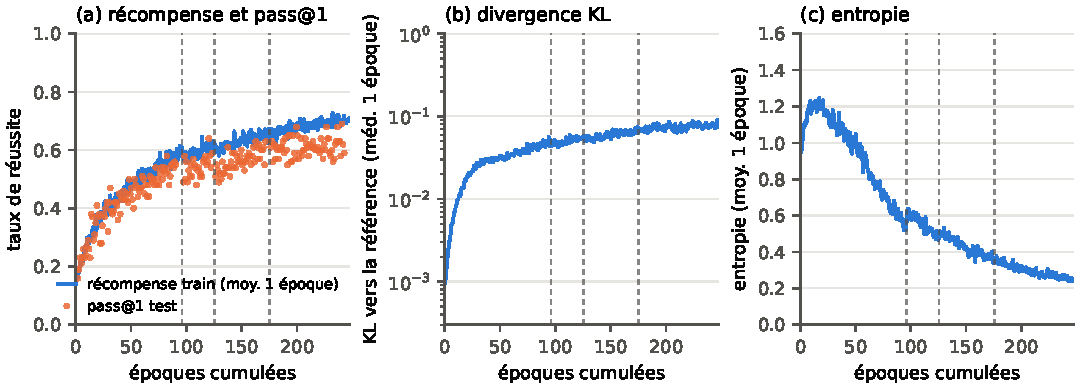
\includegraphics[width=\textwidth]{figures/fig_fullft_stabilite.pdf}
    \caption{\textsc{Replication-FT} lineage over 247 cumulative epochs, four segments separated by the vertical lines (each segment resumes from the best or the last checkpoint of the previous one). (a) Training reward averaged over one epoch and test pass@$1$ at each evaluation, on the same scale. (b) KL divergence toward the fixed reference, median over one epoch, logarithmic scale. (c) Policy entropy, mean over one epoch. Almost monotonic rise, bounded KL, slowly decreasing entropy: no collapse over the whole duration.}
    \label{fig:fullft_stabilite}
\end{figure}







\subsubsection{LoRA: Motivation, Grid and Diagnosis}

\paragraph{Why LoRA.} The previous lineage set the reference, but at a cost that ruled out the rest of the program: at some sixty hours per 72 epochs, the planned curriculum campaign would not have fit within the internship. Low-rank adaptation~\cite{hu2022lora} trains only small additive matrices, which divides the optimizer memory and the checkpoint size by a factor between fifty and eighty depending on the measure: 120~MB of optimizer state and 180~MB per best model at rank 8, against 8~GB and 14~GB in \emph{full fine-tuning}. This saving has three uses in what follows. It makes resumptions after a purge almost free. It frees GPU memory for the generation engine, which will make it possible to double the size of the GRPO groups (Section~4.3). And it allows grids of experiments that \emph{full fine-tuning} made impossible on a single GPU.

The blog post \emph{LoRA Without Regret}~\cite{schulman2025lora} provided a second, scientific motivation. Its authors observe that in RL, LoRA matches \emph{full fine-tuning} even at very small rank, and propose an explanation: a policy gradient algorithm would learn ``only about one bit of information per episode'', since a single reward scalar concludes each episode, so that a restricted parameter subspace would suffice to absorb it. They present this reading as a hypothesis, and support it with single-turn mathematical reasoning experiments with binary reward. They derive a recipe from it: a learning rate about ten times higher than that of \emph{full fine-tuning}, roughly independent of the rank. We wanted to know whether this recipe and this explanation held in our regime, which differs from theirs by being multi-turn, with long trajectories and interleaved observations.

\paragraph{The grid.} \textsc{LoRA-Grid} adopts the paper's recipe and changes only the adaptation: three ranks ($r \in \{16, 32, 64\}$, $\alpha = 32$), two learning rates ($10^{-5}$, the blog's prediction, and $3 \times 10^{-6}$) and two values of $\beta$ ($10^{-3}$ and $10^{-2}$), always toward a fixed reference. Six of the nine configurations were run; the other three, predictable in light of the first ones, were abandoned. The landscape offers no satisfactory operating region.

\begin{itemize}
    \item The blog's learning rate causes a fast and complete collapse: peak at 24\,\% around the third epoch, then 0\,\%.
    \item At $3 \times 10^{-6}$ and $\beta = 10^{-3}$, the rise is the fastest, 31 to 35\,\% depending on the rank, above the \emph{full fine-tuning} reference at equal budget (30 to 32\,\% at epoch 15), then every run collapses in its second half.
    \item At $3 \times 10^{-6}$ and $\beta = 10^{-2}$, $r=64$ plateaus between 21 and 29\,\% without collapsing; $r=16$ reaches 39\,\% then drops to 10\,\% around the twelfth epoch before partially recovering.
    \item Rank rescues nothing, and the relationship runs counter to the capacity intuition: at equal hyperparameters, $r=16$ does better than $r=32$, which does better than $r=64$.
\end{itemize}

\paragraph{Diagnosis.} The KL divergence toward the reference makes this landscape legible (Figure~\ref{fig:kl_lora_vs_fullft}). All runs start at the same level, $10^{-3}$, the drift of a single optimization step. \emph{Full fine-tuning} then moves away from it steadily, by about $10^{-3}$ per epoch over the window of the figure, then ten times more slowly beyond the thirtieth epoch (Figure~\ref{fig:fullft_stabilite}). The fixed-reference LoRA runs move away from it geometrically: from the fourth epoch on, their KL is multiplied by five to ten every two epochs, faster for larger ranks and later for stronger $\beta$. All cross the same level, between 0.05 and 0.1, and exceed 1 within the following four epochs; none recovered. This level is in no way absolute: \emph{full fine-tuning} settles there after thirty epochs without harm, and the moving-reference runs that follow sometimes exceed it transiently before being pulled back to it. What makes it fatal here is the dynamics by which it is reached, a geometric growth that nothing slows down. 





An order of magnitude explains why $\beta$ cannot prevent it. The policy term of the loss is about $3 \times 10^{-3}$ on a healthy run. At KL $= 10^{-3}$ and $\beta = 10^{-2}$, the penalty is $10^{-5}$, three hundred times smaller: it is inert in the healthy regime, which is desirable. It becomes comparable to the policy term only around KL $= 0.3$, when the geometric growth is already under way. The brake therefore engages only once the drift is irreversible, and a value of $\beta$ ten times stronger would cap scores that $\beta = 10^{-2}$ already caps.

It remains to explain why LoRA drifts faster than \emph{full fine-tuning} at equal progress. We have no established answer, and propose two hypotheses.

\begin{itemize}
    \item \textbf{Product parameterization.} The weight increment is written $BA$, and the gradient of each factor is proportional to the other. The blog's authors invoke this optimization dynamic, ``less favorable than that of the full matrix'', to explain that LoRA tolerates large batches poorly in supervised learning. Our rollout batch of 256 trajectories and our four steps per rollout batch place the grid in this regime; the hypothesis is that the same coupling amplifies each step in RL.
    \item \textbf{Signal noise.} A binary and sparse reward produces noisy gradients. \emph{Full fine-tuning} spreads them over billions of parameters, where they partly cancel out; LoRA concentrates them on a few matrices, where they accumulate. This is our hypothesis, not the blog's, and it has not been tested in isolation.
\end{itemize}

Whatever the cause, the consequence is the same: at equal progress, the LoRA policy moves away from its reference faster, and the pull toward a fixed reference is either too weak to prevent the runaway, or strong enough to prevent it but at the price of a ceiling. This diagnosis points to the fix of the next subsection. Let us finally note that the rank $r=8$ adopted thereafter extends the trend of the grid without having been compared with the other ranks under a moving anchor; we count it among the uncontrolled variables of the study.

\begin{figure}[htbp]
    \centering
    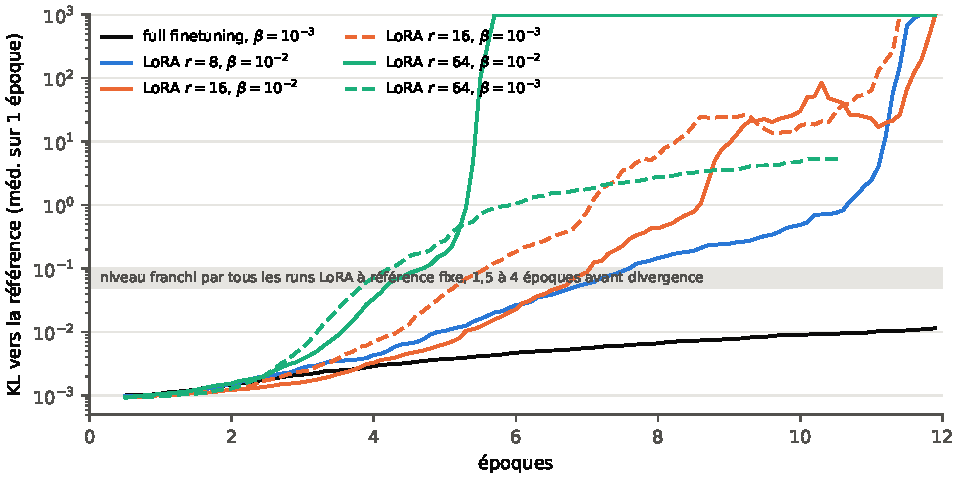
\includegraphics[width=0.9\textwidth]{figures/fig_kl_lora_vs_fullft.pdf}
    \caption{KL divergence toward the fixed reference during the first twelve epochs, rolling median over one epoch, logarithmic scale. \emph{Full fine-tuning} drifts linearly; all LoRA runs drift geometrically, faster for larger ranks (color) and later for stronger $\beta$ (solid line $10^{-2}$, dashes $10^{-3}$). The gray band marks the level crossed by all fixed-reference LoRA runs one to four epochs before their divergence; \emph{full fine-tuning} reaches it after thirty epochs without harm.}
    \label{fig:kl_lora_vs_fullft}
\end{figure}









\subsubsection{The Moving KL Anchor: Fix and Crossed Experiment}

\paragraph{Principle.} The preceding diagnosis locks the fixed reference in a dilemma: a weak pull lets the drift run away, a strong pull prevents it but caps the scores. In both cases, the defect is the same: the KL penalty measures the distance to an ever more distant point, the base model, and pulls the policy backward, against its progress. The way out of the dilemma consists in moving the reference. Our moving KL anchor proceeds by periodic merge-and-restart: every four epochs, the current adapter is merged into the model's weights, a fresh adapter replaces it, the KL penalty is henceforth measured toward this new point, and the optimizer state of the LoRA parameters is reset to zero. The policy is unchanged at the moment of re-anchoring; only the reference point of the penalty moves. The nature of the pull then changes: instead of holding the policy near its starting point, it holds it near its state of a few epochs ago, and penalizes only fast drift. We identified after the fact that this mechanism, merging the adapter then restarting a fresh adapter, is that of ReLoRA~\cite{lialin2023relora}. It has two properties that the name ``moving anchor'' obscures. After $k$ cycles, the weight increment is a sum of $k$ rank-8 products, hence of rank up to $8k$: the method accumulates capacity. And the optimizer state is reset to zero at each cycle. The moving reference, the accumulated capacity and the optimizer purge are therefore confounded in all our moving-anchor runs; separating them requires a live adapter that is never reinitialized and a frozen copy of the policy as reference, which the library does not allow without modification (Section~5).

This mechanism echoes an old idea from deep RL. TRPO~\cite{schulman2015trpo} constrained each update to remain, in KL divergence, within a trust region around the previous policy; PPO~\cite{schulman2017proximal} replaced this constraint with clipping of the importance ratio (Appendix~A). A KL penalty toward a recent reference is a soft form of the same idea, at the scale of a few epochs rather than of a single step. We designed it from our own curves, then found it in the literature: ProRL~\cite{liu2025prorl} periodically resets its reference policy ``to a recent snapshot of the online policy'' and reinitializes the optimizer, because ``the KL term eventually dominates the loss and blocks updates''. In ProRL the trigger is validation stagnation; in our case the period is fixed. Let us finally specify the origin of the choice: it is not a mathematical constraint but an implementation limit. TRL refuses to synchronize the reference on a PEFT model, the reference being the base model without adapter; merging followed by a restart is the least invasive modification that actually moves the reference.

\paragraph{Results.} The \textsc{Moving-Anchor} configuration ($r=8$, $\beta=10^{-2}$, re-anchoring every 4 epochs) rises from 12 to 35\,\% in 15 epochs without incident, where the best fixed-reference configurations have already reached their peak and started to fall back (Figure~\ref{fig:anchor_square}a). Continued, it reaches 65\,\% around the hundredth epoch after 25 re-anchorings; resumed from that point for sixty additional epochs, it reaches 73\,\%. No collapse over the whole lineage. Panel (b) of the figure gives the reason: the KL toward the reference stays at $10^{-3}$ throughout, with a sawtooth at each re-anchoring, whereas, for the fixed-reference runs, it runs away between the fifth and eighth epochs.

The \textsc{Anchor-Square} crossed experiment supports two conclusions. First, the moving anchor is necessary in our regime: with a fixed reference, the KL diverges whatever the value of $\beta$, between the fifth and eighth epochs, and no run progressed any further afterwards; the score collapses, or freezes when the policy, having become deterministic, keeps solving the same tasks (Figure~\ref{fig:anchor_square}a and~b). Second, the crossed experiment removes a confounding factor from the grid: $\beta = 10^{-3}$, whose KL diverged with a fixed reference, stays at a KL of $10^{-3}$ with a moving reference, and the run is stable at 53\,\% after 60 epochs. It is therefore the reference regime, and not the value of $\beta$, that governs stability. The two values of $\beta$ are moreover indistinguishable with a moving reference: between epochs 49 and 58, the evaluations average 48.9\,\% for $\beta=10^{-2}$ and 49.7\,\% for $\beta=10^{-3}$. The final gap, 65 then 73 against 53, is due to the duration of the runs, the second having been stopped at epoch 60. We kept $\beta=10^{-2}$ for what follows by continuity of lineage, not because it is better.

\paragraph{Scope.} This recipe carried our model above the published score, but we claim neither that it is universal nor that it is the best. It was developed on a single environment, with a rank and a re-anchoring period chosen without a grid. Its robustness remains to be established on the other AgentGym-RL environments, for which the platform provides the infrastructure. It does, on the other hand, have an immediate benefit already noted: the memory freed by LoRA made it possible, in the next phase, to double the size of the GRPO groups at a constant number of trajectories, hence to estimate the advantage of each task over 16 trajectories instead of 8.



\begin{figure}[htbp]
    \centering
    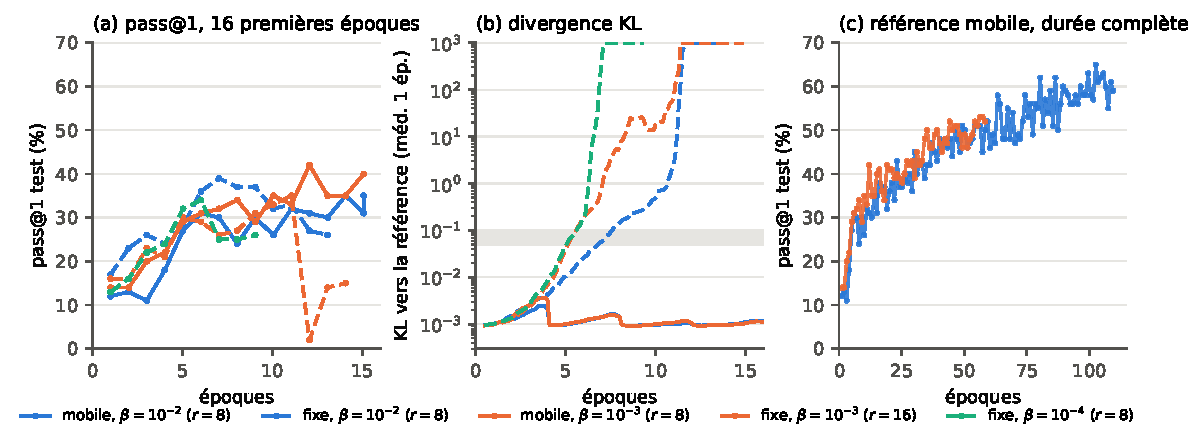
\includegraphics[width=\textwidth]{figures/fig_anchor_square.pdf}
    \caption{Crossed design, fixed or moving reference $\times$ $\beta$ (color: $\beta$; dashes: fixed reference; solid line: moving reference). (a) Test pass@$1$ over the first sixteen epochs: the fixed-reference runs reach their peak between the sixth and eleventh epochs then collapse, faster for weaker $\beta$; the moving-reference runs rise without incident. (b) KL divergence toward the reference, median over one epoch, logarithmic scale: the three fixed-reference runs cross the gray band between the fifth and eighth epochs then diverge; the moving-reference runs stay at $10^{-3}$, with a sawtooth at each re-anchoring. (c) Test pass@$1$ of the two moving-reference runs over their whole duration: 65\,\% around epoch 100 for $\beta=10^{-2}$, 53\,\% at the voluntary stop at epoch 60 for $\beta=10^{-3}$.}
    \label{fig:anchor_square}
\end{figure}






\subsubsection{Precursor Signals and Summary}

\paragraph{Two collapse modes.} We have fifteen runs of more than five epochs on the current stack: six stable over their duration, six fixed-reference collapses, and three collapses at $G=16$ without curriculum, detailed in Section~4.3. Their hyperparameters differ, which forbids any causal reading; but the entropy and KL trajectories cluster into two clear signatures (Figure~\ref{fig:collapse_signals}). We first recall the empirical result of Cui et al.~\cite{cui2025entropy} that serves as our interpretive framework: in RL with verifiable reward, the policy's entropy decreases as performance rises, performance ``is paid for in entropy'', and when the entropy approaches zero the policy becomes deterministic, exploration dies out and learning stops.

\begin{itemize}
    \item \textbf{With a fixed reference, the KL goes first.} From the fourth epoch on, the median KL grows geometrically (Section~4.2.3) while the entropy remains high, and even rises to 1.4 or 1.5: the policy becomes more erratic, not more deterministic. Between the fifth and eleventh epochs, the KL exceeds 1 and the entropy collapses at the same moment, in less than one epoch. The policy is then either destroyed or frozen.
    \item \textbf{With a moving reference and $G=16$ without curriculum, the entropy decreases, then the KL jumps.} On \textsc{Control-G16}, the KL stays at $10^{-3}$, brought back at each re-anchoring, while the entropy decreases steadily, from 1.1 toward 0.6 in six to eight epochs. Then, in less than one epoch, the entropy falls below 0.2 and the KL jumps from $10^{-3}$ to more than $10^{8}$. This is the entropy collapse of Cui et al., which the moving anchor cannot see coming: by re-basing itself on a policy that is becoming deterministic, it validates the degeneration instead of slowing it. This order is not general: the two other controls without curriculum at $G=16$, re-anchored every twelve then every eight epochs, diverge through the KL before their entropy collapses. The token-by-token replay of a checkpoint from the collapse (Appendix~F.7) gives its mechanism. The per-token KL estimator, $k_3 = e^{\rho} - \rho - 1$ with $\rho = \log \pi_{\mathrm{ref}} - \log \pi$, is not bounded in TRL, whereas the paper's code bounds it to $[-10, 10]$. A sharpened policy drops a few tokens that the reference expected with probability close to 1: on such a token, $\rho$ reaches 5 then 18, and $k_3$ amounts to $10^{2}$ to $10^{8}$. The gradient of the update is then dominated by this single token, the format breaks, turns loop until truncation, and the end marker forced on these turns ($\rho \approx 45$) carries one hundred percent of the measured KL, at $10^{19}$ per token. The log-probability gap between the generation engine and the recomputation during backpropagation is not to blame: its median is $10^{-5}$ nat. Section~4.3 proposes the mechanism of the entropy decrease that precedes it.
\end{itemize}

A third case sheds light on the first two. The \textsc{Control-G16} run relaunched with re-anchoring every twelve epochs follows the first signature, not the second: without re-anchoring before epoch 12, it behaves like a fixed reference, and its KL diverges from the fifth epoch on. A second control, with eight tasks of sixteen trajectories and re-anchoring every eight epochs, i.e. the same number of steps between two anchors as the control, also diverges through the KL, at the fifteenth epoch (Appendix~F.6). Figure~\ref{fig:collapse_signals}b moreover shows that all runs at $G=16$, stable or not, drift quickly during their first four epochs, up to a KL of 0.1 or 0.3: it is the re-anchoring of the fourth epoch that brings them back to $10^{-3}$. Spacing out the re-anchorings is therefore not an option in this regime.

\paragraph{Verification by the bound.} One run resumes \textsc{Control-G16} identically, with the sole difference that $k_3$ is bounded at 10 per token, as in the paper's code (\textsc{Control-G16-Bounded}). It passes through epochs 10 and 15, where the two previous controls were dead, without any loop or KL jump, and continues its rise over 80 epochs, resumed from the saved checkpoint after an infrastructure interruption at epoch 58; its best score is 82\,\% and its plateau 76. The link ``unbounded estimator, hence divergence'' is thus confirmed. The bound does not protect entropy, quite the contrary: it falls to 0.11 as early as the fourth epoch, against 1.0 for the unbounded control at the same point, because bounding $k_3$ cancels the gradient of the penalty on the tokens where the policy has moved furthest away, and nothing then slows the sharpening any longer. The run then lives at an entropy between 0.2 and 0.3, with turns of a dozen tokens and no written reasoning; its score nevertheless matches that of the horizon curriculum at the same number of updates (Section~4.3.2).

\paragraph{Limits of the signal analysis.} Two metrics accompany the collapse without preceding it. Generation length crashes at the moment of collapse, below 250 tokens of stereotyped outputs, then explodes in some runs, up to several thousand tokens of degenerate text. The training reward, for its part, gives no warning: on \textsc{Control-G16}, it holds at 0.5 during the two epochs where the KL is already $10^{8}$, because a deterministic policy keeps solving the tasks it knows. The two usable precursor signals are therefore the geometric growth of the KL with a fixed reference, and the steady decrease of the entropy with a moving reference. We did not carry out a systematic correlation analysis between these signals, the error classes and the moment of collapse; it is an analysis directly feasible on our logs, which we leave as future work.

\paragraph{Learning-rate regulation.} Before the moving anchor, we sought stability in the regulation of the learning rate, on a lineage of fixed-reference LoRA runs. Scheduled stages stabilize but interrupt progressions under way. An adaptive cut, triggered on stagnation of the training reward, often triggers on noise; above all, cutting the rate consolidates the current state, which after a peak is often already a drift. The healthiest variant combines long stages and restoration of the best state of the elapsed stage. These mechanisms and the policy of keeping the best checkpoints with their optimizer are described in Appendix~C. The final recipe no longer needs them: at a constant rate, the moving anchor suffices.

\paragraph{Section summary.} This section established the conditions under which multi-turn GRPO training progresses without collapsing, and verified them on our runs. The gradient is correct only if the observations are kept in the sequence and masked; without this, the model does not learn and nothing signals it. A reward term added to densify the signal was optimized for its own sake: the policy learned to give up on long tasks, and we kept the binary reward. The paper's recipe in \emph{full fine-tuning} is stable over 247 epochs and reaches 69\,\%, at a cost in time and memory that ruled out the rest. LoRA removes this cost but drifts geometrically in KL toward a fixed reference, whatever the rank and coefficient tested. Moving the reference every four epochs removes the drift and carries the same model to 73\,\%. Finally, the analysis of fifteen runs distinguishes two collapse modes, one through the KL with a fixed reference, the other through the entropy at large group size. The moving anchor settles the first. The second is due to a defect of the KL estimator, unbounded in our library whereas the paper's code bounds it; the bound removes the divergence. What it does not settle, entropy exhaustion and the resulting plateau, is the subject of the next section.

\begin{figure}[htbp]
    \centering
    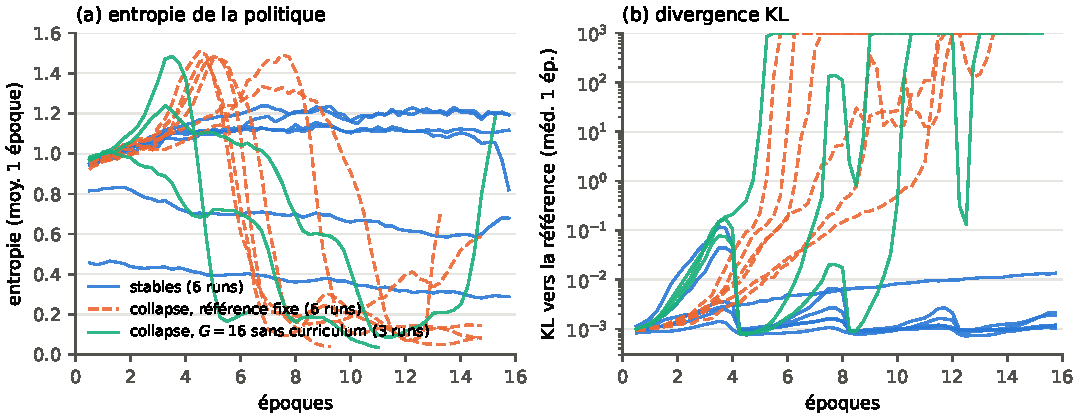
\includegraphics[width=\textwidth]{figures/fig_collapse_signals.pdf}
    \caption{First sixteen epochs of fifteen runs, grouped by outcome: stable over their duration (blue), fixed-reference collapse (orange, dashes), collapse at $G=16$ without curriculum (green). (a) Policy entropy, mean over one epoch: with a fixed reference, it rises to 1.4 or 1.5 before collapsing all at once; at $G=16$ with re-anchoring every four epochs, it decreases steadily for six to eight epochs before collapsing; the controls re-anchored less often diverge first through the KL. (b) KL divergence toward the reference, median over one epoch, logarithmic scale: geometric growth with a fixed reference; with a moving reference, fast drift during the first four epochs then return to $10^{-3}$ at each re-anchoring (sawtooth), except for the run re-anchored every twelve epochs, which diverges from the fifth on.}
    \label{fig:collapse_signals}
\end{figure}


















\vspace{2cm}


\subsection{RL Experiments: The Curricula}
\label{sec:curriculums}

Section~4.2 left a question open. The moving KL anchor suppresses the drift of the policy away from its reference, but it does not see the second mode of collapse: the one in which entropy is progressively exhausted, at stable KL, until the policy becomes deterministic. The curriculum is the first candidate for addressing it, and it is in this capacity that we first studied it.

It lends itself, however, to a twofold reading, and this duality is the central idea of the section. On one side, the curriculum is an optimization tool: a way of calibrating the difficulty presented to the policy so that it learns faster, higher, or more reliably. On the other, it touches on more open research questions, those of exploration and meta-learning: can the structure of experience make a policy exceed what its base model already knew how to do? Does what is acquired at one difficulty transfer to the others? Does the order of presentation change the way of learning, the speed at which each depth is acquired, generalization, the order in which errors disappear? These questions are riskier than the first, and we do not claim to settle them with three runs. But they justify the interest in the curriculum beyond its role as a stabilizer: at worst, it stabilizes; at best, it learns differently.

The section unfolds in three stages. Section~4.3.1 describes three curriculum regimes compared under an identical training recipe, against two references without curriculum. Section~4.3.2 presents their results and the reading they allow, including the role of the curriculum in stability. Section~4.3.3 proposes a mechanism, at the level of the gradient, that accounts both for the collapse without curriculum and for the protection the curriculum provides. The compute-controlled comparison of the regimes is the subject of Section~4.4. The transfer between single-turn planning and interactive control, initially planned here, could not be carried beyond preliminary measurements; it is presented in Section~4.5 and taken up again in the outlook as a form of meta-learning.





\subsubsection{Three Curriculum Regimes Under a Common Recipe}

\paragraph{What a curriculum is.} In its initial formulation, \emph{curriculum learning} presents training examples in order of increasing difficulty~\cite{bengio2009curriculum}. In reinforcement learning, the notion has broadened: the survey by Narvekar et al.~\cite{narvekar2020curriculum} defines a curriculum as a sequence of tasks, or of samples, organized to learn a target problem, and that of Portelas et al.~\cite{portelas2020acl} describes automatic curriculum methods as mechanisms ``that shape the learning trajectory of an agent by proposing tasks adapted to its capabilities''. Two levers are therefore possible. The first orders the tasks: which tasks to present, and when. The second acts on the means granted to the agent to solve a given task: how many turns, how many tokens. ScalingInter~\cite{xi_agentgym-rl_2025} falls under this second lever, which is still little explored. The regimes below cover both.

\paragraph{Common recipe and references.} The three regimes share the recipe stabilized in Section~4.2: LoRA of rank 8, learning rate $3 \times 10^{-6}$, $\beta = 10^{-2}$, moving anchor every 4 epochs, groups of $G=16$ trajectories and 64 trajectories per update, final horizon of 30 turns, 80 epochs planned. They are compared against two references without curriculum. \textsc{Moving-Anchor} is the reference at $G=8$, 65 then 73\,\%. \textsc{Control-G16} applies the common recipe identically, without curriculum: it is the control that isolates the effect of the curriculum. Note that at 64 trajectories per update, moving from $G=8$ to $G=16$ also halves the number of tasks seen per update, from eight to four; the two effects are not separated in our runs. It did not hold, and this collapse is one of the results of the next section. In accordance with the protocol, each configuration is a single run and no hyperparameter was tuned separately for any regime: the conclusions are conditional on this common recipe.

\begin{itemize}
    \item \textbf{\textsc{Horizon}: the number of turns.} This regime adopts the principle of ScalingInter: the maximum number of interaction turns per episode is 10 from epoch 0 to 15, 20 from epoch 15 to 30, then 30. The hypothesis is as follows. A low cap lets only those tasks succeed that can be solved in few turns: the easiest ones, and the medium tasks provided they are solved without detours. It therefore first forces efficiency on short tasks, and makes long tasks temporarily unsolvable; each raising of the cap reintroduces them. The success curves by depth (Section~4.3.2) will allow this reading to be checked. Our schedule is slower than that of the paper, whose scripts change stage every 100 updates, that is, roughly every two epochs in their configuration; we preferred long stages, to let each level saturate before moving on to the next.
    \item \textbf{\textsc{Budget}: the number of tokens per turn.} This regime transposes the same idea to the length of the agent's responses: 256 tokens per turn from epoch 0 to 15, 512 from epoch 15 to 35, then 1\,024, the horizon remaining fixed at 30 turns. A short budget forbids long reasoning and degenerate outputs; raising it then allows more elaborate turns. It is a direct extension of ScalingInter to a second parameter of the harness.
    \item \textbf{\textsc{Depth}: the structure of the tasks.} This regime is the closest to the original definition: it orders the tasks without touching the agent's means. Sampling is uniform over the recipes of depth less than or equal to the current stage, and the stage rises from 1 to 4. The mechanism is a weighted sampler over the whole set of recipes, not a partition into subsets: the definition of epochs and the rest of the training loop are identical to the other regimes. A first version fixed the stages on a schedule, at epochs 0, 12, 25 and 37. It showed that a stage held too long saturates: on stage 1, the training reward reaches 1 from the sixth epoch onward, all groups become uniform and the gradient is zero for six epochs. The second version makes the transition adaptive: the stage rises as soon as the mean training reward exceeds 0.8 over a full epoch, or at the latest after 10 epochs.
\end{itemize}

These three regimes set the difficulty by hand, according to a notion of difficulty that is our own: the number of turns, the length of responses, the depth of recipes. Nothing guarantees that it coincides with the effective difficulty for the model, and in a real environment, recommendation for instance, this difficulty is not even known in advance. An automatic curriculum, which selects tasks according to the progress the model makes on them, addresses this limitation; we ported and ran one instance of it, presented in Section~4.5 with the exploratory directions. Finally, these regimes each act on a single lever; their combination has not been tested, and figures among the most direct extensions of this work (Section~5).






\subsubsection{Results: the Curriculum as a Condition of Stability at $G=16$}

\paragraph{The control first.} \textsc{Control-G16} applies the common recipe without curriculum. It rises quickly, from 12 to 54\,\% in thirteen epochs, faster than the reference at $G=8$ at an equal number of trajectories (Figure~\ref{fig:curricula_main}a). Then it collapses according to the second signature of Section~4.2.5: the entropy of the policy decreases steadily from 1.0 to 0.6 between the third and the tenth epoch, the KL divergence remaining at $10^{-3}$, then both tip over in less than an epoch, entropy below 0.15 and KL beyond $10^{8}$. The test score falls back from 54 to 13\,\% and the generations degenerate. A second attempt with re-anchoring every twelve epochs instead of four diverged even earlier, from the fifth epoch, for lack of re-anchoring before the twelfth. We did not pursue further: this collapse is in itself the result, the one against which the three curricula are compared.

\paragraph{The three curricula.} Under an identical recipe, the three regimes cross the zone where the control collapses and continue their rise over 80 epochs (Figure~\ref{fig:curricula_main}a). \textsc{Horizon} reaches 82\,\% twice, at epochs 65 and 77, and ends on a plateau whose last ten evaluations average 78\,\%, between 75 and 82; it goes through twenty re-anchorings. \textsc{Budget} reaches 78\,\% at epoch 55, then 80\,\% after a resumption, on a plateau at 75\,\%. \textsc{Depth}, in its adaptive version, reaches 72\,\% at epoch 43, then 80\,\% after a resumption, on a plateau at 74\,\%. The two resumptions were imposed by purges of the compute environment and are described in Appendix~C. The three curves are almost superimposed over the whole duration; \textsc{Horizon} pulls slightly ahead at the end of the run. They dominate the \textsc{Moving-Anchor} reference at $G=8$, which reaches 73\,\% at the end of 170 epochs, i.e. a 70\,\% plateau, at an equal number of updates. Recall the scale: the \emph{full fine-tuning} lineage had required about 247 epochs to reach 69\,\%.

\paragraph{Reading.} These runs deliver the central reading of the section. Under a common recipe, doubling the group size speeds up learning per epoch, but not at an equal number of trajectories: the two runs that differ only in $G$, at eight tasks per step, stand at 50 and 60\,\% after 180\,000 trajectories, in favor of $G=8$ (Appendix~F.6). What $G=16$ unquestionably speeds up is the policy becoming deterministic: without curriculum, the recipe is unstable at this speed. With a curriculum, whatever its lever, it does not become so. The curriculum is therefore not only an accelerator; it is, in this regime, a condition of stability. Figure~\ref{fig:curricula_main}b clarifies the role it plays. It does not prevent entropy from decreasing: that of \textsc{Horizon} goes from 0.8 to 0.2 in 80 epochs, those of \textsc{Budget} and \textsc{Depth} follow the same slope. It prevents its abrupt collapse, the one which, on the control, precedes the divergence of the KL. Section~4.3.3 proposes the mechanism of this protection. It is not the only one: the bound on the KL estimator suffices to avoid the divergence (Section~4.2.5). What distinguishes the curriculum is visible over the long run. At an equal number of trajectories, curricula and stabilized controls are indistinguishable up to 120\,000 trajectories, between 55 and 58\,\%; beyond that, the curricula continue toward 75 to 80 while the runs without curriculum plateau between 60 and 72. The difference is not the initial speed, it is the plateau. The bounded control, at 73\,\% at epoch 57 against 74 for \textsc{Horizon} at the same point, but at an entropy of 0.2 against 0.3 to 0.6, was at the bifurcation point; continued to 80 epochs, it reaches the same plateau, and Appendix~F.8 examines what is then left to the curriculum: its cost and its entropy. This finding remains conditional: one run per configuration, no regime-specific tuning, and only two attempts for the control.

\paragraph{Order of acquisition and elimination of errors.} Two analyses drawn from the periodic evaluations complete the picture. The first stratifies pass@$1$ by depth (Figure~\ref{fig:acquisition_depths}). The order of acquisition is the same in all regimes, curriculum or not: depth 1 is acquired in under five epochs, depth 2 exceeds 80\,\% around the thirtieth and reaches 90\,\% around the sixtieth, depth 3 progresses slowly up to 30 or 45\,\%, and depth 4 stays at zero. The curricula did not change this order; they accelerated each step relative to the reference at $G=8$. The depth curriculum, which explicitly presents deep recipes last, does no better than the others on depth 3. The second analysis tracks the error classes returned by the environment (Figure~\ref{fig:elimination_erreurs}). Format errors, malformed action or several actions in one turn, disappear in under ten epochs in all regimes; they are the ones that reappear en masse during the collapse of the control. Planning errors, invalid recipe, missing ingredient or item not found, decrease slowly over the whole duration, from twelve to five per episode for \textsc{Horizon} and \textsc{Depth}, from twelve to seven for \textsc{Budget} and the reference. RL therefore first corrects the form, then, much more slowly, the substance; the curriculum accelerates both without changing their order.

\begin{figure}[htbp]
    \centering
    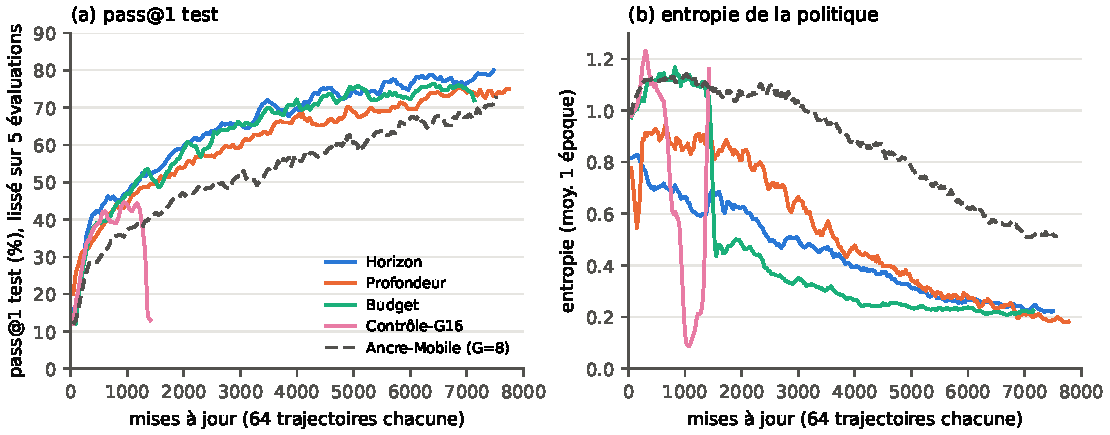
\includegraphics[width=\textwidth]{figures/fig_curricula_pass1_entropy.pdf}
    \caption{Three curricula (\textsc{Horizon}, \textsc{Depth}, \textsc{Budget}), the control without curriculum at $G=16$ and the reference at $G=8$, as a function of the number of updates, each of 64 trajectories. (a) Test pass@$1$, smoothed over five evaluations. (b) Entropy of the policy, averaged over one epoch. The \textsc{Depth}, \textsc{Budget} and $G=8$ lineages include a resumption after a purge (Appendix~C). The control collapses around the thousandth update; the three curricula continue their rise.}
    \label{fig:curricula_main}
\end{figure}

\begin{figure}[htbp]
    \centering
    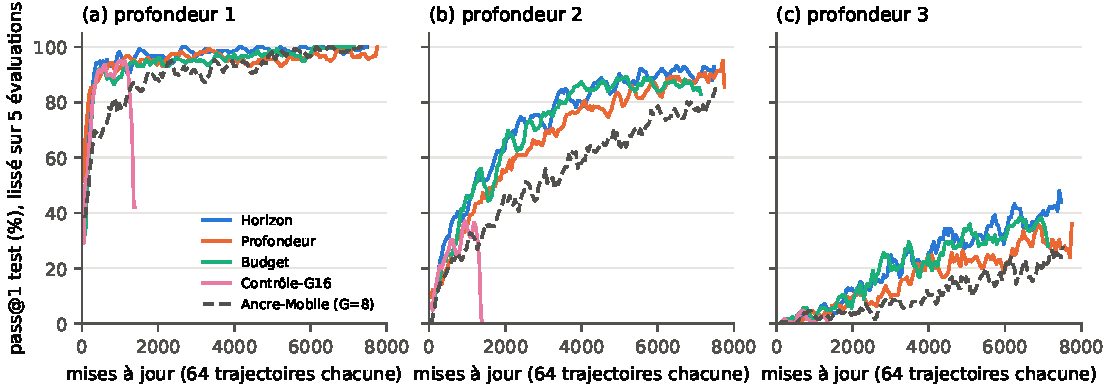
\includegraphics[width=\textwidth]{figures/fig_curricula_depths.pdf}
    \caption{Test pass@$1$ by recipe depth, smoothed over five evaluations, for the same runs. Depth 4 (three test tasks, a single one in training) stays at zero in all regimes and is not plotted. The order of acquisition is identical everywhere: depth 1, then 2, then 3; the curricula accelerate it without changing it.}
    \label{fig:acquisition_depths}
\end{figure}

\begin{figure}[htbp]
    \centering
    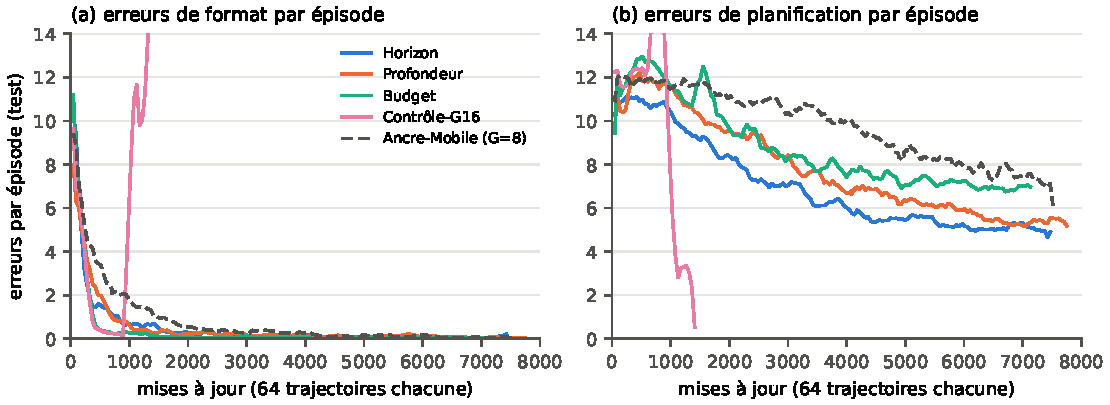
\includegraphics[width=\textwidth]{figures/fig_curricula_errors.pdf}
    \caption{Mean number of errors per test episode, smoothed over five evaluations. (a) Format errors: malformed action, several actions in one turn, misspelled item name. (b) Planning errors: invalid recipe, insufficient ingredients, item not found. Format errors disappear in under a thousand updates in all regimes and reappear during the collapse of the control; planning errors decrease slowly over the whole duration.}
    \label{fig:elimination_erreurs}
\end{figure}



\subsubsection{Mechanism: What Produces Gradient}

Why does training without curriculum collapse at large group size, and why does the curriculum protect it from doing so? We propose a mechanism at the level of the gradient. It is consistent with all our curves, but two of its links have not been measured directly; we present it as a hypothesis.

\paragraph{The starting point.} Cui et al.~\cite{cui2025entropy} establish that the change in entropy of a softmax policy, at each learning step, is driven by the covariance between the probability of an action and the change in its logits; under a policy gradient, this change is proportional to the advantage of the action. Entropy therefore decreases when already-probable actions receive a positive advantage and improbable actions a negative one; it increases in the opposite case. The authors further observe an empirical law, $R = -a\,e^{H} + b$, linking performance to entropy: the attainable performance is capped by the exhaustion of entropy. Everything therefore hinges on which actions are rewarded and which are punished, not on the level of the reward.


\paragraph{What produces gradient.} In GRPO, the advantage is computed per task, over the group of $G$ trajectories from the same prompt. A group that is entirely successful or entirely failed has zero advantage and produces no gradient. Only mixed groups produce any. Controlling learning therefore means controlling which items are mixed, and when.

\paragraph{Without curriculum, the configuration has the wrong sign.} The base model has support on the hard tasks: at thirty turns, a depth-3 recipe typically yields one to three successes out of sixteen. The group is mixed and produces gradient. But the success is short and made of routine, hence probable, actions: it receives a strongly positive advantage, of the order of $+3.9$ for one success out of sixteen. The fifteen failures last thirty turns and fill up with drift, with improbable actions, and the negative advantage applies to each of their tokens, since credit is assigned to the whole trajectory. Positive advantage on the probable, negative on the improbable: entropy decreases at every step, on dozens of tasks at once. The signal is correct, the model learns, even faster than with a curriculum at the same number of updates. But entropy is a finite resource: each mixed group with long failures consumes some, and nothing replenishes it. Around 0.1, the policy is deterministic, and any update then makes the KL divergence blow up. This is exactly the second signature of Section~4.2.5.

\paragraph{What the horizon curriculum changes.} The ten-turn cap acts in two ways. First, it turns mixed groups with long failures into entirely failed groups: succeeding at a depth-3 recipe requires more than ten turns, so none of the sixteen trajectories succeeds, the advantage is zero, and the entropy of the policy on these tasks is preserved because no gradient touches it. Second, the only remaining mixed groups are tasks solvable in ten turns, whose failures are short and contain few improbable actions. At the next stage, the hard tasks become mixed again, but under better conditions, reliable building blocks and failures cut off at twenty turns, and their new successes come from actions the model rarely produced: crafting an intermediate item at the second turn, redoing a \texttt{get} after a \texttt{craft}, chaining more than two crafts. Positive advantage on the improbable: entropy rises again. The curriculum does not pick items by hand; it is the cap that decides which items are mixed and when. The same reasoning holds for the token budget, which cuts off long drifts, and for depth, which removes the hard tasks from sampling.

\paragraph{The corollary for $G=16$.} With sixteen trajectories instead of eight, the probability that a hard task contains at least one success is larger. Without curriculum, there are therefore more mixed groups with long failures from the start, more gradient of the wrong sign, and an earlier collapse: tenth epoch for the control at $G=16$, no collapse in 110 epochs at $G=8$. With a curriculum, these tasks are entirely failed no matter what, and $G=16$ no longer has this effect. The autocurriculum of Appendix~E, run at $G=16$ without a cap, collapsed at the seventh epoch, as this mechanism predicts. The control with bounded estimator (Section~4.2.5) confirms the entropy consumption predicted by this mechanism, faster still once the KL brake is lifted; it also shows that this consumption is not enough to destroy the policy. The destruction came from the estimator.

\paragraph{In terms of exploration and exploitation.} The mechanism can be summarized as follows. In a mixed group at thirty turns, the success is short and routine: this is exploitation, and it is reinforced. The fifteen failures are long and full of rare actions: this is exploration, and it is punished token by token, good actions included, because a single final reward, without a process model, does not distinguish within a failure the actions that were right. At every step, exploitation wins and entropy decreases; nothing recharges it. The curriculum does not change the direction of the signal; it chooses when each task is allowed to produce gradient: out-of-reach tasks are not punished, failures are short, and the successes of the next stage come from rare actions. It is a regulator of the exploration-exploitation trade-off, applied through task selection rather than through a term in the loss.


\paragraph{What remains to be measured.} One measurement has since been made: on the control, turn length drops from 65 to 30 tokens and written reasoning disappears before the divergence (Appendix~F.7). Two inexpensive checks remain to be done: the mean length of the control's failed trajectories against that of the horizon curriculum during its first stage; and the share of rare actions, crafting an intermediate or a \texttt{get} after a craft, in the successes just after a stage change. Until they are done, the mechanism remains a hypothesis illustrated by the entropy curves, not a law.



\subsection{Compute-Controlled Comparison}
\label{subsec:compute-controle}

Section~\ref{subsec:protocole} set the convention: each update consumes 64 trajectories, whatever the group size, and runs with different group sizes are compared in updates, never in epochs. This convention equalizes the number of trajectories, not the compute spent to produce them. Yet this is where the budget curricula gain their advantage: a cap of 10 turns or 256 tokens shortens the episodes, hence the generation time of each update. A comparison in updates underestimates this advantage. We measure it here with three indicators. The first is the number of tokens processed, prompt and trajectory included, accumulated over the run: trajectory generation dominates the time of each update, and this counter is its closest measure, independent of the hardware. The second is GPU time, the sum of update durations: it is the billed cost, the one a practitioner must budget for, but it depends on the hardware and the infrastructure. The third is the number of environment turns, that is, of calls to the simulator, which would become the primary cost in a real environment. It is not recorded during training; we estimate it from the periodic evaluations: the mean number of turns over the 100 test episodes, capped by the current horizon stage, multiplied by the 64 trajectories of each elapsed update. The estimator assumes that training episodes have, at a given moment, the same length as test episodes; it gives an order of magnitude, not a measurement.

\paragraph{Effect of group size on raw speed.} A dedicated benchmark, eight updates per configuration under fixed conditions, gives 57.1~s per update at $G=8$ in the historical memory setting, against 46.9~s at $G=16$ with the enlarged generation cache, i.e. 18\,\% less. The mechanism is prefix sharing: the sixteen trajectories of the same task reuse the cache of its prompt. Enlarging the cache further is counterproductive (61.5~s). This benchmark mixes two changes, group size and cache, and measures only a speed at fixed policy. The mean speed of a real run depends moreover on episode length, hence on the policy and on the curriculum regime, as Table~\ref{tab:compute} shows.

\begin{table}[htbp]
\centering
\caption{Cost of the main lineages, figures as of the freeze of September 3, except the bounded control (September 23). One update consumes 64 trajectories. GPU hours: sum of update durations, evaluations excluded. Tokens: processed by the model, prompt and trajectory included. Turns: estimated from the periodic evaluations (see text). Plateau: mean of the last ten evaluations.}
\label{tab:compute}
\footnotesize
\setlength{\tabcolsep}{4pt}
\begin{tabular}{l c r r r r c c}
\toprule
\textbf{Lineage} & $\boldsymbol{G}$ & \textbf{Updates} & \textbf{GPU h} & \textbf{Tokens ($10^9$)} & \textbf{Turns ($10^6$)} & \textbf{Best} & \textbf{Plateau} \\
\midrule
\textsc{Replication-FT} & 8 & 11\,564 & 238 & 0.87 & 12.4 & 69 & 61 \\
\textsc{Moving-Anchor} & 8 & 8\,018 & 70 & 0.62 & 8.6 & 73 & 70 \\
\textsc{Horizon} & 16 & 7\,518 & 48 & 0.45 & 6.3 & \textbf{82} & \textbf{78} \\
\textsc{Depth} & 16 & 7\,904 & 66 & 0.56 & 7.9 & 80 & 74 \\
\textsc{Budget} & 16 & 7\,194 & 51 & 0.43 & 7.2 & 80 & 75 \\
\textsc{Control-G16} & 16 & 1\,434 & 16 & 0.15 & 1.9 & 54 & collapse \\
\textsc{Control-G16-Bounded} & 16 & 7\,440 & 51 & 0.47 & 6.7 & \textbf{82} & 76 \\
\bottomrule
\end{tabular}
\end{table}

\paragraph{Reading.} Three observations emerge from the table and from Figure~\ref{fig:pass1-tokens}, which places each lineage on the axis of processed tokens.

\begin{itemize}
    \item \textbf{The budget curricula are the cheapest per update.} \textsc{Horizon} costs 23~s per update and \textsc{Budget} 26~s, against 39~s for the control with full horizon and budget from the start, and 30~s for \textsc{Depth}, which runs 30 turns from the start. Over 80 epochs, \textsc{Horizon} processed 0.45 billion tokens whereas \textsc{Depth} processed 0.56 for a plateau four points lower. In environment turns, \textsc{Horizon} consumes half as many as \emph{full fine-tuning} for a plateau seventeen points higher. The explanation is mechanical: the initial stages cut the episodes short.
    \item \textbf{At equal tokens, the three curricula dominate the two references.} At 0.4 billion tokens, \textsc{Horizon} and \textsc{Budget} are between 75 and 80\,\%, \textsc{Depth} around 68, the reference at $G=8$ around 55 and \emph{full fine-tuning} around 55 as well. \emph{Full fine-tuning} reaches its 61\,\% plateau after 0.87 billion tokens and 238 GPU hours; \textsc{Horizon} exceeds this level after 0.1 billion and some ten hours.
    \item \textbf{Speed or asymptote.} Over 80 epochs, the three curricula have a higher plateau than the reference at $G=8$ after 170 epochs, 74 to 78 against 70. They therefore reach higher, and faster. But the reference was still rising when it was stopped, and no run was continued to full saturation: we cannot say whether the asymptotes differ, only that the curricula get there earlier.
\end{itemize}

\paragraph{Effect of group size alone.} The pair \textsc{Moving-Anchor} at $G=8$ and \textsc{Control-G16} does not isolate it: at 64 trajectories per update, the latter sees only four tasks per update instead of eight. Three complementary runs, run after the freeze, do so (Appendix~F.6). At eight tasks per step and re-anchoring every eight epochs, $G=8$ reaches 64\,\% and $G=16$ collapses at the fifteenth epoch; with re-anchoring every four epochs, $G=16$ holds for 80 epochs and finishes at 72\,\%. Two readings emerge. Group size does not speed up learning at equal trajectories: at 180\,000 trajectories, $G=16$ stands at 50\,\% and $G=8$ at 60\,\%. And the re-anchoring period matters more than $G$: the same run at $G=8$ stands at 60\,\% with re-anchoring every eight epochs, against 49 for \textsc{Moving-Anchor} every four, at equal trajectories.



\begin{figure}[htbp]
    \centering
    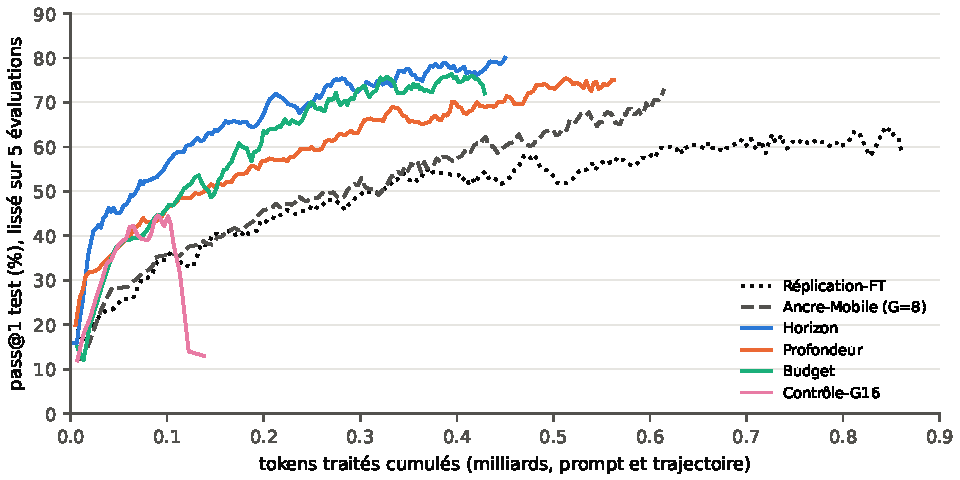
\includegraphics[width=0.95\textwidth]{figures/fig_pass1_tokens.pdf}
    \caption{Test pass@$1$, smoothed over five evaluations, as a function of the tokens processed cumulatively since the start of each lineage. At equal abscissa, the runs have consumed the same generation volume; the vertical gap measures the efficiency of each regime. The \textsc{Replication-FT}, \textsc{Moving-Anchor}, \textsc{Depth} and \textsc{Budget} lineages include resumptions after purges (Appendix~C).}
    \label{fig:pass1-tokens}
\end{figure}


\subsection{Complementary Experiments and Exploratory Directions}
\label{sec:inference_ablations}

The previous sections dealt with training. This one gathers three kinds of measurements that frame it. First, measurements without training: the pass@$k$ oracle, which puts the ceiling hypothesis stated in Section~2.3 to the test, the \emph{few-shot} prompt, and the comparison across model generations. Next, an experiment we were not able to redo in the stabilized configuration, the interaction between \emph{few-shot} prompting and RL. Finally, three exploratory directions, pursued on the margins of the central program and stopped before reaching a conclusion: trajectory recomposition by SNIS, transfer between single-turn planning and multi-turn control, and the MAGELLAN autocurriculum. Each is summarized here in one paragraph and developed in an appendix. Table~\ref{tab:recap_section4} recapitulates all the configurations of Section~4. Appendix~F gathers the complementary figures: the two other compute axes, episode length by depth, the fraction of groups without gradient, the effect of the stages on sequences, and the errors class by class.

\subsubsection{Pass@$k$ Oracle and the Ceiling Hypothesis}

Pass@$k$ is the fraction of tasks solved at least once in $k$ independent draws. For each of the 100 test tasks, our oracle draws twenty trajectories at temperature $1.0$ and at most 30 turns, then computes pass@$k$ for $k$ from 1 to 20 with the unbiased estimator of Chen et al.~\cite{chen2021codex}, overall and by depth. The resulting pass@$1$ is the mean over twenty passes; it is the reference retained for the untrained model in Section~4.1.

\paragraph{The structure of the problem.} On untrained Qwen2.5-3B, pass@$1$ is 10.3\,\% and pass@20 is 47\,\%. These two numbers say two different things. The first measures what the model succeeds at reliably. The second measures what it can do at least occasionally: its support. The gap between the two, 37 points, is the headroom that a reinforcement learning algorithm can hope to convert into reliability without learning anything new. The decomposition by depth separates two regimes. At depth 1, pass@20 reaches 94\,\%: almost everything is reachable. At depth 2, it reaches 44\,\%, for a pass@$1$ of 4\,\%: the model can solve nearly half of these tasks, but rarely. This is a reliability wall, and wide headroom for RL. At depths 3 and 4, pass@20 is zero: zero successes over 500 draws at depth 3, zero over 60 at depth 4. This is a capability wall. Its consequence for GRPO is direct: without any success, all groups fail uniformly, the relative advantage is zero and so is the gradient. The 7-billion-parameter model, untrained, shifts the levels without lifting the wall: pass@$1$ of 33\,\%, pass@20 of 68\,\%, and by depth 94, 76 and 32\,\%, then zero on the three depth-4 tasks.

\paragraph{The ceiling hypothesis.} Yue et al.~\cite{yue2025rlvr} observe, on single-turn reasoning tasks, that RL-trained models dominate their base model at small $k$ but fall below it at large $k$, and conclude that RL concentrates probability mass on paths the base model already knew how to produce, without adding any. The base model's pass@$k$ would thus be a ceiling for RL. We stated this thesis in Section~2.3 as a hypothesis to be tested, and our measurements challenge it in two ways.

The first comes from a modestly trained model, a LoRA checkpoint from our early runs at 32\,\% pass@$1$. We chose it because it is far from our best models: if the hypothesis already gives way for it, its failure does not hinge on an extreme case. Its pass@20 reaches 65\,\%, against 47 for the base model. By depth, pass@20 goes from 94 to 100\,\% at depth 1, from 44 to 78\,\% at depth 2, and from 0 to 8\,\% at depth 3. In other words, fourteen depth-2 tasks and two depth-3 tasks that the base model had solved in none of its twenty draws are now solved at least once. RL therefore did not merely make existing successes reliable; it widened the measured support.

The second comes from \textsc{Horizon}. This run reaches a pass@$1$ of 82\,\%, whereas the base model tops out at 47\,\% pass@20: reliability after RL exceeds support before RL, measured at twenty draws. We present this result as a challenge, not as a refutation, for three reasons. The budget $k=20$ is small: Yue et al. observe their crossovers for $k$ on the order of a hundred, and pass@$k$ grows with $k$. Their models are trained for a few hundred updates, ours for several thousand: they themselves leave open the question of longer RL, and ProRL~\cite{liu2025prorl}, which trains for a long time, observes as we do that RL exceeds the base model's boundary. Finally, the per-task analysis, which would say on which precise tasks \textsc{Horizon} succeeds where the base model fails twenty times, was not carried out: the freeze of the experiments came first. Depth 4 moreover remains at zero in all our runs, and the imbalance of the training set bounds what TextCraft can prove about this wall.

\subsubsection{Few-Shot Prompting: Immediate Gain and Bootstrapping}

The \emph{few-shot} prompt supplies the model with $k$ solved episodes before the current task, without modifying its weights~\cite{brown2020gpt3}. Our examples come from the pool of 70 recipes excluded from training and test. On Qwen2.5-3B, five examples inserted as dialogue turns raise pass@$1$ from 10.3 to 27.7\,\%, as means over passes. The format determines the sign of the gain: the same examples concatenated as a block in the system message drop the score to 5 or 8\,\%. The model then imitates the form of the block and produces observations itself instead of waiting for those of the environment.

\emph{Few-shot} prompting also plays a bootstrapping role for RL. Without examples, pass@20 is zero at depth 3: no mixed GRPO group is possible there. With twenty examples, pass@10 reaches 16\,\% there. This is a quick gain worth studying: it creates signal where the gradient was identically zero. We have only one clean comparison of its effect in training, two old runs with long stages, identical except for the prompt, at 41\,\% without examples and 49\,\% with ten examples; both were interrupted by infrastructure failures, and the run planned in the stabilized configuration was not run. The cautious reading is that \emph{few-shot} prompting speeds up the first epochs, with a risk of over-imitating the recipes of the examples, without our knowing whether it changes the plateau.

\subsubsection{Model Generations}

Part of the measured wall is due not to the learning algorithm but to the starting model. In our harness, untrained Qwen3.5-4B reaches 78.5\,\% pass@$1$ as a mean over eighteen passes, above the paper's target, and 97\,\% pass@18: almost all tasks are accessible to it. The paper reports 45\,\% for the intermediate generation Qwen3-4B. This progression is consistent with the growing exposure of recent models to agentic traces from pre-training onwards (Section~2.3). It must be said plainly: our best score after training, 82\,\%, is almost matched without any training by a model released a year later. The value of this work therefore lies not in the number, but in understanding the conditions that make reinforcement learning on this type of task succeed or fail. These conditions pertain to multi-turn RL and not to the model: masking, reward design, the KL reference regime and the calibration of difficulty apply whatever the starting model. What would change with a recent model is the starting point: at 78\,\% instead of 10, GRPO groups are mixed from the start on the hard tasks, and training would probably gain less and faster; it is also plausible that a model already trained by reinforcement learning on environments would be less unstable, but we did not measure it. For a deployment, the lesson is twofold: the choice of the starting model matters as much as the algorithm, and the missing measurement is a short run of the stabilized recipe on Qwen3.5-4B, to find out whether it still gains and whether it holds. We stayed with Qwen2.5-3B for a methodological reason, the comparison with the reference paper under an identical recipe.


\subsubsection{Three Exploratory Directions}

\paragraph{Trajectory recomposition by SNIS.} The idea, presented in Section~2.6, consists in reusing the sub-trajectories of a single GRPO group by recombining them, weighted by self-normalized importance sampling. The exploratory run stitched multi-turn sub-trajectories together without causal alignment: the sequences thus built juxtapose observations from different contexts, and learning collapsed. This is the empirical confirmation of the obstacle identified in the derivation. The variant that would restrict recomposition to causally coherent sub-sequences was not formalized. Appendix~B gives the derivation and the assessment.

\paragraph{Transfer between single-turn planning and multi-turn control.} The question is that of two learning regimes: single-turn planning, where the model emits a complete plan in a single generation, and multi-turn control, where it chooses each action after an observation. The first is far cheaper to train. Does learning in one help in the other, and would an alternating regime reduce the total cost? Our preliminary measurements, without dedicated training, show an asymmetry: the feedback loop is worth 23 points for an untrained model, interactive RL modestly improves planning, and pure planning RL destroys the interactive competence. These results were expected and do not test alternation; they are detailed in Appendix~D and the question is taken up again in the outlook.

\paragraph{MAGELLAN autocurriculum.} The three curricula of Section~4.3 set the difficulty by hand. MAGELLAN~\cite{gaven2025magellan} lets the model choose it: tasks are sampled in proportion to the learning progress that a learned estimator predicts for them. We ported the mechanism and ran a single run on the common recipe. It reached 45\,\% then collapsed at the seventh epoch, earlier than the control without curriculum. The prediction written before the run, namely that the estimator would stop presenting depth 4, was borne out; but the same signal, which measures change, concentrated sampling on the easy tasks at the moment when the collapse was making the predictions oscillate, and accelerated it. Appendix~E presents the method, our port and this reading.

\begin{table}[htbp]
\centering
\caption{Recap of the configurations of Section~4. Pass@$1$ on the 100 test tasks; for the runs, best score and plateau (mean of the last ten evaluations); for the untrained models, mean over the oracle passes. Pass@$k$ at temperature $1.0$. Figures as of the freeze of September 3, except the bounded control (September 23). Three KL reference regimes: \emph{full fine-tuning} with fixed reference, LoRA with fixed reference (grid of Section~4.2.3, not reported here), ReLoRA with moving reference.}
\label{tab:recap_section4}
\small
\begin{tabular}{l c c l}
\toprule
\textbf{Configuration} & \textbf{pass@1 (\%)} & \textbf{pass@$k$} & \textbf{Nature} \\
\midrule
Qwen2.5-3B, zero-shot & 10.3 & 47 ($k{=}20$) & internal reference \\
Qwen2.5-3B, few-shot 5 examples & 27.7 & 60 ($k{=}10$) & internal reference \\
Qwen2.5-7B, zero-shot & 33.2 & 68 ($k{=}20$) & internal reference \\
Qwen3.5-4B, zero-shot & 78.5 & 97 ($k{=}18$) & cross-generation reference \\
\textsc{Replication-FT} & 69 / 61 & --- & RL, \emph{full fine-tuning} \\
\textsc{Moving-Anchor} ($G{=}8$) & 73 / 70 & --- & RL, ReLoRA, no curriculum \\
\textsc{Control-G16} & 54 / collapse & --- & RL, ReLoRA, no curriculum \\
\textsc{Control-G16-Bounded} & 82 / 76 & --- & RL, ReLoRA, no curriculum, bounded $k_3$ \\
\textsc{Horizon} & \textbf{82 / 78} & --- & RL, ReLoRA, horizon curriculum \\
\textsc{Depth} & 80 / 74 & --- & RL, ReLoRA, depth curriculum \\
\textsc{Budget} & 80 / 75 & --- & RL, ReLoRA, budget curriculum \\
\textsc{Magellan} & 45 / collapse & --- & RL, ReLoRA, autocurriculum \\
AgentGym-RL-3B & 75 & --- & external (paper) \\
Gemini 3.5 Flash & 99 & --- & external, upper bound \\
\bottomrule
\end{tabular}
\end{table}










%---------------------------------------------------------------------------------------



\clearpage
\section{Scope and Outlook}

\paragraph{The choice of scope.} The initial subject of this internship was the self-improvement of agents based on language models, with the shopping agents that Criteo is developing as its horizon. This subject opens onto several fields at once: the engineering of agentic systems, reinforcement learning, cognitive architecture, and recommendation. We chose to isolate its technical core: the improvement of a policy by reinforcement learning in an interactive environment, with its stability conditions and its efficiency levers. This choice rests on an analysis of the subject. A shopping agent that improves on its own will be, in the last analysis, a model trained by reinforcement learning on a commerce environment; understanding what this training requires, what makes it fail and what speeds it up, is the prerequisite for any adaptation to the domain. It also rests on a personal interest in reinforcement learning, whose classical questions this subject reconnects with. The objective was therefore to build a solid theoretical and practical understanding of the mechanism, on a simple environment where it can be dissected, so that subsequent work can concentrate on its adaptation to recommendation and shopping. This section recalls what was left aside, what our results directly call for, and the broader questions in which they fit.

\paragraph{What was left aside.}
\begin{itemize}
    \item \textbf{Memory and non-parametric improvement.} An agent can improve at constant weights, by accumulating experience in an external memory consulted at inference time, from hierarchical context management~\cite{packer_memgpt_2023} to skill banks. This path is complementary to ours. Our \emph{few-shot} measurements (Section~4.5) give a hint of it: the content of the context creates signal where the gradient alone had none.
    \item \textbf{Multi-agent architectures and harness optimization.} The orchestration of sub-agents~\cite{kimi_k25_2026} and the automatic discovery of agentic architectures optimize the system around the model. We restricted ourselves to the decision-making capability of a single agent, a prerequisite for any composition: an orchestrator does not compensate for sub-agents whose policy is unstable.
    \item \textbf{Other algorithms and reward densification.} Methods with a critic network, iterative supervised fine-tuning on filtered trajectories and process reward models~\cite{lightman2023verify} were not adopted, in favor of the frugality of GRPO. Our shaped-reward experiment (Section~4.2) sheds light on this choice: densifying without corrupting is the problem these models seek to solve, at an estimation cost that remains an obstacle in the multi-turn setting.
    \item \textbf{Environment generation.} Treating the environment as an object to be generated, whether an agent proposes its own verifiable tasks~\cite{zhou2025sca} or a world model synthesizes the experiences~\cite{dreamgym2025}, is the frontier most directly related to the observation of this report: if scaling environments is the engine of agentic capabilities (Sections~1.1 and~2.2), generating them is the logical next step. The infrastructure it requires exceeds what we could build.
\end{itemize}

\paragraph{What our results directly call for.}
\begin{itemize}
    \item \textbf{Re-stratify the training set.} The single depth-4 recipe is the main confounding factor of the study. The recipe tree makes it possible to build a set balanced by depth; replaying the curricula on it would be the most direct test of the capability wall.
    \item \textbf{Separate the factors of the moving anchor.} Moving reference, accumulated rank and optimizer purge are confounded by ReLoRA (Section~4.2.4). A true LoRA, with a live adapter and a reference frozen on a recent copy of the policy, separates them; it requires a modification of the computation of the reference log-probabilities in the library, prepared at the time of writing. A fixed reference with a bounded estimator completes the ablation; these two runs are queued.
    \item \textbf{Repeat the runs.} Each configuration was run once. Several seeds per configuration would give the variability from one training run to the next, which we did not measure.
    \item \textbf{Test the recipe elsewhere.} The moving anchor and the curricula were developed on a text game. Their robustness remains to be established on other environments, those of AgentGym-RL first, then a WebShop-style online shopping environment, closer to Criteo's use cases. This is also the condition for drawing general conclusions from the coverage and error analyses of Section~4: the order in which difficulties are acquired, the elimination of format errors before substantive ones, and the extension of the support beyond the base model are observations on one environment; their theoretical reach requires finding them again on several.
    \item \textbf{Exploit each trajectory further.} Our recipe is strictly on-policy: each trajectory serves for one update and is then discarded. Reusing the collected trajectories for several updates, with the off-policy correction and the clipping that PPO provides, is an efficiency lever we deliberately left aside in order to stabilize quickly. It deserves to be taken up again, measuring whether it improves the ratio between performance reached and trajectories generated, and whether it modifies the stability observed at large group size.
    \item \textbf{The reward for recommendation.} Our conclusions hold for an exact binary reward. Criteo's use cases, where the signal is neither binary nor exact, will require dedicated work on the reward, informed by what Section~4.2 showed about shaped terms.
\end{itemize}

\paragraph{What our results open up.} Three questions connect this work to research on meta-learning, in the sense of a learning process whose organization is itself learned or adapted, and to shopping agents.
\begin{itemize}
    \item \textbf{Combine and adapt the curricula.} Our three regimes each act on one lever, the horizon, the budget or the depth, and arrive at neighboring plateaus. Nothing says their effects add up; nothing says the opposite. Their combination, and the move from a fixed schedule to stages triggered by performance, as we did for depth, are the simplest extensions.
    \item \textbf{Alternate planning and interaction.} Appendix~D shows an asymmetry: the feedback loop is worth 23 points, interactive RL transfers little to planning, and pure planning RL destroys control. The open question is that of an alternating regime, where inexpensive open-loop learning would prepare interactive learning. Dupoux, LeCun and Malik~\cite{dupoux2026why} propose an architecture in which a system learning by observation and a system learning by action are orchestrated by a meta-controller; single-turn planning and multi-turn control are a natural instantiation of it for LLM agents.
    \item \textbf{Let the model choose the difficulty.} Our curricula set the difficulty by hand, according to a notion that is our own, the depth of a recipe. In a shopping environment, this difficulty is not known in advance: nothing says how many tool calls, pages or comparisons a query requires, and nothing guarantees that the difficulty perceived by the designer coincides with that of the model. The most demanding benchmarks run into the same problem; Toolathlon~\cite{toolathlon2025} works around it by measuring the difficulty of a task by the number of turns a proprietary reference model takes to solve it, a proxy that depends on the chosen model and freezes the difficulty at one point in time. This detour shows that task difficulty is at the heart of learning on environments, since it decides the stability of RL. Autotelic agents answer this by letting the agent estimate and choose its goals: MAGELLAN~\cite{gaven2025magellan}, whose port Appendix~E reports, predicts learning progress from the model's representations; HERAKLES~\cite{carta2025herakles} has a high-level policy choose reachable sub-goals and compiles them into skills; BOSS~\cite{zhang2023boss} has an LLM propose skill chains of increasing difficulty. Our MAGELLAN run showed one condition for its use: the autocurriculum presupposes a stable learner. The extension most consistent with this report would be to plug it into a recipe stabilized by a budget curriculum, then onto a task or environment generator, so that the proposed difficulty continuously tracks the model's capabilities. For a shopping agent, this is the path that removes the need to define difficulty by hand.
\end{itemize}

These frontiers in turn outline the scope of this work. The stabilization recipe and the curriculum regimes are properties of the policy and of its learning signal. They depend neither on the harness, nor on memory, nor on the task generation mechanism, nor on the particular environment on which they were established, subject to the verifications called for above. This is what makes them transferable to the target domain: a shopping agent will train with the same algorithm, will encounter the same instabilities, and will need the same tools to calibrate its difficulty.






\clearpage
\section{Conclusion}

This report studied the improvement of agents based on language models by reinforcement learning, in an interactive environment with a verifiable reward. Its starting point is an observation shared by model developers: the limiting factor of agentic RL is no longer the volume of annotated data but the training environment itself, its difficulty, its diversity and its verifier. We took this observation as a frame and not as a program. Scaling environments, which aims to endow models with general agentic capabilities, is the province of model developers. Our question is narrower: how does a given model best improve on a given environment, ultimately that of a shopping agent. We therefore worked on a single, finely instrumented environment, TextCraft, to look there for what conditions the stability and efficiency of this learning, starting from the replication of a published system and within Criteo's hardware constraints.

The first of our two contributions concerns the stabilization and efficiency of training. Two prerequisites were established: observation masking in the gradient computation, whose absence is signaled by no metric, and the attention paid to reward design, for which our trials with shaped terms showed that a reasonable-looking bonus is optimized for its own sake as soon as one follows its propagation into the advantage, whereas coefficients of this kind remain, in the applied literature, too often set without justification. The reference paper's recipe in \emph{full fine-tuning} is stable over 247 epochs and reaches 69\,\%, at a cost in time and memory that ruled out any campaign of experiments. Low-rank adaptation removes this cost, but its published recipe does not hold in our regime: with a fixed KL reference, the divergence grows geometrically and the run collapses, whatever the rank and coefficient tested, whereas \emph{full fine-tuning} drifts slowly. The fix we propose moves the reference every four epochs onto the current policy. It removes the drift, brings the same model to 73\,\%, and a crossed experiment shows that it is the reference regime, not the value of the coefficient, that governs stability. The freed memory made it possible to double the size of the GRPO groups. Finally, the analysis of fifteen runs distinguishes two modes of collapse: by KL divergence with a fixed reference, by entropy exhaustion at large group size. The moving anchor settles the first. The second stems from an unbounded KL estimator in our library, whereas the paper's code bounds it: the bound removes the divergence, not the entropy exhaustion.

The second contribution compares three curriculum regimes, on the interaction horizon, the generation budget and the depth of the tasks, under an identical recipe and controlled compute, against two references without curriculum. At large group size, the reference without curriculum collapses by entropy exhaustion; the three curricula cross the same zone without incident and continue their climb over 80 epochs. The horizon curriculum reaches 82\,\% success, for a plateau of 78, above the 75\,\% published by the reference paper on a multi-GPU infrastructure; the two others reach 80\,\%, for plateaus of 74 and 75. The curriculum is therefore not only an accelerator; in this regime, it is a condition of stability. It does not prevent entropy from decreasing, it prevents its sudden collapse. The bound on the estimator is another such protection; the curriculum's own contribution is visible on the plateau, between 75 and 80 against 60 to 72 without curriculum at equal trajectories, whose cause remains to be established. The budget curricula are also the least costly: half as many environment turns as \emph{full fine-tuning} for a plateau seventeen points higher. Finally, the stratified analyses show that all regimes acquire the depths in the same order and eliminate format errors before substantive ones; the curricula speed up these steps without changing their order, and none crosses depth 4.

A third strand confronts these results with the hypothesis that RL would merely concentrate a pre-existing support. Our measurements point the other way without proving it: a modestly trained model solves, at twenty draws, tasks that the base model solved in none, and the reliability of the best run exceeds the measured support of the base model.

These results have their limits, which the report has sought to make explicit: one run per configuration, a single environment, a single common training recipe, a training set imbalanced in depth, and a recent model that almost solves the task without training, which shifts the value of the work from the score to the understanding of the mechanism.






For Criteo, this work leaves three things. A synthesis of a very rich literature, which advances in many directions at once and which is difficult to sort through, for technologies still being defined, from the standpoint of shopping agents. An operational experimentation infrastructure, stabilized multi-turn GRPO training, an instrumented environment and usable logs, which brought a three-billion-parameter model beyond the published result on the same task. And an understanding of the conditions under which such training succeeds or fails, which will allow subsequent work to concentrate on what is specific to the domain: the reward, the shopping environment and the measurement of its difficulty.










\newpage



\newpage

\begin{thebibliography}{99}

\bibitem{vaswani2017attention} Vaswani et al. Attention is all you need. NeurIPS 30, 2017.
\bibitem{ouyang2022training} Ouyang et al. Training language models to follow instructions with human feedback. NeurIPS 35, 2022.
\bibitem{zelikman2022star} Zelikman, Wu, Mu, Goodman. STaR: Bootstrapping reasoning with reasoning. NeurIPS 35, 2022.
\bibitem{singh2024beyond} Singh, Co-Reyes, Agarwal et al. Beyond human data (ReST-EM). TMLR 2024. arXiv:2312.06585.
\bibitem{huang2024self} Huang, Block, Foster et al. Self-improvement in language models: The sharpening mechanism. arXiv:2412.01951, 2024.
\bibitem{schulman2017proximal} Schulman et al. Proximal policy optimization algorithms. arXiv:1707.06347, 2017.
\bibitem{shao2024deepseekmath} Shao et al. DeepSeekMath. arXiv:2402.03300, 2024.
\bibitem{rafailov2024direct} Rafailov et al. Direct preference optimization. NeurIPS 36, 2024.
\bibitem{deepseekr1_2025} DeepSeek-AI. DeepSeek-R1. arXiv:2501.12948, 2025.
\bibitem{openai_o1_2024} OpenAI. Learning to reason with LLMs (o1). Blog, 2024.
\bibitem{liu2025drgrpo} Liu et al. Understanding R1-Zero-like training (Dr. GRPO). arXiv:2503.20783, 2025.
\bibitem{yao2023react} Yao et al. ReAct. ICLR 2023.
\bibitem{xi_agentgym_2025} Xi, Ding, Chen et al. AgentGym. ACL 2025. arXiv:2406.04151.
\bibitem{xi_agentgym-rl_2025} Xi, Huang, Liao et al. AgentGym-RL. arXiv:2509.08755, 2025.
\bibitem{xi_agentgymrl_openreview} OpenReview. AgentGym-RL. openreview.net/forum?id=ZgCCDwcGwn, ICLR 2026.
\bibitem{prasad2023adapt} Prasad et al. ADaPT. Findings of NAACL 2024. arXiv:2311.05772.

\bibitem{zhang2023boss} Zhang et al. BOSS. CoRL 2023. arXiv:2310.10021.
\bibitem{gaven2025magellan} Gaven, Carta, Romac, Colas, Lamprier, Sigaud, Oudeyer. MAGELLAN. arXiv:2502.07709, 2025.
\bibitem{carta2025herakles} Carta, Romac, Gaven, Oudeyer, Sigaud, Lamprier. HERAKLES. arXiv:2508.14751, 2025. % to be cross-checked
% foster2026autocurriculum REMOVED (placeholder) → replaced by rajaraman2026curriculum (verified 27/08)
\bibitem{colas2022autotelic} Colas, Karch, Sigaud, Oudeyer. Autotelic agents (survey). JAIR 74, 2022.
\bibitem{bengio2009curriculum} Bengio, Louradour, Collobert, Weston. Curriculum learning. ICML 2009.
\bibitem{zhou2025sca} Zhou, Levine, Weston, Li, Sukhbaatar. Self-challenging language model agents. arXiv:2506.01716, 2025.
\bibitem{dreamgym2025} Chen et al. DreamGym. arXiv:2511.03773, 2025.
\bibitem{valmeekam2023planning} Valmeekam et al. On the planning abilities of LLMs. NeurIPS 36, 2023.
\bibitem{kambhampati2024llmmodulo} Kambhampati et al. LLM-modulo frameworks. arXiv:2402.01817, 2024.
\bibitem{brown2020gpt3} Brown et al. Language models are few-shot learners. NeurIPS 33, 2020.

\bibitem{snell2024scaling} Snell, Lee, Xu, Kumar. Scaling LLM test-time compute. arXiv:2408.03314, 2024.
\bibitem{lightman2023verify} Lightman et al. Let's verify step by step. arXiv:2305.20050, 2023.
\bibitem{skalse2022defining} Skalse, Howe, Krasheninnikov, Krueger. Defining and characterizing reward hacking. NeurIPS 35, 2022.
\bibitem{owen2013montecarlo} Owen. Monte Carlo Theory, Methods and Examples. Stanford, 2013.
\bibitem{schulman2025lora} Schulman et al. LoRA without regret. Thinking Machines blog, 2025.
\bibitem{qwen3_2025} Qwen Team. Qwen3 technical report. arXiv:2505.09388, 2025.
\bibitem{qwen3coder2025} Qwen Team. Qwen3-Coder. Qwen blog, 2025.
\bibitem{qwen35_2026} Qwen Team. Qwen3.5 release notes. 2026. % URL to be verified
\bibitem{kimik2_2025} Kimi Team. Kimi K2: Open agentic intelligence. arXiv:2507.20534, 2025.
\bibitem{kimi_k25_2026} Kimi Team. Kimi K2.5: Visual agentic intelligence. arXiv:2602.02276, 2026.
\bibitem{magistral2025} Mistral AI. Magistral. arXiv:2506.10910, 2025.
\bibitem{taubench2024} Yao, Shinn, Razavi, Narasimhan. Tau-bench. arXiv:2406.12045, 2024.
\bibitem{tau2bench2025} Barres et al. Tau2-bench. arXiv:2506.07982, 2025.
\bibitem{toolathlon2025} Li et al. The Tool Decathlon (Toolathlon). ICLR 2026. arXiv:2510.25726.
\bibitem{mcpuniverse2025} Salesforce AI Research. MCP-Universe. arXiv:2508.14704, 2025.
\bibitem{mcpatlas2026} Scale AI. MCP-Atlas. arXiv:2602.00933, 2026.
\bibitem{zhou2023webarena} Zhou et al. WebArena. arXiv:2307.13854, 2023.
\bibitem{shridhar2020alfworld} Shridhar et al. ALFWorld. arXiv:2010.03768, 2020.
\bibitem{anthropic2024agents} Anthropic. Building effective agents. 2024.
\bibitem{anthropic2024mcp} Anthropic. Introducing the Model Context Protocol. 2024.
\bibitem{packer_memgpt_2023} Packer et al. MemGPT. arXiv:2310.08560, 2023.

\bibitem{gao2025selfevolving} Gao, Geng, Hua, Hu et al. A survey of self-evolving agents. arXiv:2507.21046, 2025.
\bibitem{rajaraman2026curriculum} Rajaraman, Huang, Dudik, Schapire, Foster, Krishnamurthy. Learning to reason with curriculum I: Provable benefits of autocurriculum. COLT 2026. arXiv:2603.18325.
\bibitem{graves2017automated} Graves, Bellemare, Menick, Munos, Kavukcuoglu. Automated curriculum learning for neural networks. ICML 2017.
\bibitem{wei2022cot} Wei et al. Chain-of-thought prompting. NeurIPS 35, 2022.

\bibitem{yue2025rlvr} Yue, Chen, Lu, Zhao, Wang, Song, Huang. Does RL really incentivize reasoning capacity in LLMs beyond the base model? NeurIPS 2025. arXiv:2504.13837.
\bibitem{cui2025entropy} Cui et al. The entropy mechanism of RL for reasoning language models. arXiv:2505.22617, 2025.
\bibitem{dupoux2026why} Dupoux, LeCun, Malik. Why AI systems don't learn and what to do about it. arXiv:2603.15381, 2026.
\bibitem{wang2019poet} Wang, Lehman, Clune, Stanley. POET: Endlessly generating increasingly complex and diverse learning environments. arXiv:1901.01753, 2019.
% ---- Additions verified on 03/09/2026 ----
\bibitem{shopr1_2026} Zhang, Wang, Gesi et al. Shop-R1: Rewarding LLMs to simulate human behavior in online shopping via RL. ICLR 2026. arXiv:2507.17842.
\bibitem{schulman2015trpo} Schulman, Levine, Moritz, Jordan, Abbeel. Trust region policy optimization. ICML 2015. arXiv:1502.05477.
\bibitem{wei2022flan} Wei, Bosma, Zhao et al. Finetuned language models are zero-shot learners (FLAN). ICLR 2022. arXiv:2109.01652.
\bibitem{cs329a} Chowdhery, Mirhoseini. CS329A: Self-Improving AI Agents. Stanford course, fall 2025. cs329a.stanford.edu.
\bibitem{liu2025prorl} Liu, Diao, Lu et al. ProRL: Prolonged reinforcement learning expands reasoning boundaries in LLMs. NeurIPS 2025. arXiv:2505.24864.
\bibitem{vonwerra2020trl} von Werra, Belkada, Tunstall et al. TRL: Transformer Reinforcement Learning. GitHub, 2020. github.com/huggingface/trl.
\bibitem{kwon2023vllm} Kwon, Li, Zhuang et al. Efficient memory management for LLM serving with PagedAttention (vLLM). SOSP 2023. arXiv:2309.06180.
\bibitem{hu2022lora} Hu, Shen, Wallis et al. LoRA: Low-rank adaptation of large language models. ICLR 2022. arXiv:2106.09685.
\bibitem{schulman2020kl} Schulman. Approximating KL divergence. Blog post, 2020. \url{http://joschu.net/blog/kl-approx.html}
\bibitem{lialin2023relora} Lialin, Shivagunde, Muckatira, Rumshisky. ReLoRA: High-rank training through low-rank updates. ICLR 2024. arXiv:2307.05695.
\bibitem{narvekar2020curriculum} Narvekar, Peng, Leonetti, Sinapov, Taylor, Stone. Curriculum learning for RL domains: A framework and survey. JMLR 21(181), 2020. arXiv:2003.04960.
\bibitem{portelas2020acl} Portelas, Colas, Weng, Hofmann, Oudeyer. Automatic curriculum learning for deep RL: A short survey. IJCAI 2020. arXiv:2003.04664.
\bibitem{chen2021codex} Chen, Tworek, Jun et al. Evaluating large language models trained on code (Codex, pass@$k$ estimator). arXiv:2107.03374, 2021.
\end{thebibliography}









\appendix



\newpage
% =================================================================
% APPENDIX 1 — Foundations of Deep RL, from the POMDP framework to GRPO
% Structured digest of the CS224R course (Stanford, Deep Reinforcement Learning)
% LaTeX prerequisites: amsmath, amssymb
% =================================================================
\section{Appendix A: Foundations of Deep Reinforcement Learning, from the POMDP Framework to GRPO}
\label{annexe:maths_rl}

This appendix presents, in condensed form, the theoretical foundations of deep reinforcement learning needed to read this document. It draws heavily on, and follows the progression of, Stanford's CS224R course (\emph{Deep Reinforcement Learning}, \href{https://cs224r.stanford.edu/}{cs224r.stanford.edu}) and Sergey Levine's CS285 course at Berkeley: the sequential decision-making formalism, imitation learning, policy gradients, actor-critic methods and their \emph{off-policy} versions leading to PPO, value-based learning, offline RL, reward learning, and finally the application to LLMs up to GRPO and reasoning. The goal is an accessible summary of how these algorithms work, so as to instill the right practical reflexes for the day Criteo trains its own agents. We claim neither exhaustiveness nor the rigor of a course; the value lies in selecting what is needed to understand PPO and GRPO, the two algorithms that dominate these use cases today.


% =================================================================
\subsection*{A.1 Formal Framework: MDP and POMDP}
% =================================================================
Reinforcement learning models a sequential decision-making problem: an agent observes, acts, observes the outcome of its action, and iterates. At each time step $t$, the agent is in a state $s_t$ (the state of the ``world''), chooses an action $a_t$, receives an instantaneous reward $r(s_t, a_t)$ quantifying the local quality of the state-action pair, and the environment transitions to a state $s_{t+1}$ according to unknown dynamics $p(s_{t+1} \mid s_t, a_t)$. These dynamics satisfy the Markov property: the next state depends only on the current state and action, independently of the past. The tuple $(\mathcal{S}, \mathcal{A}, p, r)$, together with an initial distribution $p(s_1)$, defines a Markov Decision Process (MDP).

The agent's behavior is represented by a policy $\pi_\theta(a \mid s)$, a probability distribution over actions conditioned on the state and parameterized by a neural network. A sequence $\tau = (s_1, a_1, s_2, a_2, \dots, s_T, a_T)$ is called a trajectory (or \emph{rollout}, or episode), and its probability under the policy factorizes as:
\begin{equation}
p_\theta(\tau) = p(s_1) \prod_{t=1}^{T} \pi_\theta(a_t \mid s_t)\, p(s_{t+1} \mid s_t, a_t)
\end{equation}
The RL objective is to maximize the expected sum of rewards:
\begin{equation}
\max_\theta \; J(\theta) = \mathbb{E}_{\tau \sim p_\theta(\tau)} \left[ \sum_{t=1}^{T} r(s_t, a_t) \right]
\label{eq:rl_objective}
\end{equation}
The expectation is indispensable because two sources of stochasticity make the return random: the environment dynamics and the policy itself. The stochasticity of the policy is not a flaw but a necessity, both for exploration (trying different actions is the precondition of trial-and-error learning) and for modeling diverse behaviors.

When the agent does not have access to the full state of the world but only to an observation $o_t$ (a camera image, the history of a conversation), the framework becomes a partially observable Markov decision process (\emph{Partially Observable MDP}, POMDP). The formal consequence is decisive: after marginalizing over states, future observations depend on the entire history, $p(o_{t+1} \mid o_{1:t}, a_{1:t}) \neq p(o_{t+1} \mid o_t, a_t)$. The policy must then be endowed with memory, $\pi_\theta(a_t \mid o_{1:t})$ — which an LLM achieves naturally, since its context accumulates the complete trace of the interactions. It is this POMDP framework that describes the LLM agents studied in this document.

This formalism unifies very diverse applications: in robotics, $s$ gathers images and joint positions and $a$ is a motor command; for a conversational agent, $o$ is the user's latest message, $a$ the generated response, and $\tau$ the trace of the conversation. Faced with objective (\ref{eq:rl_objective}), the families of algorithms differ in their strategy: imitating a high-performing policy (imitation), directly differentiating the objective (policy gradients), estimating the value of the current policy in order to improve it (actor-critic), estimating the value of the optimal policy (value-based methods), or learning the dynamics themselves (model-based methods). Each makes different trade-offs regarding data collection cost, stability, and the required assumptions.

% =================================================================
\subsection*{A.2 Imitation Learning}
% =================================================================
The most direct approach consists in imitating demonstrations $\mathcal{D} = \{(s_1, a_1, \dots, s_T, a_T)\}$ collected by an expert. Behavior cloning (\emph{Behavior Cloning}, BC) treats this problem as generative supervised learning, maximizing the likelihood of the expert's actions under the policy:
\begin{equation}
\min_\theta \; -\mathbb{E}_{(s,a) \sim \mathcal{D}} \left[ \log \pi_\theta(a \mid s) \right]
\label{eq:bc}
\end{equation}
This probabilistic formulation (rather than an $\ell_2$ regression) is essential as soon as the data come from several demonstrators: regressing toward the mean of multimodal behaviors yields an action that belongs to no mode, whereas an expressive generative model (categorical distribution, mixture of Gaussians, diffusion) captures the multimodality.

BC is an \emph{offline} algorithm: it uses only existing data, without interaction. Its structural limitation is \emph{covariate shift}: unlike the classical supervised setting where inputs are i.i.d., the predicted actions determine the future states. A small error takes the agent outside the distribution of the demonstrations, where its errors amplify — the phenomenon of \emph{compounding errors}, $p_{\text{expert}}(s) \neq p_\pi(s)$. The remedies rely on collecting corrective data online (DAgger and its variants), where an expert relabels or corrects the states visited by the learned policy. By construction, imitation cannot surpass the demonstrator and offers no framework for improving through practice.

This framework is the exact counterpart of SFT for LLMs: loss (\ref{eq:bc}) is the SFT loss, the demonstrations being instruction-response pairs. Compounding errors also have their analogue there: a model drifting out of distribution over the course of a long generation or a multi-turn dialogue.

% =================================================================
\subsection*{A.3 Policy Gradients (REINFORCE)}
% =================================================================
Policy gradients attack objective (\ref{eq:rl_objective}) directly, with one difficulty: the reward is in general not differentiable (it may be a symbolic verifier, a simulator, or a human judgment), and the expectation is taken over a distribution that depends on $\theta$. The log-derivative trick, $\nabla_\theta p_\theta(\tau) = p_\theta(\tau) \nabla_\theta \log p_\theta(\tau)$, solves both problems at once. Writing $R(\tau) = \sum_t r(s_t, a_t)$ and observing that the dynamics terms of $\log p_\theta(\tau)$ do not depend on $\theta$:
\begin{equation}
\nabla_\theta J(\theta) = \mathbb{E}_{\tau \sim p_\theta(\tau)} \left[ \sum_{t=1}^{T} \nabla_\theta \log \pi_\theta(a_t \mid s_t) \, R(\tau) \right]
\label{eq:reinforce}
\end{equation}
The gradient is now an expectation under $p_\theta$, which can be estimated by Monte Carlo sampling of $N$ trajectories. The interpretation is illuminating: (\ref{eq:reinforce}) is exactly the imitation gradient (\ref{eq:bc}) applied to the policy's own generations, weighted by the reward. If $R > 0$, the likelihood of the trajectory's actions is increased; if $R < 0$, it is decreased. This is the formalization of trial-and-error learning: do more of what worked well.

The raw estimator suffers from high variance, which two classical refinements reduce without introducing bias. First, causality: the action at time $t$ cannot influence past rewards, so $R(\tau)$ is replaced by the remaining return (\emph{reward-to-go}) $\sum_{t' \geq t} r(s_{t'}, a_{t'})$. Second, the \emph{baseline}: subtracting a constant $b$ (typically the average reward) does not change the gradient in expectation but recenters the signal, producing negative gradients for below-average behaviors:
\begin{equation}
\nabla_\theta J(\theta) \approx \frac{1}{N} \sum_{i=1}^{N} \sum_{t=1}^{T} \nabla_\theta \log \pi_\theta(a_{i,t} \mid s_{i,t}) \left( \Big( \sum_{t' = t}^{T} r(s_{i,t'}, a_{i,t'}) \Big) - b \right)
\label{eq:pg_baseline}
\end{equation}
Even refined, this estimator remains noisy — a critical point under \emph{sparse} reward, where most trajectories carry no differentiated signal. It is moreover strictly \emph{on-policy}: the gradient requires samples from the current policy, so each gradient step requires collecting data anew, which is prohibitive when generation is expensive.

% =================================================================
\subsection*{A.4 Value Functions and Actor-Critic Methods}
% =================================================================
Actor-critic methods improve the policy gradient by learning to estimate what is good rather than merely observing it. Three objects are central. The value function and the Q-function of a policy $\pi$ are the expected returns:
\begin{align}
V^\pi(s) &= \mathbb{E}_\pi \Big[ \textstyle\sum_{t' \geq t} \gamma^{t'-t}\, r(s_{t'}, a_{t'}) \,\Big|\, s_t = s \Big] \\
Q^\pi(s, a) &= \mathbb{E}_\pi \Big[ \textstyle\sum_{t' \geq t} \gamma^{t'-t}\, r(s_{t'}, a_{t'}) \,\Big|\, s_t = s, \, a_t = a \Big]
\end{align}
where $\gamma \in (0, 1]$ is a discount factor. $V^\pi(s)$ depends only on the state: it is the expected return when starting from $s$ and following $\pi$. $Q^\pi(s,a)$ additionally conditions on the first action, which may differ from the one $\pi$ would have chosen. They are related by $V^\pi(s) = \mathbb{E}_{a \sim \pi(\cdot \mid s)}[Q^\pi(s,a)]$, which defines the advantage:
\begin{equation}
A^\pi(s, a) = Q^\pi(s, a) - V^\pi(s)
\end{equation}
i.e., the surplus return of action $a$ relative to the average behavior of $\pi$ in $s$. Having zero expectation under $\pi$, the advantage is the ideal, state-dependent \emph{baseline}: substituted for the raw return in (\ref{eq:pg_baseline}), it yields the least noisy gradient estimator of this family:
\begin{equation}
\nabla_\theta J(\theta) \approx \frac{1}{N} \sum_{i=1}^{N} \sum_{t=1}^{T} \nabla_\theta \log \pi_\theta(a_{i,t} \mid s_{i,t}) \, \hat{A}^\pi(s_{i,t}, a_{i,t})
\label{eq:actor_critic_grad}
\end{equation}
In practice, only a critic network $V_\phi \approx V^\pi$ is learned, by supervised regression. Two estimation regimes compete for constructing its targets. Monte Carlo estimation regresses $V_\phi(s_t)$ onto the observed returns $\sum_{t' \geq t} r_{t'}$: it is unbiased but has high variance. \emph{Bootstrapping} (temporal-difference learning, TD) uses the network's own current estimate as the target, $y_t = r(s_t, a_t) + \gamma V_\phi(s_{t+1})$: the variance is low but a bias is introduced since the target is itself approximate. $n$-step targets, $y_t = \sum_{t'=t}^{t+n-1} \gamma^{t'-t} r_{t'} + \gamma^n V_\phi(s_{t+n})$, interpolate between the two and often dominate in practice. The advantage is then estimated by $\hat{A}_t = r(s_t, a_t) + \gamma V_\phi(s_{t+1}) - V_\phi(s_t)$ or its $n$-step generalization.

% =================================================================
\subsection*{A.5 Off-Policy Actor-Critic and PPO}
% =================================================================
The actor-critic algorithm of the previous section remains \emph{on-policy}. To amortize the collection cost, one would like to perform several gradient steps on the same batch of trajectories — but from the very first step, the policy $\pi_\theta$ differs from the policy $\pi_{\theta_{\text{old}}}$ that generated the data. \emph{Importance sampling} corrects this mismatch: for any proposal distribution $q$, $\mathbb{E}_{x \sim p}[f(x)] = \mathbb{E}_{x \sim q}[\frac{p(x)}{q(x)} f(x)]$. Applied at the trajectory level, the ratio $\prod_t \pi_\theta(a_t \mid s_t)/\pi_{\theta_{\text{old}}}(a_t \mid s_t)$ explodes or vanishes with the horizon; the standard approximation, moving to a per-time-step expectation, retains only the local ratio:
\begin{equation}
r_t(\theta) = \frac{\pi_\theta(a_t \mid s_t)}{\pi_{\theta_{\text{old}}}(a_t \mid s_t)}
\end{equation}
One danger remains: since the advantages were estimated under $\pi_{\theta_{\text{old}}}$, the policy is incentivized to move arbitrarily far from it in order to maximize advantages that have become obsolete — the overfitting characteristic of the \emph{off-policy} regime. Two mechanisms contain it. The first is an explicit trust-region constraint, $\mathbb{E}_s[D_{\text{KL}}(\pi_\theta(\cdot \mid s) \parallel \pi_{\theta_{\text{old}}}(\cdot \mid s))] \leq \varepsilon$. The second, adopted by \emph{Proximal Policy Optimization} (PPO) \cite{schulman2017proximal}, bounds the ratio by \emph{clipping}: as soon as $r_t(\theta)$ leaves $[1-\epsilon, 1+\epsilon]$ in the favorable direction, the gradient vanishes and the token or action concerned stops contributing to the update. The minimum with the unclipped objective guarantees that clipping operates only when it makes the objective more conservative:
\begin{equation}
\mathcal{L}_{\text{PPO}}(\theta) = -\mathbb{E}_{(s_t, a_t) \sim \pi_{\theta_{\text{old}}}} \left[ \min\Big( r_t(\theta)\, \hat{A}_t, \; \text{clip}\big(r_t(\theta),\, 1-\epsilon,\, 1+\epsilon\big)\, \hat{A}_t \Big) \right]
\label{eq:ppo}
\end{equation}
In practice ($\epsilon \approx 0.2$), each batch of trajectories is used for several epochs of updates before new data are collected. PPO is only moderately \emph{off-policy} — it reuses the current batch, not the whole of past experience — and it is precisely this compromise that accounts for its stability, at the price of lower data efficiency than \emph{replay buffer} methods such as SAC. This stability explains its status as the standard algorithm, in robotics as well as for LLMs.

% =================================================================
\subsection*{A.6 Aside: Value-Based Methods (Q-Learning)}
% =================================================================
An alternative family dispenses entirely with an explicit policy. If an exact estimate of $Q^{\pi^*}$ for the optimal policy is available, the greedy policy $\pi(s) = \arg\max_a Q(s, a)$ is itself optimal. Q-learning exploits the Bellman optimality equation:
\begin{equation}
Q^{\pi^*}(s, a) = r(s, a) + \gamma \, \mathbb{E}_{s' \sim p(\cdot \mid s, a)} \Big[ \max_{a'} Q^{\pi^*}(s', a') \Big]
\end{equation}
by iteratively regressing $Q_\phi$ toward the bootstrapped targets $y = r + \gamma \max_{a'} Q_\phi(s', a')$, on transitions drawn from a replay buffer — the algorithm is natively \emph{off-policy}, hence very data-efficient. Its stabilization requires a set of tricks (frozen target networks, double Q-learning against the systematic overestimation of the $\max$, $n$-step targets). The $\max_{a'}$ makes it suited above all to small discrete action spaces: it is inapplicable as such to text generation, where the ``action'' is a sequence of tokens in a combinatorial space. We do not develop it further, but its concepts (Bellman equation, bootstrapping, value overestimation) are the foundations of the next section.

% =================================================================
\subsection*{A.7 Offline RL}
% =================================================================
Offline RL asks the following question: can one learn a high-performing policy from a static dataset $\mathcal{D}$, collected by an unknown behavior policy $\pi_\beta$, without any new interaction? The practical stakes are considerable (reusing existing data, avoiding costly or risky collection), and the theoretical advantage over imitation is clear: by exploiting rewards, offline RL can surpass $\pi_\beta$ and recombine fragments of good trajectories (\emph{trajectory stitching}) that no single trajectory in the dataset realizes in full.

The central obstacle is the overestimation of out-of-distribution values. If an \emph{off-policy} algorithm is applied naively, policy improvement queries $Q_\phi$ on actions $a'$ absent from the dataset, where the network is arbitrarily unreliable; the policy actively seeks out these zones of over-optimism, and the error self-amplifies at each iteration — with no new data to correct it. All offline RL methods organize their conservatism around this problem. The simplest approach, filtered imitation, keeps only the best trajectories of the dataset and clones them. More refined, \emph{Advantage-Weighted Regression} (AWR) weights the imitation of each transition by the estimated quality of the action:
\begin{equation}
\theta \leftarrow \arg\max_\theta \; \mathbb{E}_{(s,a) \sim \mathcal{D}} \left[ \log \pi_\theta(a \mid s) \, \exp\big( \tfrac{1}{\alpha} \hat{A}(s, a) \big) \right]
\label{eq:awr}
\end{equation}
This form approximates the solution of an improvement problem under a KL constraint toward $\pi_\beta$, and above all backpropagates only through actions present in the data — out-of-distribution over-optimism is avoided by construction. Methods such as IQL refine the value estimate (asymmetric expectile regression) to evaluate a policy better than $\pi_\beta$ without ever querying an out-of-support action. This framework directly illuminates certain LLM algorithms: loss (\ref{eq:awr}) is the general form of which filtering-based self-improvement methods (imitating one's own successful trajectories, such as STaR or ReST) are the binary case, and DPO will be analyzed as an offline algorithm on preference data.

% =================================================================
\subsection*{A.8 Reward Learning}
% =================================================================
Everything above assumes a given reward function. Yet, outside games and verifiable tasks, the reward is not self-evident: it must be learned, and any learned signal can be exploited. A pre-trained success classifier, used as a reward, is systematically hacked by RL optimization, which discovers the states outside its training distribution where it is confidently wrong (\emph{reward hacking}); the generic countermeasure is adversarial, continually retraining the signal on the states the policy visits.

For human judges, experience shows that absolute ratings are noisy and poorly calibrated, whereas pairwise comparisons are reliable. The Bradley-Terry model posits that the probability of preferring $\tau_w$ to $\tau_l$ is $\sigma(r_\theta(\tau_w) - r_\theta(\tau_l))$, where $\sigma$ is the sigmoid, and the reward model is learned by maximum likelihood on the annotated preferences:
\begin{equation}
\mathcal{J}_{\text{RM}}(\phi) = -\mathbb{E}_{(x, y_w, y_l) \sim \mathcal{D}} \left[ \log \sigma\big( \text{RM}_\phi(x, y_w) - \text{RM}_\phi(x, y_l) \big) \right]
\label{eq:bradley_terry}
\end{equation}
The judge may also be another LLM (\emph{RL from AI Feedback}, RLAIF), the key observation being that critiquing is easier than generating. In all cases, the reward model remains a fallible approximation of the true preferences — its overfitting by the policy (\emph{reward over-optimization}) is documented and motivates the safeguards of the next section.

% =================================================================
\subsection*{A.9 RL for LLMs: RLHF and DPO}
% =================================================================
The RLHF pipeline \cite{ouyang2022training} assembles the preceding building blocks. An LLM is a policy $\pi_\theta(y \mid x)$ generating a response $y = (y_1, \dots, y_T)$ token by token; the underlying MDP has the context $(x, y_{<t})$ as its state, the next token as its action, and simple concatenation — deterministic and known — as its dynamics. After pre-training and SFT (the imitation step), pairwise comparisons are collected on sampled responses, a reward model is trained via (\ref{eq:bradley_terry}), and the policy is then optimized by PPO against this model. Since the reward is learned and therefore imperfect, the objective is regularized by an anchoring penalty toward the reference policy $\pi_{\text{ref}}$ (the SFT model):
\begin{equation}
\max_\theta \; \mathbb{E}_{y \sim \pi_\theta(\cdot \mid x)} \left[ \text{RM}_\phi(x, y) \right] - \beta \, D_{\text{KL}}\big( \pi_\theta(\cdot \mid x) \parallel \pi_{\text{ref}}(\cdot \mid x) \big)
\label{eq:rlhf_objective}
\end{equation}
This anchoring KL is distinct from PPO's trust region (Section A.5): the former is a term of the objective, directed toward a frozen reference, preserving general capabilities and limiting reward hacking; the latter is an optimization mechanism, directed toward the policy of the previous batch.

\emph{Direct Preference Optimization} (DPO) \cite{rafailov2024direct} short-circuits this pipeline by observing that problem (\ref{eq:rlhf_objective}) admits a closed-form solution, $\pi^*(y \mid x) \propto \pi_{\text{ref}}(y \mid x) \exp(\frac{1}{\beta}\text{RM}(x,y))$, which can be inverted to express the reward as a function of the policy: $\text{RM}(x, y) = \beta \log \frac{\pi^*(y \mid x)}{\pi_{\text{ref}}(y \mid x)} + \beta \log Z(x)$. Injecting this reparameterization into the Bradley-Terry loss (\ref{eq:bradley_terry}) — where the normalization constant $Z(x)$ cancels out in the difference — yields a binary classification loss bearing directly on the LLM's parameters:
\begin{equation}
\mathcal{L}_{\text{DPO}}(\theta; \pi_{\text{ref}}) = -\mathbb{E}_{(x, y_w, y_l)} \left[ \log \sigma \left( \beta \log \frac{\pi_\theta(y_w \mid x)}{\pi_{\text{ref}}(y_w \mid x)} - \beta \log \frac{\pi_\theta(y_l \mid x)}{\pi_{\text{ref}}(y_l \mid x)} \right) \right]
\end{equation}
DPO eliminates the explicit reward model, the critic, and online sampling: it is an offline algorithm in the sense of Section A.7, simple and effective, but one that does not exploit fresh data from the current policy.

% =================================================================
\subsection*{A.10 RL for Reasoning: RLVR and GRPO}
% =================================================================
The fragility of learned rewards finds its most radical resolution in domains with deterministic verification: in mathematics or programming, a symbolic verifier delivers a binary reward that is impossible to hack. This RL with verifiable rewards (RLVR) is the engine of reasoning models: the policy generates a long chain of thought before its final answer, and only the correctness of the latter is rewarded — the entire reasoning sequence receiving the terminal signal. This paradigm has opened a second axis of \emph{scaling}, that of inference-time compute: RLVR training jointly increases the accuracy and the length of the chains of thought, the model learning on its own to ``think longer'' on hard problems.

The emblematic algorithm of this regime is \emph{Group Relative Policy Optimization} (GRPO) \cite{shao2024deepseekmath}. In PPO applied to LLMs, the critic $V_\phi$ is a second network the size of the actor, expensive in memory, and its value estimate is of doubtful quality under terminal reward. GRPO removes it by estimating the \emph{baseline} statistically: for each prompt $q$, a group of $N$ responses $\{y^{(1)}, \dots, y^{(N)}\}$ is sampled under $\pi_{\theta_{\text{old}}}$, a verifier assigns the scores $\{R_1, \dots, R_N\}$, and the advantage of each response is its score normalized within the group:
\begin{equation}
\hat{A}_i = \frac{R_i - \text{mean}(\mathbf{R})}{\text{std}(\mathbf{R}) + \delta}
\end{equation}
Every token of response $i$ inherits the same scalar advantage $\hat{A}_i$, injected into PPO's clipped objective, to which the anchoring penalty is added:
\begin{equation}
\mathcal{L}_{\text{GRPO}}(\theta) = -\frac{1}{N} \sum_{i=1}^{N} \frac{1}{|y^{(i)}|} \sum_{t=1}^{|y^{(i)}|} \min\Big( r_{i,t}(\theta)\, \hat{A}_i, \; \text{clip}\big(r_{i,t}(\theta), 1-\epsilon, 1+\epsilon\big)\, \hat{A}_i \Big) + \beta \, D_{\text{KL}}\big( \pi_\theta \parallel \pi_{\text{ref}} \big)
\label{eq:grpo}
\end{equation}
with $r_{i,t}(\theta) = \pi_\theta(y_t^{(i)} \mid x, y_{<t}^{(i)}) / \pi_{\theta_{\text{old}}}(y_t^{(i)} \mid x, y_{<t}^{(i)})$. Two properties deserve attention. On the one hand, if all responses in the group obtain the same score — typically $N$ failures on a problem that is too hard, or $N$ successes on a problem that is too easy — then $\text{std}(\mathbf{R}) = 0$ and the gradient is zero: no learning takes place, which grounds the importance of difficulty calibration (and motivates the curriculum approaches studied in this document). On the other hand, spreading $\hat{A}_i$ uniformly over all tokens forgoes any fine-grained credit assignment within the trajectory: this is the trade-off that makes the algorithm frugal, and the limitation that process reward models (PRMs) seek to lift.

In a multi-turn agentic setting, an additional adjustment is required: the sequence contains tokens emitted by the environment (observations, tool results) that are not actions of the policy. A binary mask $M_t \in \{0,1\}$ ($1$ on tokens generated by the agent, $0$ on those from the environment) restricts the loss to actions alone; otherwise the model would be trained to predict the environment's deterministic responses and the policy would degrade — the exact trajectory-level analogue of instruction masking in SFT.

This foundation — policy gradient, group-relative advantage, KL anchoring, observation masking — constitutes the algorithmic framework of all the experiments presented in this document.










\newpage


% =================================================================
% APPENDIX B — Derivation of the SNIS (assumes \appendix is active)
% =================================================================
\section{Mathematical Derivation of SNIS in Group Policy Optimization}
\label{sec:annexe_snis}

This appendix details the mathematical development of self-normalized importance sampling (\emph{Self-Normalized Importance Sampling}, SNIS) applied to re-estimating the gradient in GRPO-type algorithms. The formalism builds on the theory of Monte Carlo methods \cite[chap.~9]{owen2013montecarlo} and grew out of discussions with Otmane Sakhi (Criteo AI Lab, Performance Science team). This appendix has no organization other than that of an open draft: a lead that seemed interesting to us but too far from the subject to be completed within the time of the internship. It sits at the intersection of two questions, the value of data and inference-time compute. Where inference-time compute methods~\cite{snell2024scaling} explore better trajectories by constructing them step by step, the idea here is to recombine, after the fact, pieces of trajectories generated in one go. The intended contribution is efficiency and ease of integration into the GRPO framework: one trains normally on the 64 trajectories of a rollout batch, then adds recompositions judged promising, and measures whether the score improves.


\subsection*{B.1 Framework and Initial Formulation}
Let $x$ be the initial instruction, $z$ the thought sequence and $a$ the final answer. We denote by $\pi_\theta(z, a \mid x) = \pi_\theta(z \mid x)\, \pi_\theta(a \mid x, z)$ the joint generation distribution. The conditional value function to be maximized reads:
\begin{equation}
V(\pi_\theta \mid x) = \mathbb{E}_{(z,a) \sim \pi_\theta(\cdot \mid x)} \left[ r(x,a) \right]
\end{equation}
where $r(x,a)$ is the verifiable reward of answer $a$. By the log-derivative trick (\emph{score function estimator}):
\begin{equation}
\nabla_\theta V(\pi_\theta \mid x) = \mathbb{E}_{(z,a) \sim \pi_\theta(\cdot \mid x)} \left[ \nabla_\theta \log \pi_\theta(z,a \mid x) \, r(x,a) \right]
\label{eq:snis_gradient_base}
\end{equation}

\subsection*{B.2 Change of Measure and Recombination}
The goal is to re-evaluate the relevance of any recomposed pair $(z_j, a_i)$, formed from the thought of a rollout $j$ and the answer of a rollout $i$, within the same group of $G$ generations produced from prompt $x$. Decomposing the expectation in (\ref{eq:snis_gradient_base}) along the marginal and conditional distributions, then changing the measure on $a$:
\begin{align}
\nabla_\theta V(\pi_\theta \mid x) &= \mathbb{E}_{z \sim \pi_\theta(\cdot \mid x)} \left[ \mathbb{E}_{a \sim \pi_\theta(\cdot \mid x, z)} \left[ \nabla_\theta \log \pi_\theta(z,a \mid x) \, r(x,a) \right] \right] \\
&= \mathbb{E}_{z \sim \pi_\theta(\cdot \mid x)} \left[ \mathbb{E}_{a \sim \pi_\theta(\cdot \mid x)} \left[ \frac{\pi_\theta(a \mid x, z)}{\pi_\theta(a \mid x)} \nabla_\theta \log \pi_\theta(z,a \mid x) \, r(x,a) \right] \right]
\end{align}
The density ratio $\pi_\theta(a \mid x, z) / \pi_\theta(a \mid x)$ makes it possible to express $a$ under the marginal $\pi_\theta(a \mid x)$ rather than under the conditional: the answers can then come from any rollout in the group.

\subsection*{B.3 Monte Carlo Estimator and Interchange of Sums}
At each GRPO step, the model generates $G$ independent completions $(z_i, a_i)_{i \in [1, G]}$. The Monte Carlo approximation of the double expectation reads:
\begin{equation}
\widehat{\nabla_\theta V}(\pi_\theta \mid x) = \frac{1}{G} \sum_{j=1}^G \frac{1}{G} \sum_{i=1}^G \frac{\pi_\theta(a_i \mid x, z_j)}{\pi_\theta(a_i \mid x)} \nabla_\theta \log \pi_\theta(z_j, a_i \mid x) \, r(x, a_i)
\end{equation}
The sums being finite, we regroup the terms by answer $a_i$:
\begin{equation}
\widehat{\nabla_\theta V}(\pi_\theta \mid x) = \frac{1}{G} \sum_{i=1}^G r(x, a_i) \cdot \frac{1}{G} \sum_{j=1}^G \frac{\pi_\theta(a_i \mid x, z_j)}{\pi_\theta(a_i \mid x)} \nabla_\theta \log \pi_\theta(z_j, a_i \mid x)
\end{equation}

\subsection*{B.4 Self-Normalization: From Inaccessible Marginals to SNIS Weights}
The marginal $\pi_\theta(a_i \mid x) = \mathbb{E}_{z \sim \pi_\theta(\cdot \mid x)}[\pi_\theta(a_i \mid x, z)]$ is not available in closed form, but since the $z_l$ of the group are precisely drawn from $\pi_\theta(\cdot \mid x)$, it admits the Monte Carlo estimator $\hat{\pi}_\theta(a_i \mid x) = \frac{1}{G} \sum_{l=1}^G \pi_\theta(a_i \mid x, z_l)$. Substituting this estimator into the denominator, the $1/G$ factors cancel and the gradient estimator takes the self-normalized form:
\begin{equation}
\widehat{\nabla_\theta V}(\pi_\theta \mid x) = \frac{1}{G} \sum_{i=1}^G r(x, a_i) \sum_{j=1}^G \tilde{w}_{ij} \, \nabla_\theta \log \pi_\theta(z_j, a_i \mid x),
\qquad
\tilde{w}_{ij} = \frac{\pi_\theta(a_i \mid x, z_j)}{\sum_{l=1}^G \pi_\theta(a_i \mid x, z_l)}
\end{equation}

\paragraph{Interpretation in terms of target and proposal.} These weights implement self-normalized importance sampling in the strict sense: for each fixed answer $a_i$, the \emph{target} distribution is the posterior $\pi_\theta(z \mid x, a_i) \propto \pi_\theta(z \mid x)\, \pi_\theta(a_i \mid x, z)$ and the \emph{proposal} distribution is the marginal $\pi_\theta(z \mid x)$ from which the $z_l$ are drawn. The unnormalized importance weights are then proportional to the likelihood $\pi_\theta(a_i \mid x, z_j)$, and their normalization over the group yields exactly $\tilde{w}_{ij}$.

\paragraph{Statistical properties.} Like any self-normalized estimator — a ratio of two correlated Monte Carlo estimators — $\widehat{\nabla_\theta V}$ is \emph{biased for finite $G$} but \emph{asymptotically consistent} (the bias decays as $\mathcal{O}(1/G)$), in exchange for a substantial variance reduction compared with standard importance sampling, whose exact denominator is in any case inaccessible here \cite[chap.~9]{owen2013montecarlo}.

\paragraph{Tempering.} To smooth or sharpen the credit assignment across the thoughts of the group, a temperature $\alpha > 0$ can be applied \emph{before} normalization — applying it afterward would break the constraint $\sum_j \tilde{w}_{ij} = 1$:
\begin{equation}
\tilde{w}_{ij}^{(\alpha)} = \frac{\pi_\theta(a_i \mid x, z_j)^\alpha}{\sum_{l=1}^G \pi_\theta(a_i \mid x, z_l)^\alpha}
\end{equation}
One recovers the SNIS weights for $\alpha = 1$, uniform weighting as $\alpha \to 0$, and a hard assignment to the most likely thought as $\alpha \to \infty$. For $\alpha \neq 1$, the estimator loses the interpretation of the previous section and introduces an additional bias; tempering should therefore be seen as a regularization heuristic, not as a statistical refinement.

\subsection*{B.5 Computational Implications and the Multi-Turn Obstacle}
\begin{itemize}
    \item \textbf{Computational asymmetry.} Autoregressive generation of $G$ new trajectories costs $\mathcal{O}(G \cdot L)$ sequential decoding passes ($L$ being the sequence length), whereas evaluating the $G^2$ likelihoods $\pi_\theta(a_i \mid x, z_j)$ is done in parallel forward passes by simple \emph{teacher forcing} on the recomposed pairs. SNIS therefore enriches the gradient signal — $G^2$ weighted pairs instead of $G$ trajectories — at low marginal cost.
    \item \textbf{Obstacle in multi-turn environments.} In single-turn reasoning, the thought $z_j$ and the answer $a_i$ depend only on $x$. In interactive control, the action at turn $t$ depends on the entire prior history of observations $o_{1:t-1}$ returned by the simulator: recomposing $(z_j, a_i)$ from distinct rollouts juxtaposes discordant execution contexts, which violates the causal coherence of the trajectory and invalidates the common-support assumption between target and proposal. It is this obstacle, confirmed empirically by the collapse of learning under naive splicing (Section 4), that kept this lead at the exploratory stage; the executor-reviser route sketched in Section 2.6 — restricting recomposition to causally coherent subsequences extracted by a judge model — remains to be formalized, in particular the expression of the transition weights between turns.
\end{itemize}




\newpage
% =================================================================
% APPENDIX C — Critical analysis
% =================================================================
\section{Critical Analysis: Path, Reproduction and Technical Debt}
\label{sec:annexe_critique}

The exploration carried out during this internship took place under a twofold complexity: assimilating a recent literature at the intersection of deep RL and LLMs, and the engineering overhead inherent in experimenting in interactive decision-making environments. This appendix retraces its choices, dead ends and lessons.

\subsection*{C.1 Research Framing and Strategic Reorientation}
The first phase of the internship was devoted to integration work within Criteo's teams (ACT, AIAC and Performance Science topics), focused on the state of the art in recommender systems (RecSys), conversational advertising and semantic identifiers. After a month and a half of exploration, one observation became unavoidable: the current RecSys literature relies almost exclusively on static single-turn formulations, without the use of external tools. Building a direct bridge between recommendation and interactive multi-turn LLM agents proved premature for a six-month internship, in the absence of established foundations at this academic intersection.

This observation motivated a deliberate reorientation toward the fundamental study of autonomous agents and reinforcement retraining with verifiable rewards. Rather than scattering efforts over an immature intersection, this choice made it possible to build a rigorous theoretical and methodological framework around AgentGym-RL and TextCraft. The work thus provides a structured synthesis of a rich literature and a technological and conceptual building block directly reusable by Criteo for its future agentic developments.

\subsection*{C.2 Shedding Light on a Technique Absent from the Papers}
A significant share of the experimental time was devoted to recovering the performance reported by the AgentGym-RL paper on TextCraft, so as to ground our comparisons on a fair basis. This effort was more costly than anticipated, for two reasons. The first is the paper's lack of transparency: no number of epochs, no configuration for the 3B model, no training curves, and a text that diverges from its code on the interaction horizon. The second is the notorious difficulty of stabilizing reinforcement learning with sparse rewards: we encountered every form of it, and Section~4.2 documents them.

This effort did not produce a scientific result in the sense of a publication. It produced something else, which we deem more useful for Criteo: a technical report on stabilization and efficiency, which says what breaks, why, and what holds, on a reproducible pipeline. Papers in the field rarely discuss their stabilization methods; it is precisely this part that we sought to make visible. The most costly difference to find fits in one line: a bound of ten on the per-token KL estimator, present in the paper's code and absent from our library, which alone decided the survival of runs with large group sizes (Section~4.2.5).


Added to this are the constraints specific to the infrastructure: coupling the generation engine with the optimization under an old system library, and the workspace refreshes that interrupt runs, which gave rise to the resume mechanism described in Section~4.1.





\section{Appendix D: Transfer Between Single-Turn Planning and Multi-Turn Control}
\label{annexe:transfert}

\subsection*{D.1 Question and Motivation}
Two learning regimes are possible for a TextCraft agent. In multi-turn control, the model chooses an action, observes the result, and repeats up to thirty times; this is the regime of the entire report. In single-turn planning, it emits the complete plan in a single generation, which is then executed step by step in the environment without any feedback to the model. The second regime is far cheaper: one generation per task instead of thirty round trips with the environment server, which dominate the time of each update. The question raised at the start of the internship was therefore that of meta-learning between the two: does inexpensive training in planning speed up interactive control? Is the converse true? And would an alternating regime reduce the total cost without loss? The literature calls for caution on the first point: Valmeekam et al.~\cite{valmeekam2023planning} show that autonomous planning by LLMs degrades quickly with problem depth, and Kambhampati et al.~\cite{kambhampati2024llmmodulo} argue that their reliability comes from a loop in which an external verifier corrects them. In our case, this verifier is the environment itself.

\subsection*{D.2 Measurement Protocol}
Single-turn planning is evaluated in two stages. The model receives the available recipes and the goal, and writes a plan in free text. A second model, at zero temperature, converts this plan into a list of actions, replayed deterministically in TextCraft; the task succeeds if the target item is in the final inventory. The score is therefore that of the plan, independently of any reaction to the environment. A ``blind'' variant, in which the converter receives neither the recipes nor the goal, measures the share of the score due to the converter rather than to the plan. Scores were measured over a sweep of eleven generation temperatures, from 0 to 1, with one draw per temperature, to smooth out the noise of a single draw.

\subsection*{D.3 Results}
Three observations, all without any training dedicated to transfer.

\begin{itemize}
    \item \textbf{The feedback loop is worth 23 points.} Qwen3.5-4B, untrained, reaches 54\,\% in single-turn planning against 77\,\% in interactive control. Observing the results of its actions makes the task easier than planning it perfectly in advance. The blind variant gives 46\,\%: this model's plans are almost self-sufficient. For Qwen2.5-3B, the planning score drops from 20 to 12\,\% when the converter is blind: a substantial part of its score comes from the converter repairing the plan.
    \item \textbf{Interactive RL transfers modestly to planning.} The Qwen2.5-3B policy trained by multi-turn RL (54\,\% in interactive control) plans better than the base model: 19.5\,\% against 12.3\,\% on average over the eleven temperatures, i.e., seven points, with all eleven same-temperature comparisons favorable. The gain is real but small compared with the 36 points gained in interactive control: what RL learned is mostly reactive.
    \item \textbf{Planning RL destroys the interactive skill.} A GRPO run trained to produce the complete plan directly reaches 37\,\% in planning, but falls back to 9\,\% in interactive control, below the base model. It no longer respects the one-action-per-turn protocol. Depths 3 and 4 remain unchanged in both regimes.
\end{itemize}

\subsection*{D.4 Scope}
These results were expected: training a model to plan everything at once makes it lose the habit of waiting for the observation. They do not test the question raised, that of an alternating regime or of a planning pre-alignment followed by interactive RL, which would have required dedicated runs that the schedule left no time to carry out. They do, however, set two reference points: the value of the feedback loop, and the asymmetry of the transfer. The outlook (Section~5) takes up the question from the angle of meta-learning, with the position of Dupoux, LeCun and Malik~\cite{dupoux2026why}, for whom agent skills are acquired through interaction rather than through out-of-the-loop prediction; our measurements point in this direction without proving it.

\section{Appendix E: The MAGELLAN Autocurriculum}
\label{annexe:magellan}

\subsection*{E.1 The Method}
MAGELLAN~\cite{gaven2025magellan} addresses the problem of an autotelic agent that must choose, within a large goal space, which goals to practice. The selection criterion is learning progress~\cite{graves2017automated}: the change in the agent's competence on a goal between two points in time. A goal already mastered no longer progresses; a goal out of reach does not progress either; the informative goals are those whose competence is moving. Estimating this competence goal by goal, by counting successes, becomes impractical when goals are numerous and rarely visited. MAGELLAN's contribution is to learn a competence estimator: a small network head, plugged into the internal representation that the language model forms of the goal statement, predicts the probability of success. Because nearby goals have nearby representations, the estimator generalizes from a practiced goal to neighboring goals never practiced. Progress is measured as the absolute gap between the current prediction and that of a delayed copy of the estimator, and goals are sampled in proportion to this progress, with a uniform sampling share that decays from 1 to 0.2 over the course of training. Absolute progress also captures forgetting: a goal whose competence drops becomes a priority again. The authors validate the method with a small model trained by a critic-based algorithm, on a textual environment in which the majority of goals are impossible, which learning progress discards on its own.

\subsection*{E.2 Our Port}
We transposed the task-selection layer, the only part of the method independent of the RL algorithm, onto our GRPO recipe. The estimator is a head with one hidden layer placed on the hidden state of the last token of the task statement; it is carried by dedicated LoRA adapters, distinct from those of the policy, as the authors' ablation recommends, and trained continuously by cross-entropy on the task-success pairs of recent episodes. The progress of a task is the absolute gap between its current prediction and that of a snapshot of the estimator about a hundred updates old. The progress of all tasks is recomputed every 32 updates, and task sampling is proportional to progress, mixed with a decaying uniform share. The training recipe is that of Section~4.3; only the task distribution changes.

\subsection*{E.3 Result and Reading}
A prediction was written down before launch: depth 4, whose test support is zero and which has only one training recipe, was expected to see its predicted progress fall to zero, and the estimator to stop presenting it. It was borne out: at the end of the run, the probability of sampling depth 4 was six in ten thousand. The run itself reached 45\,\% pass@$1$ at the sixth epoch, then collapsed between the seventh and the eighth, following the entropy signature described in Section~4.2.5, earlier than the control without curriculum. The final sampling distribution sheds light on this result: 79\,\% of the mass on depth 1, 18\,\% on depth 2, 3\,\% on depth 3. Learning progress measures change, and a collapse is a considerable change: when the policy began to become deterministic, the success predictions on easy tasks started to oscillate, the estimator saw progress in them, sampling concentrated on them, the diversity of the tasks presented dropped, and the collapse accelerated. This is a positive feedback between the progress signal and the instability of the learner. It does not call the method into question, designed as it is for a stable learner, but it specifies one of its conditions of use: the autocurriculum assumes stability, it does not provide it. A run whose recipe is otherwise stabilized, for example combined with a horizon curriculum, would be the next test.






\section{Appendix F: Complementary Figures and Interpretations}
\label{annexe:figures}

This appendix gathers the measurements recorded at every evaluation and every update that did not find a place in the body of the report. They cover the same lineages as Section~4: the three curricula, the no-curriculum control at $G=16$, the reference at $G=8$ and, where the measurement exists, the \emph{full fine-tuning} lineage. All curves are plotted against the number of updates, of 64 trajectories each, and smoothed over five evaluations or one epoch. Each figure is followed by its reading; these readings are observations on one run per configuration, not laws.

\subsection*{F.1 The Two Other Compute Axes}

Section~4.4 compared the regimes along the axis of tokens processed. Figures~\ref{fig:pass1-gpuhours} and~\ref{fig:pass1-envturns} repeat the same comparison on the two other indicators announced in Section~4.1: GPU time, the sum of update durations, and the number of environment turns, estimated at each evaluation as the mean number of turns of the test episodes, capped by the current horizon stage, multiplied by the trajectories generated since the previous evaluation.

\begin{figure}[htbp]
    \centering
    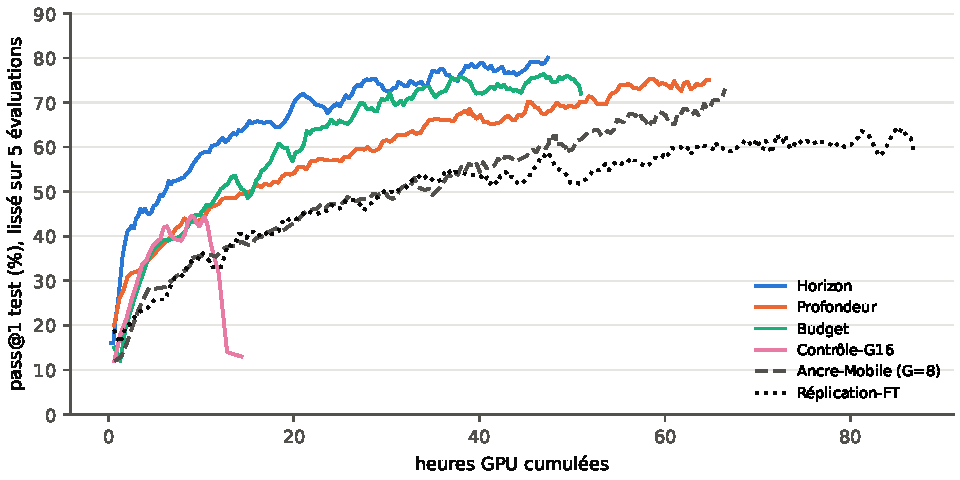
\includegraphics[width=0.9\textwidth]{figures/fig_pass1_gpuhours.pdf}
    \caption{Test pass@$1$ as a function of cumulative GPU hours. The budget curricula, \textsc{Horizon} and \textsc{Budget}, reach their plateau in 48 and 51 hours; \textsc{Depth}, which plays 30 turns from the start, needs 66; \emph{full fine-tuning} reaches 61\,\% after 86 hours.}
    \label{fig:pass1-gpuhours}
\end{figure}

\begin{figure}[htbp]
    \centering
    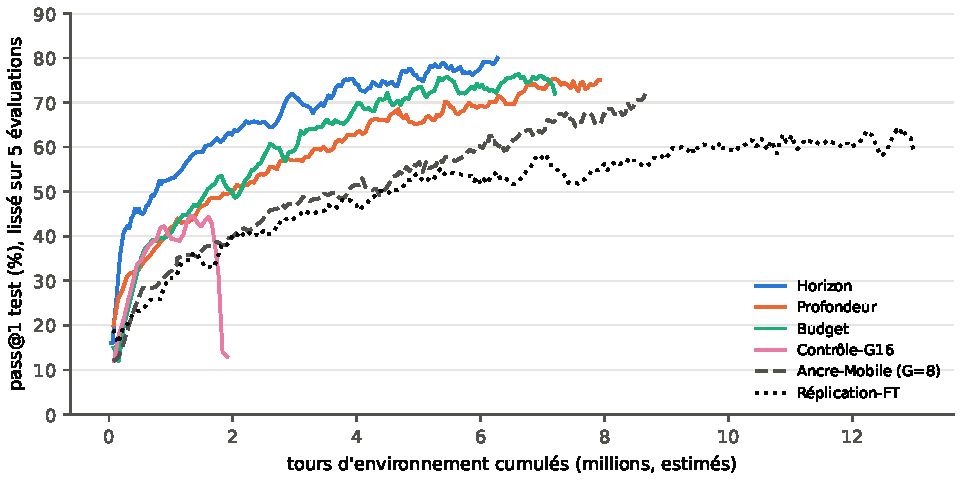
\includegraphics[width=0.9\textwidth]{figures/fig_pass1_envturns.pdf}
    \caption{Test pass@$1$ as a function of cumulative environment turns, estimated from the periodic evaluations (see text). \textsc{Horizon} reaches 78\,\% in 6.3 million turns; \emph{full fine-tuning} reaches 61\,\% in 12.4 million.}
    \label{fig:pass1-envturns}
\end{figure}

The ordering of the regimes is the same on all three axes, and the gap between curricula and references widens as the indicator moves closer to the real cost of an environment: moderate in tokens, clear in GPU hours, largest in environment turns. It is this last axis that would matter for an agent operating on a real environment, where every turn is an external call.

\subsection*{F.2 Episode Length}

\begin{figure}[htbp]
    \centering
    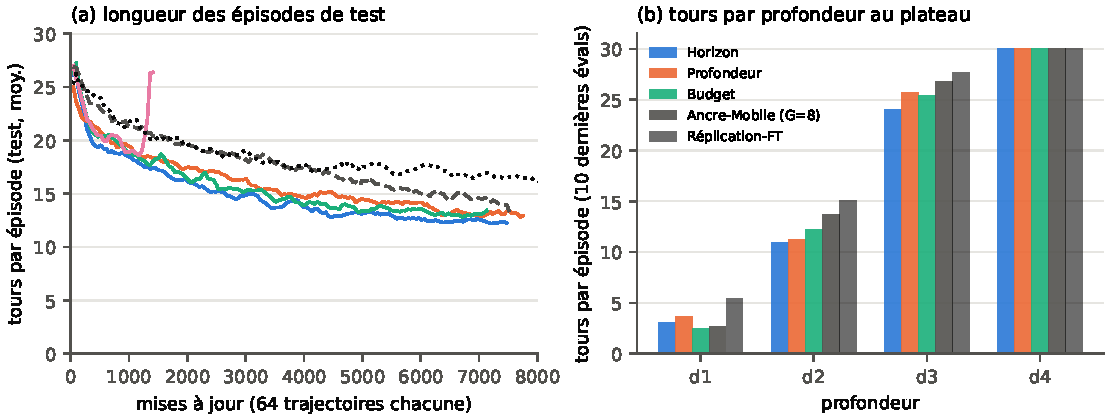
\includegraphics[width=\textwidth]{figures/explo_rounds.pdf}
    \caption{(a) Mean number of turns per test episode over the course of training. (b) Mean number of turns per depth, over the last ten evaluations of each lineage; the cap is 30 turns.}
    \label{fig:explo_rounds}
\end{figure}

The number of turns per test episode drops from 26 to 12 or 13 for the three curricula, to 14 for the reference at $G=8$ and to 16 for \emph{full fine-tuning} (Figure~\ref{fig:explo_rounds}a): the first thing reinforcement learns is efficiency, solving in fewer turns what was already being solved. The control climbs back to 26 turns at collapse, as its episodes no longer complete. The decomposition by depth (Figure~\ref{fig:explo_rounds}b) reveals a structure that pass@$1$ does not convey: at the plateau, a depth-1 task takes three turns, a depth-2 task takes eleven, a depth-3 task takes 24 to 27, and depth 4 saturates at 30. Depth-3 tasks are thus played almost up to the cap: their pass@$1$ of 30 to 45\,\% hides a majority of episodes that exhaust the thirty turns without concluding.

\subsection*{F.3 Who Produces Gradient}

\begin{figure}[htbp]
    \centering
    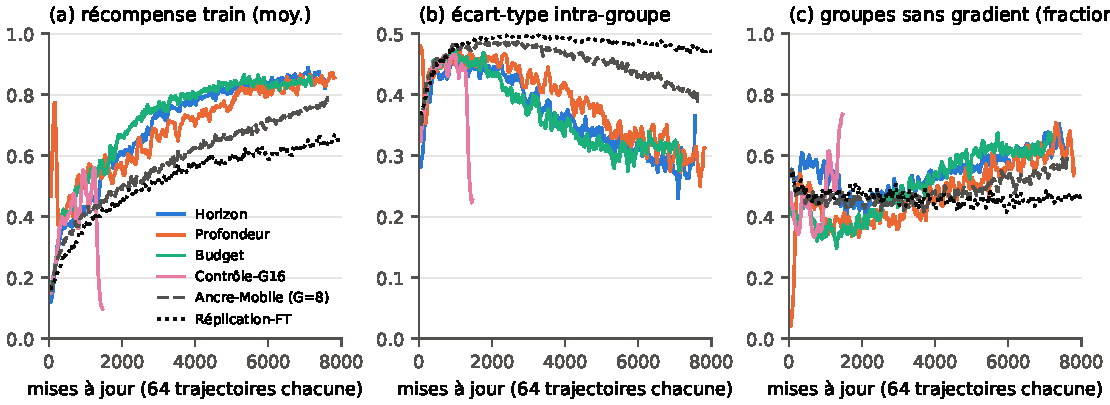
\includegraphics[width=\textwidth]{figures/explo_reward_groups.pdf}
    \caption{Per update, rolling means over one epoch. (a) Mean training reward. (b) Standard deviation of the reward within GRPO groups. (c) Fraction of groups in which all trajectories have the same reward, hence without gradient.}
    \label{fig:explo_reward_groups}
\end{figure}

Figure~\ref{fig:explo_reward_groups}c directly measures what the mechanism of Section~4.3.3 assumes: the share of GRPO groups that produce no gradient at all. From the first epochs, \textsc{Horizon} has 55 to 60\,\% of them, against 45\,\% for the control: the ten-turn cap puts the hard tasks at zero successes out of sixteen, and these groups are not punished. The control, for its part, drops toward 35\,\% uniform groups just before its collapse, which means more mixed groups with long failures, then climbs back to 75\,\% when its generations degenerate and everything fails. Over the long run, all regimes converge toward 60 to 70\,\% uniform groups, this time through saturation of the easy tasks. The intra-group standard deviation (b) tells the same story in mirror image: it decreases from 0.45 to 0.3 for the curricula as the groups become uniformly successful, and stays at 0.47 for \emph{full fine-tuning}, which remains longer in the mixed regime.

\subsection*{F.4 What the Curriculum Does to the Trajectories}

\begin{figure}[htbp]
    \centering
    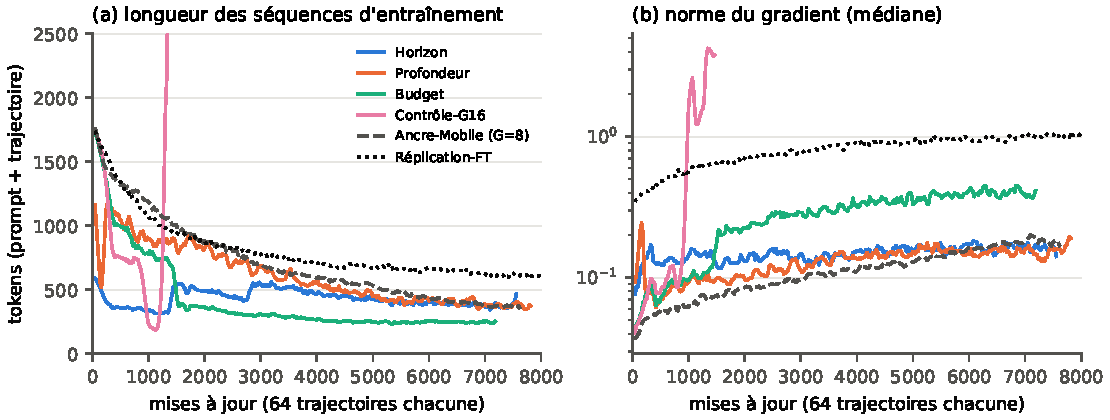
\includegraphics[width=\textwidth]{figures/explo_length_grad.pdf}
    \caption{(a) Mean length of the training sequences, prompt and trajectory included, in tokens. (b) Gradient norm, median over one epoch, logarithmic scale.}
    \label{fig:explo_length_grad}
\end{figure}

The length of the training sequences (Figure~\ref{fig:explo_length_grad}a) makes the physical action of the curricula visible. \textsc{Horizon} holds its trajectories at 350 tokens during the ten-turn stage, then jumps to 500 at epoch 15 and again at epoch 30, each time the cap is raised. \textsc{Budget} holds them at 250 tokens throughout, thanks to the generation cap. The uncapped references start from 1\,750 tokens and decrease slowly with the policy's efficiency. The control explodes beyond 2\,500 tokens at collapse. The gradient norm (b) mainly separates \emph{full fine-tuning}, around 1, from the LoRA adaptations, around 0.1; \textsc{Budget} rises to 0.4 after its budget increases, and the control diverges at collapse. We draw no conclusion from it beyond this last point.

\subsection*{F.5 The Errors, Class by Class}

\begin{figure}[htbp]
    \centering
    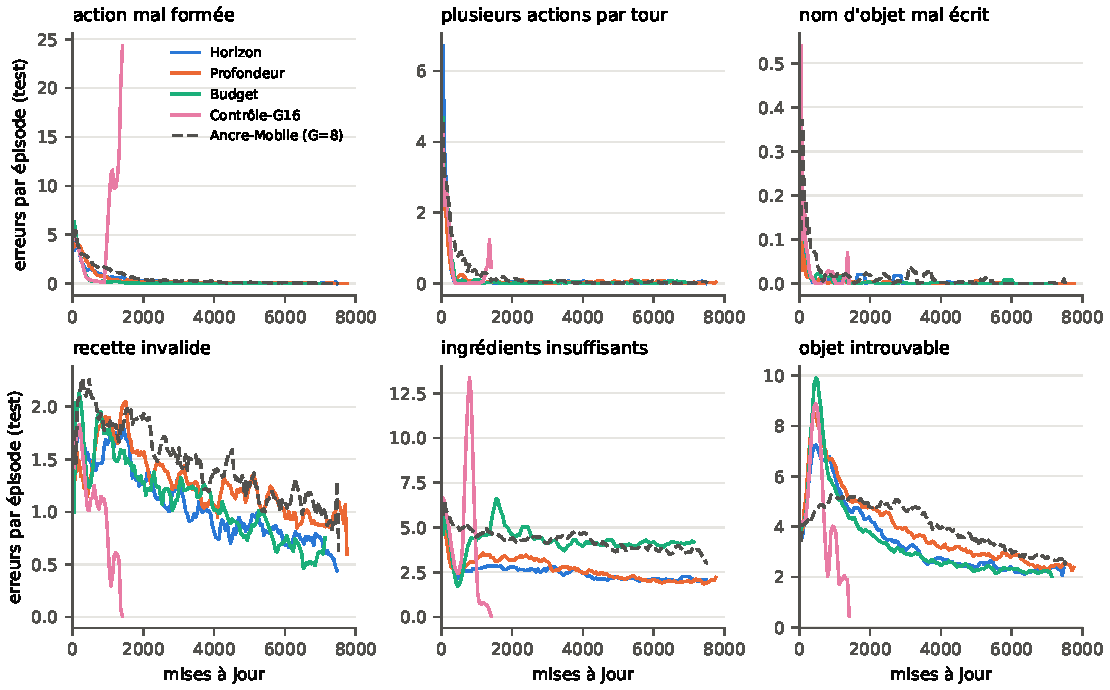
\includegraphics[width=\textwidth]{figures/fig_errors_by_type.pdf}
    \caption{Mean number of errors per test episode, for each of the six classes of the taxonomy of Section~4.1, over the course of training. Top row: format errors. Bottom row: planning errors.}
    \label{fig:errors_by_type}
\end{figure}

Figure~\ref{fig:errors_by_type} details Figure~\ref{fig:elimination_erreurs} class by class. The three format errors disappear in fewer than a thousand updates in all regimes: malformed actions, from 3 to 6 per episode at the start, and turns with several actions, from 4 to 7, fall to zero; misspelled item names were already rare. The control is the exception: its malformed actions climb back from 0 to 24 per episode at collapse, the signature of a policy that no longer produces the expected format.

The three planning errors follow different trajectories. Invalid recipes decrease slowly, from 2 to 0.5 or 1 per episode, somewhat faster with a curriculum. Items not found, that is, a \texttt{get} or a \texttt{craft} on an item absent from the inventory, first rise, from 4 to 8 or 10 per episode in the first 500 updates, before decreasing toward 2: the model first attempts more crafts with wrong names, then learns the inventory. Insufficient ingredient quantity is the most resistant class and the only one that distinguishes the regimes: \textsc{Horizon} and \textsc{Depth} bring it down from 5 or 6 to 2 per episode, the reference at $G=8$ to 3.5, but \textsc{Budget} stays at 4 throughout. One hypothesis, untested: the cap of 256 tokens per turn limits reasoning about quantities, and the model keeps launching crafts without having gathered enough ingredients. This is the only clear behavioral difference between the three curricula, whose overall scores are otherwise almost superimposed.


\subsection*{F.6 One Last Control: Group Size and Number of Tasks per Update }

Sections~4.3 and~4.4 compare the reference at $G=8$ (eight tasks of eight trajectories per update) with the control at $G=16$ (four tasks of sixteen trajectories), at 64 trajectories per update in both cases. Two things therefore change at once between these runs: the number of trajectories per task, which sets the precision of the advantage, and the number of tasks seen per update, which sets the diversity of each gradient step. The collapse of the control was attributed in the body of the report to the first factor. A run launched at the end of the internship and completed after the freeze keeps $G=16$ but moves to eight tasks per update, i.e., 128 trajectories per step and 46 steps per epoch, like the reference at $G=8$. The rest of the recipe is that of the control.

\begin{figure}[htbp]
    \centering
    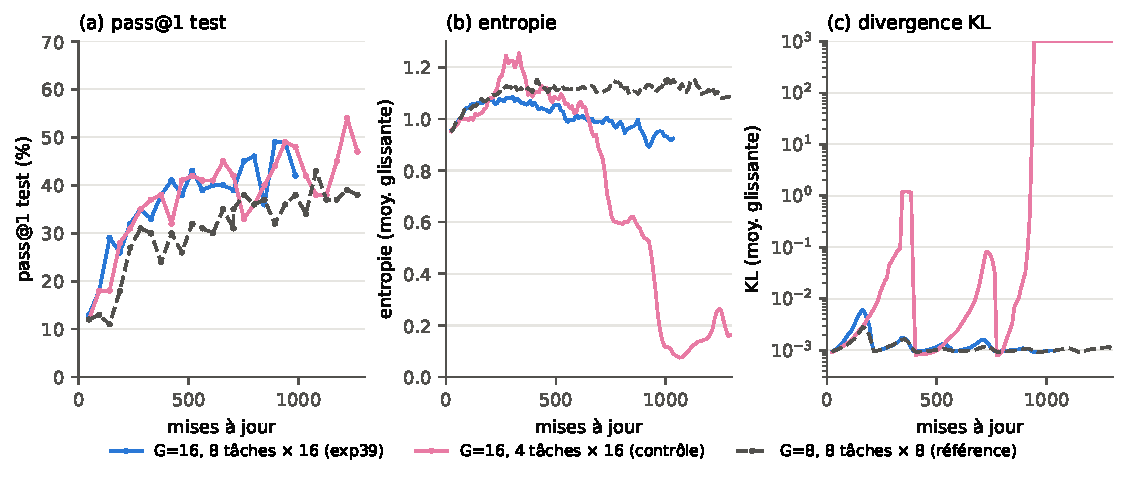
\includegraphics[width=\textwidth]{figures/fig_exp39_control.pdf}
    \caption{The run with eight tasks of sixteen trajectories (blue) compared with the control with four tasks of sixteen (pink) and the reference with eight tasks of eight (dashed), as a function of the number of updates. (a) Test pass@$1$. (b) Policy entropy. (c) KL divergence to the moving reference. At an equal number of updates, the blue run has consumed twice as many trajectories as the other two.}
    \label{fig:exp39_control}
\end{figure}

This run shows no sign of collapse over its 80 epochs; Figure~\ref{fig:exp39_control} shows the first 22. Its KL divergence stays at $10^{-3}$, brought back down at each re-anchoring. Its entropy decreases slowly, from 1.05 to 0.93 at epoch 22, like that of the reference at $G=8$. That of the control had gone from 1.0 to 0.6 and then to 0.1 over the same span. Its pass@$1$ rises steadily, from 38 to 49\,\% at epoch 22, and finishes at 72\,\%. The control was dead by the tenth epoch, the autocurriculum by the seventh. Figure~\ref{fig:exp39_vs_curricula} places it against the three curricula: at an equal number of updates, it remains some ten points below. The curriculum thus keeps its role as an accelerator.

\begin{figure}[htbp]
    \centering
    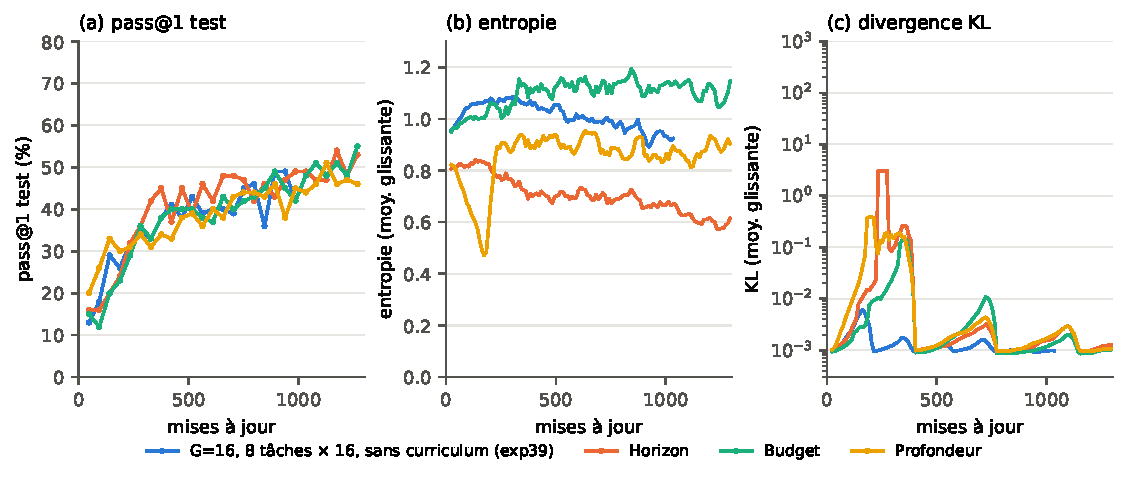
\includegraphics[width=\textwidth]{figures/fig_exp39_vs_curricula.pdf}
    \caption{The same run (blue) compared with the three curricula, as a function of the number of updates, over their first thirteen hundred updates. Same panels as the previous figure. The curricula consume half as many trajectories per update.}
    \label{fig:exp39_vs_curricula}
\end{figure}

What this run establishes is narrower than what was hoped. Against the reference at $G=8$, it changes only one thing, the group size. Its stability thus shows that $G=16$ is not sufficient, on its own, to make a run collapse. Against the control, however, it changes two things and not one. The moving anchor is defined in epochs, and this run has 46 steps per epoch against 93 for the control. Re-anchoring therefore takes place every 184 steps instead of 372. The volume of trajectories per cycle is the same, but the number of gradient steps between two resets of the KL and of the optimizer is halved. This second difference is enough to explain the stability, since Section~4.2 shows that the runs at $G=16$ reach a KL of 0.1 to 0.3 before their first re-anchoring. The collapse of the control is thus due to the move to four tasks per step, to the lengthening of the anchor cycle, or to both; this run does not separate them. The clean control was run after the freeze: the same run with re-anchoring every eight epochs, i.e., 368 steps between two anchors, like the control. It diverges through the KL at the fifteenth epoch. The collapse of the control is thus due to the lengthening of the anchor cycle in steps, not to the move to four tasks per step, and Appendix~F.7 gives its mechanism token by token. One last run completes the square: $G=8$, eight tasks per step and re-anchoring every eight epochs. It reaches 64\,\%, and stands at 60\,\% at 180\,000 trajectories against 49 for the reference re-anchored every four epochs and 50 for the run at $G=16$ with eight tasks at the same point. At equal trajectories, group size does not accelerate learning, and the re-anchoring period weighs more than $G$: each re-anchoring restarts from a fresh adapter and an empty optimizer, and this warm-up costs several epochs.



\subsection*{F.7 Token-by-Token Replay of a Collapse}

To disentangle the causes of the KL jump of the controls at $G=16$, we replayed two checkpoints of \textsc{Control-G16}, one just before the divergence, the other deep in the degenerate regime, with the training interaction loop: same prompts, same generation engine, then recomputation of the log-probabilities of the policy and of the reference on every action token by the backpropagation model. For each token, one obtains $\rho = \log \pi_{\mathrm{ref}} - \log \pi$, the estimator $k_3 = e^{\rho} - \rho - 1$, and the gap between the generation engine's log-probability and that of the recomputation.

Three facts emerge. First, the gap between engine and recomputation is not to blame: a median of $10^{-5}$ nat, some ten tokens out of a hundred thousand beyond two nats, and on those the policy and the reference agree. Second, in the degenerate regime, the entirety of the measured KL comes from the end-of-turn markers added by the interaction loop when a turn reaches its 512-token limit: two turns out of three are then truncated loops, the forced marker receives $10^{-20}$ from the policy and 0.9 from the reference, i.e., $\rho \approx 45$ and $k_3 \approx 10^{19}$ per token. Third, just before the divergence, the KL is already a hundred times that of a healthy run, and its largest terms are reasoning tokens (``Thought'') that the policy has almost stopped producing, drawn at $0.3\,\%$ where the reference expected them at $0.6$ or more ($\rho$ from 4.5 to 5.75, $k_3$ of the order of 300); turns have gone from 65 to 30 tokens and eight turns out of ten no longer contain written reasoning. The explosion observed in the logs requires $\rho \approx 18$ on a single token, a direct continuation of this trend.

The chain is therefore the following: sharpening of the policy, suppression of written reasoning, a token expected by the reference removed, an exponential and unbounded $k_3$ that dominates the update's gradient, broken format, loops until truncation, forced markers at $10^{19}$. The paper's code bounds $k_3$ to $[-10, 10]$ per token; TRL does not bound it. The \textsc{Control-G16-Bounded} run of Section~4.2.5, which adds only this bound, does not diverge (Figure~\ref{fig:bound_vs_horizon}). Figure~\ref{fig:g16_entropy_first} puts the three controls at $G=16$ back in the order of their signals: only the control re-anchored every four epochs sees its entropy decrease at length before the jump; the other two diverge first through the KL.

\begin{figure}[htbp]
    \centering
    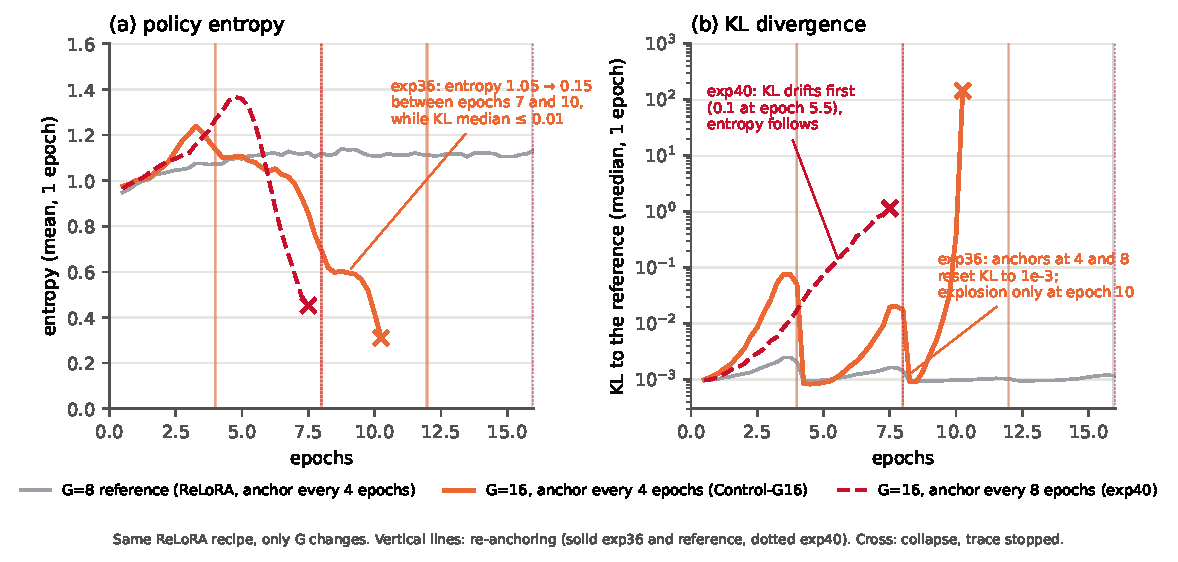
\includegraphics[width=\textwidth]{figures/fig_g16_entropy_first.pdf}
    \caption{The three no-curriculum controls at $G=16$ and the reference at $G=8$: policy entropy and KL divergence to the moving reference, per epoch. The ``entropy first'' ordering holds only for the control re-anchored every four epochs; with re-anchoring every eight or twelve epochs, the KL diverges first.}
    \label{fig:g16_entropy_first}
\end{figure}


\subsection*{F.8 A Lead: What the Curriculum Adds Once the Collapse Is Prevented}

\paragraph{What the KL penalty measures.} The exact divergence between the policy and its reference at position $t$, $\mathrm{KL}(\pi \,\|\, \pi_{\mathrm{ref}}) = \sum_{a} \pi(a \mid s_t) \log \frac{\pi(a \mid s_t)}{\pi_{\mathrm{ref}}(a \mid s_t)}$, would require summing over the whole vocabulary at every token. GRPO estimates it by Monte Carlo on the sampled tokens only: for a token $a_t$ drawn from $\pi$, one sets $\rho_t = \log \pi_{\mathrm{ref}}(a_t) - \log \pi(a_t)$ and uses the estimator $k_3 = e^{\rho} - \rho - 1$~\cite{schulman2020kl}. It is unbiased, since $\mathbb{E}_{\pi}[e^{\rho}] = \sum_a \pi_{\mathrm{ref}}(a) = 1$ and $\mathbb{E}_{\pi}[\rho] = -\mathrm{KL}$, always positive, and of much lower variance than the naive estimator $-\rho$. The KL term of the loss is the mean of $k_3$ over the action tokens, observation tokens being masked (Section~4.2.1). Its gradient with respect to $\log \pi(a_t)$ is $1 - e^{\rho_t}$: zero when policy and reference agree, it grows exponentially as soon as the policy gives a token far less probability than the reference does. The paper's code bounds $k_3$ to $[-10, 10]$ per token, which zeroes this gradient beyond $\rho \approx 2.6$, that is, as soon as the policy gives a token less than 7\,\% of the probability the reference gives it; TRL does not bound it, and Appendix~F.7 shows that a single token at $\rho = 18$ then suffices to dominate the update.

\paragraph{Motivation of the control.} Section~4.3.2 makes the curriculum a condition of stability at $G=16$, on the strength of the control's collapse. But the last link of that collapse is the unbounded estimator. An honest control therefore consists in rerunning \textsc{Control-G16} identically and changing only the bound: this is \textsc{Control-G16-Bounded}, run for 80 epochs, resumed from the saved checkpoint after an infrastructure interruption at epoch 58. If it collapses, the curriculum protects more than the bound does. If it catches up with the curricula, the curriculum's contribution must be sought elsewhere than in stability.

\paragraph{Result.} It catches up with the curricula (Figure~\ref{fig:bound_vs_horizon}). No collapse: the median KL stays at $10^{-3}$, with the sawtooth of twenty re-anchorings. Pass@$1$ reaches 82\,\% at epoch 72, like \textsc{Horizon}, for a plateau of 76 over the last ten evaluations against 78: two points, within the noise of a hundred-task evaluation. The entropy curve, however, is very different. It falls to 0.11 as early as the fourth epoch, because the bound removes the penalty's gradient on the tokens where the policy has moved furthest away, and nothing then slows the sharpening; it climbs back to 0.35 around epochs 15 to 20, then descends again to 0.13. That of \textsc{Horizon} decreases steadily from 0.8 to 0.2, with a rebound at each stage change.

\paragraph{What is left to the curriculum.} Figure~\ref{fig:bound_vs_horizon_dynamics} shows it on the trajectories themselves. During its first stage, \textsc{Horizon} plays episodes of 7 to 10 turns and about 350 tokens; at the same time, the bounded control plays 20 turns and 600 tokens. Per trajectory, the two pass@$1$ curves are superposed: the curriculum does not learn more per episode, it pays less for each episode. To reach 70\,\% as a mean of three evaluations, \textsc{Horizon} consumes 20.6 GPU hours and 2.2 million environment turns, the bounded control 29.4 hours and 3.9 million; to reach 75\,\%, 28.5 hours and 3.1 million against 39.6 hours and 5.1 million. That is 30\,\% fewer hours and 40\,\% fewer turns, for the same destination. Beyond epoch 40, the two runs have converged to the same regime, 11 to 12 turns and 350 to 400 tokens per episode, and the cost per update is equivalent. The second contribution is entropy: 0.30 on average over the second half for \textsc{Horizon}, 0.18 for the bounded control, at equal score, and turns of a dozen tokens without written reasoning for the latter. The bound avoids the symptom, the divergence; the curriculum avoids the cause, the consumption of exploration.

\paragraph{Reading.} One run per configuration, and a plateau difference within the noise: we do not conclude that the curriculum does better. We conclude that it is not the only protection against collapse at $G=16$, and that its value, once stability is secured by the bound, is twofold: a deliberate efficiency, the same level for 30\,\% less GPU and 40\,\% fewer environment turns, which matters as soon as the environment has a cost; and a guarantee of exploration, a policy twice as entropic at the same score, hence headroom to keep learning. The natural recipe combines both, bound and curriculum. One last point for future work: the $G=8$ reference without curriculum keeps 16 turns and 600 tokens per episode and an entropy close to 1 for 80 epochs, whereas all the runs at $G=16$ with four tasks per step come down to 11 turns and 0.2; it is this configuration, not the absence of a curriculum, that sharpens the policy the most.

\begin{figure}[htbp]
    \centering
    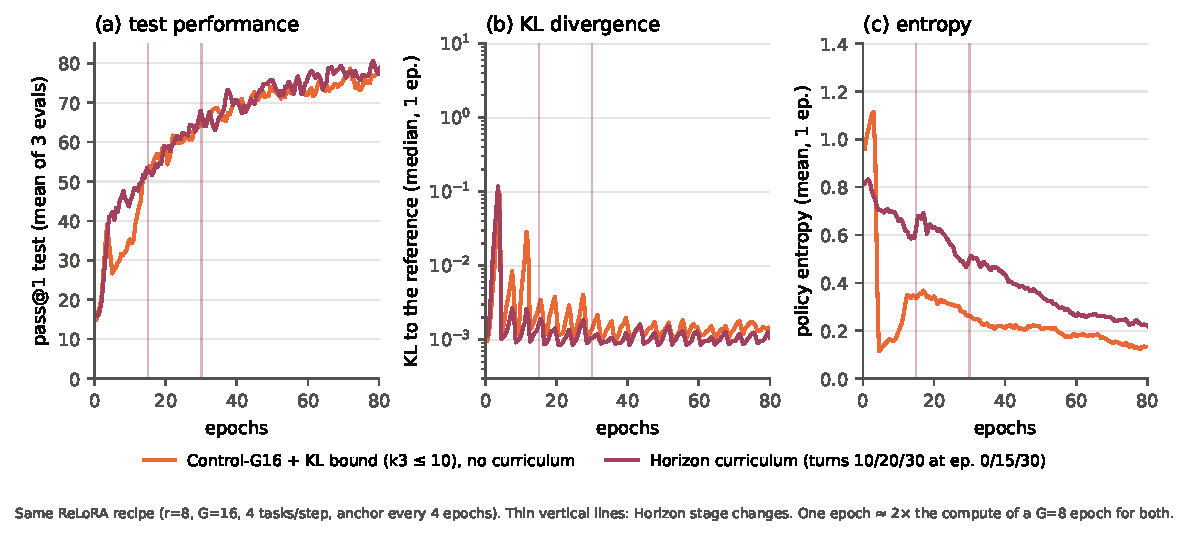
\includegraphics[width=\textwidth]{figures/fig_bound_vs_horizon.pdf}
    \caption{\textsc{Control-G16-Bounded} against \textsc{Horizon} over 80 epochs, same ReLoRA recipe ($r=8$, $G=16$, four tasks per step, anchor every 4 epochs). (a) Test pass@$1$, mean of three evaluations: same best (82), plateaus at 76 and 78. (b) KL divergence to the moving reference, median over one epoch, log scale: no divergence, sawtooth of the re-anchorings. (c) Policy entropy: collapse to 0.11 as early as the fourth epoch for the bounded control, steady descent from 0.8 to 0.2 for \textsc{Horizon}. Vertical lines: \textsc{Horizon} stage changes.}
    \label{fig:bound_vs_horizon}
\end{figure}

\begin{figure}[htbp]
    \centering
    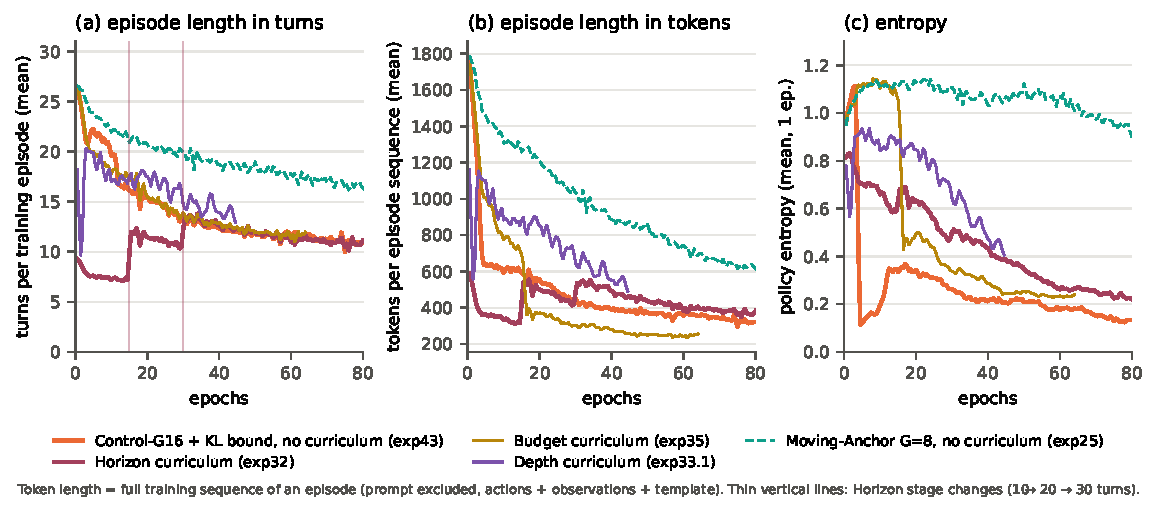
\includegraphics[width=\textwidth]{figures/fig_bound_vs_horizon_dynamics.pdf}
    \caption{Training trajectories, per epoch, of the bounded control, the three curricula and the $G=8$ reference. (a) Turns per episode: the \textsc{Horizon} cap imposes 7 to 10 turns for fifteen epochs while the bounded control plays 20; all $G=16$ runs converge to 11 to 12 turns after epoch 40, the $G=8$ reference stays at 16. (b) Tokens per episode sequence (actions, observations and template, prompt excluded). (c) Mean entropy over one epoch: the curriculum descends smoothly, the bounded control collapses and then settles twice as low.}
    \label{fig:bound_vs_horizon_dynamics}
\end{figure}

\end{document}
